\begin{ex}%[2D4C1-2]
Cho hàm số $ y=f(x)$ thỏa mãn $ f(x)<0$, $\forall x>0$ và có đạo hàm $f'(x)$ liên tục trên khoảng $\left( 0;+\infty\right) $ thỏa mãn $f'(x)=(2x+1){f^2}(x)$, $\forall x>0$ và $ f(1)=-\dfrac{1}{2}$. Tính giá trị của biểu thức $ T=f(1)+f(2)+\ldots +f\left(2023\right)+f\left(2024\right)$. (\textit{Kết quả làm tròn đến hàng đơn vị}).
\shortans{$-1$}
\loigiai{
Ta có
\begin{align*}
f'(x)=(2x+1){f^2}(x) &\Rightarrow \dfrac{f'(x)}{f^2(x)}=2x+1\\
&\Rightarrow\displaystyle\int\dfrac{f'(x)}{f^2(x)}\mathrm{\,d}x=\displaystyle\int(2x+1)\mathrm{\,d}x \\&\Rightarrow-\dfrac{1}{f(x)}=x^2+x+C.
\end{align*}
Mà $ f(1)=-\dfrac{1}{2}$ $\Rightarrow C=0$ $\Rightarrow f(x)=\dfrac{-1}{x^2+x}$ $=\dfrac{1}{x+1}-\dfrac{1}{x}$.\\
Ta có $\heva{
& f(1)=\dfrac{1}{2}-1\\
& f(2)=\dfrac{1}{3}-\dfrac{1}{2}\\
& f(3)=\dfrac{1}{4}-\dfrac{1}{3}\\
&\ldots\\
& f\left(2024\right)=\dfrac{1}{2023}-\dfrac{1}{2024}.}$\\
$
\Rightarrow T=f(1)+f(2)+\ldots+f\left(2024\right)=-1+\dfrac{1}{2025}=-\dfrac{2024}{2025}\approx -1$.}
\end{ex}

\begin{ex}%[2D4C2-2]%[Tổ 20 - Đợt 17 - Chương 4 - - CD]%[Phạm Hà Giang]
Biết $\displaystyle\int\limits_0^1 \dfrac{x^3+3x}{x^2+3x+2} \mathrm{\,d}x=a+b\ln2+c\ln3$ với $a,b,c$ là các số hữu tỉ, tính giá trị của $S=2a+b+c$.
\shortans{$-9$}
\loigiai
{ Ta có $\displaystyle\int\limits_0^1 \dfrac{x^3+3x}{x^2+3x+2} \mathrm{\,d}x=\displaystyle\int\limits_0^1 \left( x-3+\dfrac{10x+6}{x^2+3x+2}\right) \mathrm{\,d}x=\displaystyle\int\limits_0^1 \left( x-3+\dfrac{14}{x+2}-\dfrac{4}{x+1} \right) \mathrm{\,d}x=\left. \left( \dfrac{x^2}{2}-3x+14\ln \left| x+2 \right| -4\ln \left| x+1 \right| \right) \right| _0^1=-\dfrac{5}{2}+14\ln3-18\ln2$.\\
Suy ra $a=-\dfrac{5}{2}, b=-18, c=14$.\\
Vậy $S=2a+b+c=-9$.
}
\end{ex}

\begin{ex}%[Mức độ 4]%[BG12, Nguyễn Kiều Nhã Tú]%[2D4C2-2]
Cho hàm số $f(x)=\heva{&x^2+ax+b&\text{ khi }x\ge2\\&x^3-x^2-8x+10&\text{ khi }x<2 }$. Biết hàm số có đạo hàm tại điểm $x=2$. Tính $\displaystyle\int\limits_0^4 f(x)\mathrm{\,d}x$.
\SA{$4$}
\loigiai
{
Ta có $f'(x)=\heva{&2x+a&\text{ khi }x\ge2\\&3x^2-2x-8&\text{ khi }x<2.}$\\
Do hàm số có đạo hàm tại $x=2$ nên ta có
\[2\cdot2+a=0\Leftrightarrow a=-4.\]
Mặt khác, theo đề bài thì $f(x)$ liên tục tại $x=2$ hay $\lim\limits_{x\to2^+}f(x)=\lim\limits_{x\to2^-}f(x)=f(2)$.\\
Khi đó ta có phương trình
\[2^2+2a+b=-2\Leftrightarrow b=2.\]
Vậy
\begin{eqnarray*}
\displaystyle\int\limits_0^4 f(x)\mathrm{\,d}x&= & \displaystyle\int\limits_0^2 f(x)\mathrm{\,d}x+\displaystyle\int\limits_2^4 f(x)\mathrm{\,d}x\\
& = & \displaystyle\int\limits_0^2(x^3-x^2-8x+10)\mathrm{\,d}x+\displaystyle\int\limits_2^4(x^2-4x+2)\mathrm{\,d}x\\
& = & \left(\dfrac{x^4}{4}-\dfrac{x^3}{3}-4x^2+10x\right)\bigg|_0^2+\left(\dfrac{x^3}{3}-2x^2+2x\right)\bigg|_2^4\\
& = & \dfrac{16}{3}-\dfrac{4}{3}=4.
\end{eqnarray*}
}
\end{ex}

\begin{ex}%[Mức độ 4]%[BG12, Nguyễn Kiều Nhã Tú]%[2D4C2-2]
Cho hàm số $f(x)=\heva{&ax^2+bx+1,&x\ge 0\\&ax-b-1,&x<0}$. Biết rằng hàm số $f(x)$ có đạo hàm trên $\mathbb{R}$. Tính tích phân $I=\displaystyle\int\limits_{-3}^{-1} f(x)\mathrm{\,d}x$.
\SA{$10$}
\loigiai{
Hàm số có đạo hàm trên $\mathbb{R}$ nên liên tục trên $\mathbb{R}$ nên liên tục tại $x_0=0$, nghĩa là
\allowdisplaybreaks
\begin{eqnarray*}
& & f(0)=\lim\limits_{x\to 0^+}f(x)=\lim\limits_{x\to 0^-} f(x)\\
&
\Leftrightarrow & f(0)=\lim\limits_{x\to 0^+} f(x)=\lim\limits_{x\to 0^-}f(x)\\
& \Leftrightarrow & 1=\lim\limits_{x\to 0^+}(ax^2+bx+1)=\lim\limits_{x\to 0^-}(ax-b-1)\\
& \Leftrightarrow &-1-b=1\\
& \Leftrightarrow & b=-2.
\end{eqnarray*}
Suy ra $f'(x)=\heva{&2ax+b&(x\ge 0)\\&a&(x<0).}$\\
Hàm số liên tục trên $\mathbb{R}$ nên đạo hàm liên tục trên $\mathbb{R}$ nên liên tục tại $x_0=0$, nghĩa là
\allowdisplaybreaks
\begin{eqnarray*}
& & f'(0)=\lim\limits_{x\to 0^+}f'(x)=\lim\limits_{x\to 0^-}f'(x)\\
& \Leftrightarrow & b=\lim\limits_{x\to 0^+}(2ax+b)=\lim\limits_{x\to 0^-}a\\
& \Leftrightarrow & a=b=-2
\end{eqnarray*}
Từ đó suy ra $ f(x)=\heva{&-2x^2-2x+1&(x\ge 0)\\&-2x+1&(x<0).}$\\
Vậy $I=\displaystyle\int\limits_{-3}^{-1} f(x)\mathrm{\,d}x=\displaystyle\int\limits_{-3}^{-1} (-2x+1)\mathrm{\,d}x=10$.
}
\end{ex}

\begin{ex}%[Mức độ 4]%[BG12, Nguyễn Kiều Nhã Tú]%[2D4C2-2]
Cho hàm số $f(x)=\heva{&2ax,&x\le 0\\&3x^2+2bx,&x>0}$ (với $a$, $b$ là các tham số thực) thỏa $\displaystyle\int\limits_{-1}^1 f(x)\mathrm{\,d}x=2$. Giá trị nhỏ nhất của biểu thức $P=[f(-1)]^2+[f(1)]^2$ là bao nhiêu?
\SA{$12{,}5$}
\loigiai{
Ta có
\allowdisplaybreaks
\begin{eqnarray*}
& \displaystyle\int\limits_{-1}^1 f(x)\mathrm{\,d}x& =\displaystyle\int\limits_{-1}^0 f(x)\mathrm{\,d}x+\displaystyle\int\limits_0^1 f(x)\mathrm{\,d}x\\
& &=\displaystyle\int\limits_{-1}^0 2ax\mathrm{\,d}x+\displaystyle\int\limits_0^1 (3x2+2bx)\mathrm{\,d}x\\
& &=ax^2\biggl|_{-1}^0+(x^3+bx^2)\biggl|_0^1\\
& &=a+b+1
\end{eqnarray*}
Theo đề
$\displaystyle\int\limits_{-1}^1 f(x)\mathrm{\,d}x=2 \Leftrightarrow a+b+1=2\Leftrightarrow a+b=1\Leftrightarrow b=1-a$\\
Từ đó ta có
$f(x)=\heva{&2ax&(x\le 0)\\&3x^2+2(1-a)x&(x>0).}$\\
Ta có
\[P=[f(-1)]^2+[f(1)]^2=[3+2(1-a)]^2+(-2a)^2=(5+2a)^2+4a^2=25+20a+4a^2+4a^2=8a^2+20a+25.\]
Xét $P'=16a+20$, $P'=0\Leftrightarrow a=-\dfrac{5}{4}$.\\
Bảng biến thiên\\
\begin{center}

\begin{tikzpicture}[>=stealth]
\tkzTabInit[nocadre=false,lgt=1,espcl=2,deltacl=0.5]{$x$/.7 ,$y'$/.7,$y$/2}
{$-\infty$ , $-\dfrac{5}{4}$ , $+\infty$}
\tkzTabLine{ , - , $0$ , + , }
\tkzTabVar{+/$+\infty$ , -/$\dfrac{25}{2}$ , +/$+\infty$}
\end{tikzpicture}
\end{center}
Vậy $\min P=\dfrac{25}{2}$ khi $a=\dfrac{-5}{4}$.
}
\end{ex}

\begin{ex}%[2D4C2-3]%[Tổ 20 - Đợt 17 - Chương 4 - - CD]%[Nguyễn Hồng Thạch]
Một vật chuyển động với gia tốc được cho bởi hàm số $a(t)=5\cos\left(t+\dfrac{\pi}{6}\right)$ (m/$\mathrm{s}^2$). Lúc bắt đầu chuyển động vật có vận tốc $2$ m/$\mathrm{s}^2$. Tính quãng đường vật di chuyển từ khi xuất phát đến thời điểm vật có vận tốc đạt giá trị lớn nhất ở lần đầu tiên.
\shortans{$3{,}8$}
\loigiai
{Vận tốc của vật được biểu diễn bởi hàm số \[v(t)=\displaystyle\int a(t)\mathrm{\,d}t=\displaystyle\int 5\cos\left(t+\dfrac{\pi}{6}\right)\mathrm{\,d}t=5\sin\left(t+\dfrac{\pi}{6}\right)+C\]
Khi bắt đầu chuyên động (tức là $t=0$), vật có vận tốc $2$ m/$\mathrm{s}^2$ nên ta có\[v\left(0+\dfrac{\pi}{6}\right)=2\Leftrightarrow 5\sin\dfrac{\pi}{6}+C=2\Rightarrow C=-\dfrac{1}{2}\]
Suy ra $v(t)=5\sin\left(t+\dfrac{\pi}{6}\right)-\dfrac{1}{2}$.\\
Mà $5\sin\left(t+\dfrac{\pi}{6}\right)-\dfrac{1}{2}\leq \dfrac{9}{2}$.\\
Suy ra vận tốc đạt giá trị lớn nhất ở lần đầu tiên khi và chỉ khi \[\sin\left(t+\dfrac{\pi}{6}\right)=1\Leftrightarrow t+\dfrac{\pi}{6}=\dfrac{\pi}{2}\Leftrightarrow t=\dfrac{\pi}{3}\]
Vậy quãng đường vật đi được từ khi xuất phát đên thời điểm $t=\dfrac{\pi}{3}$ là
\[s=\displaystyle\int\limits_{0}^{\frac{\pi}{3}}\left(5\sin\left(t+\dfrac{\pi}{6}\right)-\dfrac{1}{2}\right)\mathrm{\,d}t=\left(-5\cos\left(t+\dfrac{\pi}{6}\right)-\dfrac{t}{2}\right)\Big|_0^{\frac{\pi}{3}}=\dfrac{5\sqrt{3}}{2}-\dfrac{\pi}{6}\approx 3{,}8~\mathrm{m}\]
}
\end{ex}

\begin{ex}%[2D4C2-3]
Cho hàm số $y=f(x)$ xác định trên $\left[0;\dfrac{\pi}{2}\right]$ thoả mãn $\break \displaystyle \int\limits_0^{\tfrac{\pi}{2}} \left[f^2(x)-2\sqrt{2}f(x)\sin\left(x-\dfrac{\pi}{4}\right)\right]\mathrm{\,d}x=\dfrac{2-\pi}{2}$. Tích phân $\displaystyle \int\limits_0^{\tfrac{\pi}{2}} f(x)\mathrm{\,d}x$ bằng
\shortans[]{$0$}
\loigiai{
Ta có \[ \displaystyle \int\limits_0^{\tfrac{\pi}{2}} 2\sin^2\left(x-\dfrac{\pi}{4}\right)\mathrm{\,d}x=\displaystyle \int\limits_0^{\tfrac{\pi}{2}} \left(1-\sin 2x\right)\mathrm{\,d}x=\left(x+\dfrac{\cos 2x}{2}\right)\Big|_0^{\tfrac{\pi}{2}}=\dfrac{\pi-2}{2}. \]
Dẫn tới
\begin{eqnarray*}
& & \displaystyle \int\limits_0^{\tfrac{\pi}{2}} \left[f^2(x)-2\sqrt{2}f(x)\sin\left(x-\dfrac{\pi}{4}\right)+2\sin^2\left(x-\dfrac{\pi}{4}\right)\right]\mathrm{\,d}x=0 \\
&\Leftrightarrow& \displaystyle \int\limits_0^{\tfrac{\pi}{2}} \left[f(x)-\sqrt{2}\sin\left(x-\dfrac{\pi}{4}\right)\right]^2\mathrm{\,d}x=0 \\
&\Leftrightarrow& \displaystyle \int\limits_0^{\tfrac{\pi}{2}} \left[f(x)-\sqrt{2}\sin\left(x-\dfrac{\pi}{4}\right)\right]\mathrm{\,d}x=0.
\end{eqnarray*}
Hay ta có \[ \displaystyle \int\limits_0^{\tfrac{\pi}{2}} f(x)\mathrm{\,d}x=\int\limits_0^{\tfrac{\pi}{2}} \sqrt{2}\sin\left(x-\dfrac{\pi}{4}\right)\mathrm{\,d}x=-\sqrt{2}\cos\left(x-\dfrac{\pi}{4}\right)\Big|_0^{\tfrac{\pi}{2}}=0. \vspace{-2em} \]
}
\end{ex}

\begin{ex}%[Mức độ 4]%[Dat Thai, Dự án giảng 12 New]%[2D4C2-3]
Cho tích phân $I=\displaystyle\int\limits_{\tfrac{\pi }{2}}^{\pi }\dfrac{(12\cos x-5\sin x+10)\mathrm{\,d}x}{2\sin x+3\cos x+5}=a\pi +b\ln 2-c\ln 7$; với $a, b, c$ là những số nguyên dương. Tính giá trị của biểu thức $T=a+b+c$.
\shortans{$7$}
\loigiai{
\begin{itemize}
\item Đây là dạng tích phân khó, ta tiến hành phân tích tử số theo mẫu số
\[
TS=f(x)\cdot MS +\beta\cdot MS',
\]
trong đó $f(x)$ có thể là hằng số có thể là một hàm số đơn giản và $\beta$ chắc chắn là hằng số.
\item Ta có $12\cos x-5\sin x+10\equiv f(x)\cdot (2\sin x+3\cos x+5)+\beta(2\cos x-3\sin x)$.
\item $12\cos x-5\sin x+10\equiv (2f(x)-3\beta)\sin x+(3f(x)+2\beta)\cos x+5\cdot f(x)\\
\Leftrightarrow $$\heva{&2f(x)-3\beta=-5 \\& 3f(x)+2\beta=12 \\& 5\cdot f(x)=10} \Leftrightarrow \heva{&f(x)=2 \\& \beta=3.}$
\item Khi đó
\begin{eqnarray*}
I=\displaystyle\int\limits_{\tfrac{\pi }{2}}^{\pi }\dfrac{(12\cos x-5\sin x+10)\mathrm{\,d}x}{2\sin x+3\cos x+5}&=&\displaystyle\int\limits_{\tfrac{\pi }{2}}^{\pi }\left(2+3\cdot \dfrac{2\cos x-3\sin x}{2\sin x+3\cos x+5}\right)\mathrm{\,d}x\\
&=&(2x+3\ln |2\sin x+3\cos x+5|)\bigg|_{\tfrac{\pi }{2}}^{\pi }\\
&=&\pi +3\ln 2-3\ln 7.
\end{eqnarray*}
Suy ra $a=1$; $b=3$; $c=3$ hay $T=a+b+c=7$.
\end{itemize}
}
\end{ex}

\begin{ex}%[2D4C2-4]
Cho hàm số $f(x)$ liên tục trên $\mathbb{R}$ và thỏa mãn $\displaystyle\int\limits_0^{\tfrac{\pi}{4}} \tan x\cdot f(\cos^2 x)\mathrm{\,d}x=2$; $\displaystyle\int\limits_{\mathrm{e}}^{\mathrm{e}^2} \dfrac{f(\ln^2 x)}{x\ln x}\mathrm{\,d}x=2$. Khi đó $\displaystyle\int\limits_{\tfrac{1}{4}}^2 \dfrac{f(2x)}{x}\mathrm{\,d}x$ có giá trị bằng bao nhiêu?
\shortans{$8$}

\loigiai{
\begin{itemize}
\item Ta có $I_1=\displaystyle\int\limits_0^{\tfrac{\pi}{4}} \tan x\cdot f(\cos^2 x)\mathrm{\,d}x=\dfrac{1}{2}\displaystyle\int\limits_0^{\tfrac{\pi}{4}} \dfrac{f(\cos^2 x)}{\cos^2 x}\cdot\sin 2x\mathrm{\,d}x$.\\
Đặt $t=\cos^2 x \Rightarrow \sin 2x\mathrm{\,d}x=-\mathrm{\,d}t$.\\
Khi đó $I_1=-\dfrac{1}{2}\displaystyle\int\limits_1^{\tfrac{1}{2}} \dfrac{f(t)}{t}\mathrm{\,d}x\Rightarrow \displaystyle\int\limits_{\tfrac{1}{2}}^1 \dfrac{f(t)}{t}\mathrm{\,d}x=4$.
\item Lại có $I_2=\displaystyle\int\limits_{\mathrm{e}}^{\mathrm{e}^2} \dfrac{f(\ln^2 x)}{x\ln x}\mathrm{\,d}x=\dfrac{1}{2}\displaystyle\int\limits_{\mathrm{e}}^{\mathrm{e}^2} \dfrac{f(\ln^2 x)}{\ln^2 x}\cdot\dfrac{2\ln x}{x}\mathrm{\,d}x$.\\
Đặt $t=\ln^2 x \Rightarrow \dfrac{2\ln x}{x}\mathrm{\,d}x=\mathrm{\,d}t$.\\
Khi đó $I_2=\dfrac{1}{2}\displaystyle\int\limits_1^4 \dfrac{f(t)}{t}\cdot\mathrm{\,d}x\Rightarrow \displaystyle\int\limits_1^4 \dfrac{f(t)}{t}\cdot\mathrm{\,d}x=4$.
\item Tính $I=\displaystyle\int\limits_{\tfrac{1}{4}}^{2} \dfrac{f(2x)}{x}\mathrm{\,d}x$. \\
Đặt $t=2x \Rightarrow \mathrm{\,d}x=\dfrac{1}{2}\mathrm{\,d}t$.\\
Vậy $I=\displaystyle\int\limits_{\tfrac{1}{2}}^4 \dfrac{f(t)}{t}\mathrm{\,d}t=\displaystyle\int\limits_{\tfrac{1}{2}}^{1} \dfrac{f(t)}{t}\mathrm{\,d}t+\displaystyle\int\limits_1^4 \dfrac{f(t)}{t}\mathrm{\,d}t=4+4=8$.
\end{itemize}
}
\end{ex}

\begin{ex}%[Mức độ 4]%[Dat Thai, Dự án giảng 12 New]%[2D4C2-4]
Cho tích phân $I=\displaystyle\int\limits_0^{\ln 2}\dfrac{x\mathrm{\,d}x}{x+\mathrm{e}^{-x}}=a\ln 2+b\ln \left(\ln 2+\dfrac{1}{2}\right)$, với $a, b$, là những số nguyên dương. Tính giá trị của biểu thức $T=a^2+b^2+3ab$.
\shortans{$5$}
\loigiai{
Ta có
\begin{eqnarray*}
I=\displaystyle\int\limits_0^{\ln 2}\dfrac{(x+1)\mathrm{\,d}x}{x+\mathrm{e}^{-x}}&=&\displaystyle\int\limits_0^{\ln 2}\dfrac{\left(x+\mathrm{e}^{-x}-\mathrm{e}^{-x}+1\right)\mathrm{\,d}x}{x+\mathrm{e}^{-x}}\\&=&\displaystyle\int\limits_0^{\ln 2}\dfrac{\left(x+\mathrm{e}^{-x}\right)\mathrm{\,d}x}{x+\mathrm{e}^{-x}}+\displaystyle\int\limits_0^{\ln 2}\dfrac{\left(1-\mathrm{e}^{-x}\right)\mathrm{\,d}x}{x+\mathrm{e}^{-x}}\\&=&\displaystyle\int\limits_0^{\ln 2}\mathrm{\,d}x+\ln \left|x+\mathrm{e}^{-x}\right|\bigg|_0^{\ln 2}.
\end{eqnarray*}
Do đó $I=\displaystyle\int\limits_0^{\ln 2}\mathrm{\,d}x+\ln \left|x+\mathrm{e}^{-x}\right|\bigg|_0^{\ln 2}=\ln 2+\ln \left(\ln 2+\dfrac{1}{2}\right)=a\ln 2+b\ln \left(\ln 2+\dfrac{1}{2}\right)$.\\
Vậy $a=1$; $b=1$ hay $T=a^2+b^2+3ab=5$.
}
\end{ex}

\begin{ex}%[Dự án phát triển đề ĐGNL 2025]%[Nguyễn Thành Nhân]%[2D4C2-4]
Cho hàm số $f(x)$ có đạo hàm liên tục trên $\mathbb{R}$, $f(0)=0$, $f'(0)\neq 0$ và thỏa mãn hệ thức $f(x)f'(x)+18x^2=(3x^2+x)f'(x)+(6x+1)f(x)$, $\forall x\in \mathbb{R}$. Biết $\displaystyle\int\limits_0^1 (x+1)\mathrm{e}^{f(x)}\mathrm{\,d}x=a\mathrm{e}^2+b$, với $a, b\in \mathbb{Q}$. Giá trị của $a-b$ bằng
\shortans{$1$}
\loigiai{
Ta có $f(x)f'(x)+18x^2=(3x^2+x)f'(x)+(6x+1)f(x)$\\
$\Rightarrow \left[\dfrac{1}{2}f^2(x)+6x^3\right]'=\left[(3x^2+x)f(x)\right]'$\\
$\Rightarrow \dfrac{1}{2}f^2(x)+6x^3=(3x^2+x)f(x)+C$, với $C$ là hằng số.\\
Mặt khác, theo giả thiết $f(0)=0$ nên $C=0$.\\
Khi đó $\dfrac{1}{2}f^2(x)+6x^3=(3x^2+x)f(x)$, $\forall x\in \mathbb{R}$. Ta có
\begin{eqnarray*}
&& \dfrac{1}{2}f^2(x)+6x^3=(3x^2+x)f(x)\\
&\Leftrightarrow & f^2(x)+12x^3=(6x^2+2x)f(x)\\
&\Leftrightarrow & \left[f(x)-2x\right]\left[f(x)-6x^2\right]=0\\
&\Leftrightarrow & \hoac{& f(x)=2x \\ & f(x)=6x^2.}
\end{eqnarray*}
\begin{itemize}
\item Với $f(x)=6x^2$, $\forall x\in \mathbb{R}$, ta có $f'(0)=0$ (loại).
\item Với $f(x)=2x$, $\forall x\in \mathbb{R}$, ta có
\begin{eqnarray*}
\displaystyle\int\limits_0^1 (x+1)\mathrm{e}^{f(x)}\mathrm{\,d}x&=&\int\limits_0^1(x+1)\mathrm{e}^{2x}\mathrm{\,d}x\\
&=&\left. \left[\dfrac{(x+1)\mathrm{e}^{2x}}{2}\right]\right|_0^1-\dfrac{1}{2}\int\limits_0^1\mathrm{e}^{2x}\mathrm{\,d}x\\
&=&\dfrac{3}{4}\mathrm{e}^2-\dfrac{1}{4}\\
&\Rightarrow & \heva{& a=\dfrac{3}{4} \\ & b=-\dfrac{1}{4}}\Rightarrow a-b=1
\end{eqnarray*}
\end{itemize}
}
\end{ex}

\begin{ex}%[2D4C2-6]
Một vật chuyển động với vận tốc tăng liên tục được biểu thị bằng đồ thị là đường cong parabol ở hình bên dưới.
\begin{center}
\begin{tikzpicture}[>=stealth]
\draw[->] (-0.5,0) --(0,0) node[below
right]{$O$} -- (5,0)
node[below]{$t(s)$};
\draw[->](0,-0.5)--(0,5)
node[right]{$v(m)$};
\draw[smooth,blue,line width=1]
plot[domain=0:4]
(\x,{-(\x)^(2)+4*\x});
\draw[dashed] (0,4) node[left]{} -- (2,4) --(2,0);
\draw (2,0) node[below] {$10$};
\draw (0,4) node[left] {$50$};
\end{tikzpicture}
\end{center}
Biết rằng sau $10$s thì vật đó đạt đến vận tốc cao nhất và bắt đầu giảm tốc. Hỏi từ lúc bắt đầu đến lúc đạt vận tốc cao nhất thì vật đó đi được quãng đường bao nhiêu mét (làm tròn đến chữ số hàng đơn vị)?
\shortans{333}
\loigiai{Giả sử vận tốc của vật biểu diển bởi hàm số $(P)\colon v(t)=a t^2+b t+c \quad(a \neq 0)$.\\
Dựa vào đồ thị hàm số ta có $(P)$ đi qua $O(0 ; 0)$ và có đỉnh $I(10 ; 50)$.
\[
\Rightarrow \heva{&
c = 0  \\ &
1 0 0 a + 1 0 b = 5 0 \\&
- \dfrac { b } { 2 a } = 1 0 }
\Rightarrow
\heva {&
c = 0  \\&
1 0 a + b = 5 \\&
2 0 a + b = 0 }
\Rightarrow
\heva {&
c=0 \\&
a=-\dfrac{1}{2} \\&
b=10}
\Rightarrow (P) \colon v(t)=-\dfrac{1}{2} t^2+10 t.\]
Lúc bắt đầu: $t=0$ s; lúc đạt vận tốc cao nhất: $t=10$ s.\\
Vậy quãng đường vận đó đi được kể từ lúc bắt đầu đến lúc đạt vận tốc cao nhất là
\[s=\displaystyle\int\limits_0^{10} v(t) \mathrm{\,d} t=\displaystyle\int\limits_0^{10}\left(-\dfrac{1}{2} t^2+10 t\right) \mathrm{\,d} t=\dfrac{1000}{3}\simeq 333.\]
}
\end{ex}

\begin{ex}%[2D4C2-6]Biên soạn:Phùng Hoàng Em Phản biện:Nguyễn Đắc Kiên
Tại một nhà máy sản xuất một loại phân bón, gọi $P(x)$ là lợi nhuận (tính theo triệu đồng) thu được từ việc bán $x$ tấn sản phẩm trong một tuần. Khi đó, đạo hàm $P^{\prime}(x)$, gọi là lợi nhuận cận biên, cho biết tốc độ tăng lợi nhuận theo lượng sản phẩm bán được. Giả sử lợi nhuận cận biên (tính theo triệu đồng trên tấn) của nhà máy được ước lượng bởi công thức
\[
P^{\prime}(x)=16-0{,}02 x \text { với } 0 \leq x \leq 100.
\]
Tính lợi nhuận (triệu đồng) nhà máy thu được khi bán $90$ tấn sản phẩm trong tuần. Biết rằng nhà máy lỗ $25$ triệu đồng nếu không bán được lượng sản phẩm nào trong tuần.
\shortans{$1334$}
\loigiai{
Ta có $P(0)=-25$ (lỗ khi không bán được lượng sản phẩm nào trong tuần)
\[
\begin{aligned}
P(90)-P(0) &=\displaystyle\int\limits_0^{90} P^{\prime}(x) \mathrm{\,d}x=\displaystyle\int\limits_0^{90}(16-0{,}02 x) \mathrm{\,d} x \\
&=16 \displaystyle\int\limits_0^{90} \mathrm{\,d} x-0{,}02 \displaystyle\int\limits_0^{90} x \mathrm{\,d} x \\
&=\left.16 x\right|_0 ^{90}-0{,}01 x^2\left.\right|_0 ^{90}=1359.
\end{aligned}
\]
Suy ra $P(90)=P(0)+1359=-25+1359=1334$ (triệu đồng).\\
Vậy lợi nhuận nhà máy thu được khi bán $90$ tấn sản phẩm trong tuần là $1334$ triệu đồng.
}
\end{ex}

\begin{ex}%[2D4C2-6]
\immini[thm]{Cho hàm số $ y=x^4-mx^2$ có đồ thị $\left(C_m\right)$ với $m>0$. Hình phẳng tạo bởi $\left(C_m\right)$ và trục $Ox$ gồm hai phần có diện tích $S_1$ và $S_2$ như hình vẽ. Tìm $m$ để $S_1+S_2=\dfrac{16\sqrt{2}}{15}$.
}
{
\begin{tikzpicture}[scale=1,>=stealth, font=\footnotesize, line join=round, line cap=round]
\def\a{1} \def\b{-2} \def\c{0} % Hệ số
\def\xmin{-2} \def\xmax{2.5}
\def\ymin{-1.5} \def\ymax{2}
%	\draw[color=gray!50,dashed] (\xmin,\ymin) grid (\xmax,\ymax);
\draw[->] (\xmin,0)--(\xmax,0) node [below]{$x$};
\draw[->] (0,\ymin)--(0,\ymax) node [left]{$y$};
\node at (0,0) [above left]{$O$};
\clip (\xmin+0.1,\ymin+0.1) rectangle (\xmax-0.5,\ymax-0.1);
\draw[smooth,samples=300] plot(\x,{\a*(\x)^4+\b*(\x)^2+\c});
\fill[pattern=north east lines,opacity=0.8] plot[domain=-sqrt(2):sqrt(2)](\x,{\a*(\x)^4+\b*(\x)^2+\c})--cycle;
\draw(-0.7,0)node[below,scale=0.9]{$S_1$}
(0.7,0)node[below,scale=0.9]{$S_2$}
;
\end{tikzpicture}
}
\shortans{2}
\loigiai{
\immini{Ta có $x^4-mx^2=0\Leftrightarrow x^2\left(x^2-m\right)=0\Leftrightarrow\hoac{
& x=0\\
& x=\sqrt{m}\\
& x=-\sqrt{m}}$ vì $m>0$.\\
Do hàm số $ y=x^4-mx^2$ là hàm chẵn nên đồ thị hàm số đối xứng qua trục $Oy$ $\Rightarrow{S_1}=S_2\Rightarrow{S_1}+S_2=2S_2$.
}
{
\begin{tikzpicture}[scale=1,>=stealth, font=\footnotesize, line join=round, line cap=round]
\pgfmathsetmacro{\aa}{sqrt(2)}
%\def\aa{sqrt2}
\def\a{1} \def\b{-2} \def\c{0} % Hệ số
\def\xmin{-2.5} \def\xmax{3}
\def\ymin{-1.5} \def\ymax{2}
%	\draw[color=gray!50,dashed] (\xmin,\ymin) grid (\xmax,\ymax);
\draw[->] (\xmin,0)--(\xmax,0) node [below]{$x$};
\draw[->] (0,\ymin)--(0,\ymax) node [left]{$y$};
\node at (0,0) [above left]{$O$};
\clip (\xmin+0.1,\ymin+0.1) rectangle (\xmax-0.5,\ymax-0.1);
\draw[smooth,samples=300] plot(\x,{\a*(\x)^4+\b*(\x)^2+\c});
\fill[pattern=north east lines,opacity=0.8] plot[domain=-sqrt(2):sqrt(2)](\x,{\a*(\x)^4+\b*(\x)^2+\c})--cycle;
\draw(-0.7,0)node[below,scale=0.9]{$S_1$}
(0.7,0)node[below,scale=0.9]{$S_2$}
;
\draw[fill=black](-\aa,0)node[below left,scale=0.8]{$-\sqrt m$}circle(1pt)
(\aa,0)node[below right]{$\sqrt m$}circle(1pt)
;
\end{tikzpicture}
}
\noindent
Mà $S_2=\displaystyle\int\limits_0^{\sqrt{m}}\left(m{x^2}-x^4\right)\mathrm{d}x=\left(\dfrac{mx^3}{3}-\dfrac{x^5}{5}\right)\bigg|_0^{\sqrt{m}}=\dfrac{2m^2\sqrt{m}}{15}$.\\
Vì $S_1+S_2=\dfrac{16\sqrt{2}}{15}\Leftrightarrow 2S_2=\dfrac{16\sqrt{2}}{15}\Leftrightarrow\dfrac{4m^2\sqrt{m}}{15}=\dfrac{16\sqrt{2}}{15}\Leftrightarrow m^2\sqrt{m}=4\sqrt{2}\Leftrightarrow m=2$.\\
Vậy $m=2$.}
\end{ex}

\begin{ex}%[2D4C3-1]
Xét hàm số $f(x)=ax^3+bx^2+cx+d$ $\left( a,b,c,d \in \mathbb{R};a>0 \right)$ có hai cực trị $x_1$, $x_2$ (với $x_1<x_2$) thỏa mãn $x_1+x_2=0$. Hình phẳng giới hạn bởi đường $y=f'(x)f'' (x)$ và trục hoành có diện tích bằng $\dfrac{9}{4}$. Biết $\displaystyle \int\limits_{x_1}^{x_2} \dfrac{f'(x)}{3^x+1}\mathrm{\,d}x=-\dfrac{7}{2}$, giá trị của $\displaystyle \int\limits_0^{x_2} (x+2)f'' (x)\mathrm{\,d}x$ bằng bao nhiêu? (làm tròn kết quả đến hàng phần chục)
\shortans[0]{6,5}
\loigiai{
Ta có $f(x)=ax^3+bx^2+cx+d
\Rightarrow f'(x)=3ax^2+2bx+c$.\\
Do $f(x)$ có hai cực trị $x_1,x_2$ (với $x_1<x_2$) nên $f'(x)=0$ có hai nghiệm $x_1$, $x_2$.\\
Vì $x_1+x_2=0$ nên $\dfrac{-2b}{3a}=0\Rightarrow b=0$ suy ra $f'(x)=3ax^2+c\Rightarrow f'' (x)=6ax$.\\
Ta có $f'(x)f'' (x)=0\Leftrightarrow \hoac{&x=x_1\\&x=0\\&x=x_2.}$
\begin{center}

\begin{tikzpicture}
\tkzTabInit[nocadre=false,lgt=4,espcl=2,deltacl=0.6]
{$x$ /0.6,$f'(x)$ /0.6,$f'' (x)$/0.6,$y=f'(x)\cdot f'' (x)$/0.6}
{$-\infty$,$x_1$,$0$,$x_2$,$+\infty$}
\tkzTabLine{,+,$0$,-,z,-,$0$,+,}
\tkzTabLine{,-,z,-,$0$,+,$0$,+,}
\tkzTabLine{,-,$0$,+,$0$,-,$0$,-,}
\end{tikzpicture}
\end{center}
Hình phẳng giới hạn bởi đường $y=f'(x)f'' (x)$ và trục hoành có diện tích bằng $\dfrac{9}{4}$.\\
Suy ra \[\dfrac{9}{4}=\displaystyle \int\limits_{x_1}^{x_2} \left| f'(x)f'' (x) \right|\mathrm{\,d}x
=\displaystyle \int\limits_{x_1}^0 f'(x)f'' (x)\mathrm{\,d}x-\displaystyle \int\limits_0^{x_2} f'(x)f'' (x)\mathrm{\,d}x
=\left. \dfrac{1}{2}{{\left[ f'(x) \right]}^2} \right|_{x_1}^0-\left. \dfrac{1}{2}{{\left[ f'(x) \right]}^2} \right|_0^{x_2}=c^2\] $\Rightarrow c=-\dfrac{3}{2}$ (do $c<0$)\\
Suy ra $f'(x)=3ax^2-\dfrac{3}{2}
\Rightarrow \hoac{& {x_1}=-\sqrt{\dfrac{1}{2a}} \\& {x_2}=\sqrt{\dfrac{1}{2a}}.}$\\
Ta có $\displaystyle \int\limits_{x_1}^{x_2} \dfrac{f'(x)}{3^x+1}\mathrm{\,d}x
=\displaystyle \int\limits_{x_1}^0 \dfrac{f'(x)}{3^x+1}\mathrm{\,d}x + \displaystyle \int\limits_0^{x_2} \dfrac{f'(x)}{3^x+1}\mathrm{\,d}x$\\
Xét $A=\displaystyle \int\limits_{x_1}^0 \dfrac{f'(x)}{3^x+1}\mathrm{\,d}x$. Đặt $t=-x$.\\
Ta có $A=-\displaystyle \int\limits_{-x_1}^0 \dfrac{f'\left( -t \right)}{{3^{-t}}+1}\mathrm{\,d}t
=\displaystyle \int\limits_0^{-x_1} \dfrac{3^tf'(t)}{3^t+1}\mathrm{\,d}t
=\displaystyle \int\limits_0^{x_2} \dfrac{3^xf'(x)}{3^x+1}\mathrm{\,d}x$.\\
Do dó
\allowdisplaybreaks
\begin{eqnarray*}
\displaystyle \int\limits_{x_1}^{x_2} \dfrac{f'(x)}{3^x+1}\mathrm{\,d}x
&=&\displaystyle \int\limits_0^{x_2} \dfrac{3^xf'(x)}{3^x+1}\mathrm{\,d}x +\displaystyle \int\limits_0^{x_2} \dfrac{f'(x)}{3^x+1}\mathrm{\,d}x\\
&=&\displaystyle \int\limits_0^{x_2} f'(x)\mathrm{\,d}x\\
&=&\displaystyle \int\limits_0^{\sqrt{\tfrac{1}{2a}}} \left( 3ax^2-\dfrac{3}{2} \right)\mathrm{\,d}x\\
&=&\left. \left( ax^3-\dfrac{3}{2}x \right) \right|_0^{\sqrt{\tfrac{1}{2a}}}\\
&=&-\sqrt{\dfrac{1}{2a}}=-\dfrac{7}{2}
\end{eqnarray*}
$\Rightarrow a=\dfrac{2}{49}
\Rightarrow f'' (x)=\dfrac{12}{49}x$ và $x_2=\dfrac{7}{2}$.
$\displaystyle \int\limits_0^{x_2} (x+2)f'' (x)\mathrm{\,d}x
=\displaystyle \int\limits_0^{\dfrac{7}{2}} \dfrac{12}{49}x(x+2)\mathrm{\,d}x=\dfrac{13}{2}=6{,}5$.\\
}
\end{ex}

\begin{ex}%[2D4C3-1]
\immini{
Cho hai hàm số $f(x)=ax^3+bx^2+cx-1$ và $g(x)=dx^2+ex+\dfrac{1}{2}$ với $(a,b,c,d\in\mathbb{R})$. Biết đồ thị của hàm số $y=f(x)$ và $y=g(x)$ cắt nhau tại ba điểm có hoành độ lần lượt là $-3$, $-1$, $2$ (tham khảo hình vẽ bên). Tính diện tích hình phẳng giới hạn bởi hai đồ thị đã cho (làm tròn đến chữ số đầu tiên sau dấu phẩy).
}
{\begin{tikzpicture}[scale=0.7, font=\footnotesize, line join=round, line cap=round, >=stealth]
\def\xt{-4} \def\xp{3} \def\yd{-2} \def\yt{5}
\draw[->](\xt,0) -- (0,0)node[below right]{$O$} -- (\xp,0)node[below]{$x$};
\draw[->](0,\yd)--(0,\yt)node[left]{$y$};
\begin{scope}
\clip (\xt,\yd) rectangle (\xp,\yt);
\draw[smooth,samples=150] plot[domain=\xt:\xp](\x,{0.25*(\x)^3+0.75*(\x)^2-0.75*(\x)-1});
\draw[smooth,samples=150] plot[domain=\xt:\xp](\x,{0.25*(\x)^2+0.5*(\x)+0.5});
\fill[pattern=north west lines] plot[smooth,samples=100,domain=-3:-1] (\x,{0.25*(\x)^3+0.75*(\x)^2-0.75*(\x)-1})--plot[smooth,samples=100,domain=-1:-3] (\x,{0.25*(\x)^2+0.5*(\x)+0.5});
\fill[pattern=north west lines] plot[smooth,samples=100,domain=-1:2] (\x,{0.25*(\x)^2+0.5*(\x)+0.5})--plot[smooth,samples=100,domain=2:-1] (\x,{0.25*(\x)^3+0.75*(\x)^2-0.75*(\x)-1});
\end{scope}
\draw[dashed] (-3,0) -- (-3,1.25)  (-1,0)--(-1,0.25) (2,0)--(2,2.5);
\foreach \i in {(0,0),(-3,0),(-1,0),(2,0),(-3,1.25),(-1,0.25),(2,2.5)} \fill \i circle(1pt);
\path
(-3,0) node[below]{$-3$}
(-1,0) node[below]{$-1$}
(2,0) node[below]{$2$};
\end{tikzpicture}
}
\shortans{$5{,}3$}
\loigiai{
Do đồ thị của hàm số $y=f(x)$ và $y=g(x)$ cắt nhau tại ba điểm có hoành độ lần lượt là $-3$, $-1$, $2$ nên suy ra
\allowdisplaybreaks
\begin{eqnarray*}
&&f(x)-g(x)=ax^3+\left(b-d\right)x^2+\left(c-e\right)x-\dfrac{3}{2}\\
&=&a\left(x+3\right)\left(x+1\right)\left(x-2\right)=a(x^3+2x^2-5x-6).
\end{eqnarray*}
Đồng nhất hệ số ta có $-6a=-\dfrac{3}{2}\Rightarrow a=\dfrac{1}{4}$.\\
Khi đó diện tích hình phẳng bằng
\allowdisplaybreaks
\begin{eqnarray*}
V&=&\displaystyle\int\limits_{-3}^2\left|f(x)-g(x)\right|\mathrm{\,d}x=\displaystyle\int\limits_{-3}^{-1}\left(f(x)-g(x)\right)\mathrm{\,d}x+\displaystyle\int\limits_{-1}^2\left(g(x)-f(x)\right)\mathrm{\,d}x\\
&=&\displaystyle\int\limits_{-3}^{-1}\dfrac{1}{4}\left(x^3+2x^2-5x-6\right)\mathrm{\,d}x-\displaystyle\int\limits_{-1}^{2}\dfrac{1}{4}\left(x^3+2x^2-5x-6\right)\mathrm{\,d}x\\
&=&\dfrac{1}{4}\left(\dfrac{1}{4}x^4+\dfrac{2}{3}x^3-\dfrac{5}{2}x^2-6x\right)\Bigg|_{-3}^{-1}-\dfrac{1}{4}\left(\dfrac{1}{4}x^4+\dfrac{2}{3}x^3-\dfrac{5}{2}x^2-6x\right)\Bigg|_{-1}^{2}\\
&=&\dfrac{4}{3}+\dfrac{63}{16}=\dfrac{253}{48}.
\end{eqnarray*}
}
\end{ex}

\begin{ex}%[ST12-dot1-Trần xuân Hòa]%[2D4C3-1]
\immini{Cho parabol $(P_1)\colon y = -x^2 + 4$ cắt trục hoành tại hai điểm $A, B$ và đường thẳng $d\colon y = a\left( 0 < a < 4\right)$. Xét parabol $(P_2)$ đi qua $A, B$ và có đỉnh thuộc đường thẳng $y = a$. Gọi $S_1$ là diện tích hình phẳng giới hạn bởi $(P_1)$ và $d$, $S_2$ là diện tích hình phẳng giới hạn bởi $(P_2)$ và trục hoành. Biết $S_1 = S_2$ (tham khảo hình vẽ bên). Tính $T = a^3 - 8a^2 + 48a$.
\shortans{$64$}
}
{\begin{tikzpicture}[scale=1, font=\footnotesize, line join=round, line join=round, line cap = round,>=stealth]
\draw[->] (-3,0)--(0,0) node[below right]{$O$}--(3,0) node[below]{$x$};
\draw[->] (0,-1) --(0,5) node[right]{$y$};
\foreach \x in {}{
\draw (\x,0) node[below]{$\x$} circle (1pt);}
\foreach \y in {}{
\draw (0,\y) node[left]{$\y$} circle (1pt);}
\draw [domain=-2.1:2.1, samples=100] %
plot (\x, {-(\x)^2+4});
\draw [domain=-3:3, samples=100] %
plot (\x, {1.6}) node[ above]{$y=a$};
\draw [domain=-2.3:2.3, samples=100] %
plot (\x, {-0.4*(\x)^2+1.6});
\path
(-2,0) coordinate (A)
(2,0) coordinate (B)
;
\foreach \p/\q in {A/135,B/45}
\fill[black] (\p) circle (1.0pt) ($(\p)+(\q:3mm)$) node{$\p$};
\draw [pattern = north west lines, domain=-1.55:1.55, samples=100] plot (\x, {-(\x)^2+4});
\draw [pattern = north west lines, domain=-2:2, samples=100] plot (\x, {-0.4*(\x)^2+1.6});
\end{tikzpicture}}
\loigiai{Phương trình hoành độ giao điểm của $(P_1)$ và $d\colon y=a$ với $ 0<a<4$ là
\[-x^2+4=a\Leftrightarrow \hoac{&x=-\sqrt{4-a}\\ &x=\sqrt{4-a}}.\]
Ta có $S_1 = \displaystyle\int\limits_{-\sqrt{4-a}}^{\sqrt{4-a}} \left( -x^2 + 4 - a\right)\mathrm{\,d}x =\left.  \left( -\dfrac{1}{3}x^3 + \left( 4-a\right)x\right)\right|_{-\sqrt{4-a}}^{\sqrt{4-a}} = \dfrac{4}{3}\left( 4-a\right) \sqrt{4-a}$.\\
$S_2 = \displaystyle\int\limits_{-2}^2 \left( -\dfrac{a}{4}x^2 + a\right)\mathrm{\,d}x =\left.  \left( -\dfrac{a}{12}x^3 + ax\right) \right|_{-2}^2 = \dfrac{8a}{3}$.\\
Mà $S_1 = S_2 \Leftrightarrow \left( 4 - a\right)\sqrt{4 - a} = 2a \Leftrightarrow a^3- 8a^2 + 48a = 64$.
}
\end{ex}

\begin{ex}%[2D4C3-1]
\immini{Cho hàm số bậc ba $y=f(x)$ có đồ thị là đường cong trong hình bên. Biết hàm số $f(x)$ đạt cực trị tại hai điểm $x_1$, $x_2$ thỏa mãn $x_2=x_1+2$ và $f\left(x_1\right)+f\left(x_2\right)=0$. Gọi $S_1$ và $S_2$ là diện tích của hai hình phẳng được gạch trong hình bên. Tỉ số $\dfrac{S_1}{S_2}$ bằng}{
\begin{tikzpicture}[scale=1, font=\footnotesize, line join=round, line cap=round,>=stealth]
\def \xmin{-0.7};
\def \xmax{4.5};
\def \ymin{-2.5};
\def \ymax{2.7};
\draw[->] (\xmin, 0.) -- (\xmax,0.) node[anchor=north] {$x$};
\draw[->] (0.,\ymin) -- (0.,\ymax) node[anchor=west] {$y$};
\clip(\xmin+0.1,\ymin+0.1) rectangle (\xmax-0.1,\ymax-0.1);
\fill[pattern=north east lines,opacity=0.4] (0,0) plot[smooth,domain=2:1] (\x,{(\x-2)^3-3*(\x-2)})--(1,0)--cycle;
\fill[pattern=north west lines,opacity=0.4] (0,0) plot[smooth,domain=1:2] (\x,{(\x-2)^3-3*(\x-2)})--(2,2)--cycle;
\draw[dashed]
(1,0) node[below]{$x_{1}$}|-(1,2)--(2,2)
(3,0)node[below left]{$x_{2}$}--(3,-2)
;
\draw[smooth] plot[domain=\xmin:\xmax] (\x,{(\x-2)^3-3*(\x-2)});
\draw
(2,\ymin)--(2,\ymax)
(1.4,.5) node{$S_{2}$}
(1.75,1.5) node{$S_{1}$}
;
\draw[fill=black] (0,0) circle (1pt) node[below left] {$O$};
\end{tikzpicture}}
\shortans{$0{,}6$}
\loigiai
{Giả sử $f(x)=ax^3+bx^2+cx+d$ với $a\neq 0$.\\
Từ đồ thị ta có $\lim\limits_{x\to +\infty}f(x)=+\infty\Rightarrow a>0$.\\
Ta có $f'(x)=3ax^2+2bx+c$. Vì $x_1$, $x_2$ là hai điểm cực trị của $f(x)$ nên \[f'(x)=3a(x-x_1)(x-x_2)=3a(x-x_1)(x-x_1-2)=3a(x-x_1)^2-6a(x-x_2).\]
Suy ra $f(x)=\displaystyle\int f'(x) \mathrm{\,d}x=a(x-x_1)^3-3a(x-x_1)^2+C$.\\
Từ hình vẽ ta có $f(x_1+1)=0$ nên $a-3a+C=0\Leftrightarrow C=2a$.\\
Do đó $f(x)=a(x-x_1)^3-3a(x-x_1)^2+2a\Rightarrow f(x_1)=2a$.\\
Diện tích của hình chữ nhật (hai hình phẳng được gạch) là $S_1+S_2=1\cdot f(x_1)=2a$.\\
Mặt khác,
\begin{eqnarray*}
S_2&=&\displaystyle\int\limits_{x_1}^{x_1+1} f(x)  \mathrm{\,d}x= \int\limits_{x_1}^{x_1+1} \left[a(x-x_1)^3-3a(x-x_1)^2+2a\right]  \mathrm{\,d}x\\
&=& \left[\dfrac{a(x-x_1)^4}{4}-a(x-x_1)^3+2ax\right]\Bigg|_{x_1}^{x_1+1}\\
&=& \left(\dfrac{a}{4}-a+2ax_1+2a\right)-2ax_1\\
&=& \dfrac{5a}{4}.
\end{eqnarray*}
Suy ra $S_1=2a-S_2=2a-\dfrac{5a}{4}=\dfrac{3a}{4}$.\\
Vậy $\dfrac{S_1}{S_2}=\dfrac{3}{5}$.
}
\end{ex}

\begin{ex}%[2D4C3-1]
Cho parabol $( P )\colon y=x^2$ và hai điểm $A$, $B$ thuộc $( P )$ sao cho $AB=2$. Tìm giá trị lớn nhất của diện tích hình phẳng giới hạn bởi parabol $( P )$ và đường thẳng $AB$ (Làm tròn đến hàng phần trăm).
\shortans{$1{,}33$}
\loigiai{
\begin{center}
\begin{tikzpicture}[line join=round, line cap = round, >=stealth, scale=.8,font=\footnotesize,transform shape]
\draw[line width=0.5pt,gray!50] ; % Hiển thị lưới đồ thị.
\draw[->] (-3,0)--(3,0) node[below]{\footnotesize $x$};
\draw[->] (0,-2)--(0,5) node[right]{\footnotesize $y$};
\clip (-3,-2) rectangle (3,4.5);
\draw (0,0) node[below left]{\footnotesize $O$};
%\draw (0,0) node[below right]{\footnotesize $O$};
%\draw (-\d/\c-\m,\a/\c)--(-\d/\c+\m,\a/\c) (-\d/\c,\a/\c-\m)--(-\d/\c,\a/\c+\m);
\draw[samples=500, ] plot (\x,{(\x)^2});
\node[below] at (-1,4) {$y=x^2$};
\node[below] at (1,0) {$1$};
\path
(-1,1) coordinate (A)
(1.5,2.25) coordinate (B)
;
\draw[-] (A)--(B);
\foreach \x/\g in {A/-135,B/-45}
\fill[black] (\x) circle(1pt) ($(\x)+(\g:3mm)$) node{$\x$};
\fill[pattern=north east lines]plot[domain=-1:1.5](\x,{(\x)^2})--plot[domain=1.5:-1](\x,{1/2*(\x)+3/2})--cycle;
\end{tikzpicture}
\end{center}
Gọi $A( a;a^2 )$ và $B( b;b^2 )$ là hai điểm thuộc $( P )$ sao cho $AB=2$.\\
Không mất tính tổng quát giả sử $a<b$.\\
Theo giả thiết ta có $AB=2$ nên
\[( b-a )^2+( b^2-a^2 )^2=4\Leftrightarrow ( b-a )^2[ ( b+a )^2+1 ]=4.\]
Do $( b+a )^2+1\ge 1$ nên $(b-a)^2 \le 4$ hay $|b-a|\ge 2$.\\
Phương trình đường thẳng đi qua hai điểm $A$ và $B$ là $y=( b+a )x-ab$.\\
Gọi $S$ là diện tích hình phẳng giới hạn bởi parabol $( P )$ và đường thẳng $AB$ ta có\\ \indent
$S=\displaystyle \int\limits_{a}^{b}{[ ( a+b )x-ab-x^2 ] \mathrm{\, d}x}
=\left [ ( a+b )\dfrac{x^2}{2}-abx-\dfrac{x^3}{3} \right] \bigg|_{a}^{b}
=\dfrac{{{( b-a )}^3}}{6}$.\\
Mặt khác $|b-a|\ge 2$ nên $ S=\dfrac{( b-a )^3}{6}\le \dfrac{2^3}{6}$. \\
Vậy $S_{\max }=\dfrac{4}{3}$, dấu bằng xảy ra khi và chỉ khi $a=-b=\pm 1$.
}
\end{ex}

\begin{ex}%[Nguyễn Tuấn, dự án sáng tác đề 12]%[2D4C3-1]
Cho hàm số bậc bốn $y=f(x)$ có ba điểm cực trị dương lần lượt là $x_1$, $x_2$, $x_3$ thỏa mãn $x_1+x_2+x_3=3$ và $g(x)$ là parabol đi qua ba điểm cực trị của đồ thị hàm số $f(x)$. Diện tích hình phẳng giới hạn bởi đồ thị của hàm số $y=\dfrac{f'(x)}{f(x)-g(x)}$, trục hoành và hai đường thẳng $x=-2$, $x=0$ bằng (kết quả làm tròn đến hàng phần trăm).
\shortans{$4{,}39$}
\loigiai{
Giả sử $f(x)=ax^4+bx^3+cx^2+dx+e$ với $a$, $b$, $c$, $d$, $e\in\mathbb{R}$.\\
Ta có $f'(x)=4ax^3+3bx^2+2cx+d=4a(x-x_1)(x-x_2)(x-x_3)$.\\
Mà theo Định lý Vi-ét ta có $x_1+x_2+x_3=3\Leftrightarrow -\dfrac{3b}{4a}=3$.\\
Vì $g(x)$ là hàm số bậc hai đi qua $3$ điểm cực trị của đồ thị $f(x)$ nên phương trình $f(x)=g(x)$ nhận $x_1$, $x_2$, $x_3$ là nghiệm. Vậy
\[f(x)-g(x)=ax^4+bx^3+\left(cx^2+dx+e-g(x)\right)=a(x-x_1)(x-x_2)(x-x_3)(x-x_4).\]
Ta có $x_1+x_2+x_3+x_4=-\dfrac{b}{a}=4$ mà $x_1+x_2+x_3=3$ nên $x_4=1$.\\
Vậy $\dfrac{f'(x)}{f(x)-g(x)}=\dfrac{4}{x-1}$. Suy ra
\[S=\displaystyle\int\limits_{-2}^{0} \left|\dfrac{4}{x-1}\right| \mathrm{\,d}x=4\ln 3\approx 4{,}39.\]
}
\end{ex}

\begin{ex}%[2D4C3-1]
\immini{
Người ta thiết kế một mẫu gạch lát nền nhà có dạng hình vuông cạnh $4$ dm. Bốn góc viên gạch màu trắng, phần ở giữa màu xanh (\textit{Hình 5}). Đường viền của phần màu xanh bao gồm bốn đoạn thẳng nằm trên các cạnh hình vuông và bốn đường cong có tính chất: Tích khoảng cách từ một điểm bất kì thuộc đường cong đó đến hai trục đối xứng của viên gạch (hai đường thẳng đi qua tâm viên gạch và lần lượt song song với hai cạnh vuông góc) bằng $2$ dm$^2$.\\
Hãy cho biết phần màu xanh có diện tích bằng bao nhiêu đề-xi-mét vuông (làm tròn kết quả đến hàng phần mười)?
}{
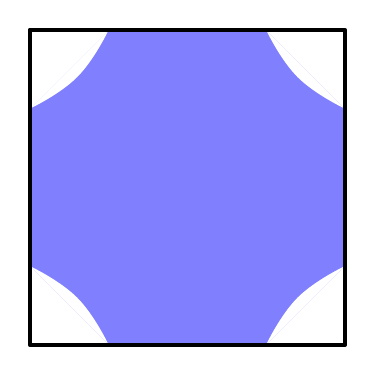
\begin{tikzpicture}[scale=1, font=\footnotesize, line join=round, line cap=round, >=stealth]
\path 	(-1,2) coordinate (A)
(1,2) coordinate (B)
(1,-2) coordinate (E)
(-1,-2) coordinate (G)
(-2,1) coordinate (K)
(2,1) coordinate (C)
(2,-1) coordinate (D)
(-2,-1) coordinate (H);
\fill[blue!50] (-2,2)--(2,2)--(2,-2)--(-2,-2)--cycle;
\fill[white] plot [smooth,tension=0.8] coordinates {(B) (1.4,1.4) (C)};
\fill[white] plot [smooth,tension=0.8] coordinates {(A) (-1.4,1.4) (K)};
\fill[white] plot [smooth,tension=0.8] coordinates {(H) (-1.4,-1.4) (G)};
\fill[white] plot [smooth,tension=0.8] coordinates {(D) (1.4,-1.4) (E)};
\fill[white] (A)--(K)--(-2,2)	(B)--(C)--(2,2) (H)--(-2,-2)--(G) (D)--(2,-2)--(E);
\draw[ultra thick] (-2,2)--(2,2)--(2,-2)--(-2,-2)--cycle;
\end{tikzpicture}\\
\textit{Hình 5}
}
\shortans{$13{,}5$}
\loigiai{
Gắn trục tọạ độ $Oxy$ vào viên gạch sao cho hai trục trùng với hai đường đối xứng, gốc $O$ ở tâm hình vuông như hình dưới. Giả sử tọa độ một điểm nằm trên đường viền cong là $(x;y)$.\\
Theo giả thiết, ta có $|x y|=2$. Suy ra $y=\dfrac{2}{x}$ hoặc $y=\dfrac{-2}{x}$.\\
Ứng với hình dưới, ta có các đường viền cong $AK$, $DE$ là một phần của đồ thị hàm số $y=\dfrac{-2}{x}$; các đường viền cong $BC$, $GH$ là một phần của đồ thị hàm số $y=\dfrac{2}{x}$.
\begin{center}
\begin{tikzpicture}[scale=1, font=\footnotesize, line join=round, line cap=round, >=stealth]
\path 	(-1,2) coordinate (A)
(1,2) coordinate (B)
(1,-2) coordinate (E)
(-1,-2) coordinate (G)
(-2,1) coordinate (K)
(2,1) coordinate (C)
(2,-1) coordinate (D)
(-2,-1) coordinate (H);
\fill[blue!50] (-2,2)--(2,2)--(2,-2)--(-2,-2)--cycle;
\draw[thick,dashed]	(A)--(G)(B)--(E)(K)--(C)(H)--(D);
\fill[white] plot [smooth,tension=0.8] coordinates {(B) (1.4,1.4) (C)};
\fill[white] plot [smooth,tension=0.8] coordinates {(A) (-1.4,1.4) (K)};
\fill[white] plot [smooth,tension=0.8] coordinates {(H) (-1.4,-1.4) (G)};
\fill[white] plot [smooth,tension=0.8] coordinates {(D) (1.4,-1.4) (E)};
\fill[white] (A)--(K)--(-2,2)	(B)--(C)--(2,2) (H)--(-2,-2)--(G) (D)--(2,-2)--(E);
\draw[ultra thick] (-2,2)--(2,2)--(2,-2)--(-2,-2)--cycle;
\draw[->] (-3,0) -- (3,0) node[right] {$x$};
\draw[->] (0,-3) -- (0,3) node[above] {$y$};
\fill (0,2) circle (1pt) node[above left]{$2$};
\fill (0,-2) circle (1pt) node[below left]{$-2$};
\fill (2,0) circle (1pt) node[below right]{$2$};
\fill (-2,0) circle (1pt) node[below left]{$-2$};
\fill (0,0) circle (1pt) node[below left]{$O$};
\foreach \x/\g in {A/90,B/90,C/0,D/0,E/-90,G/-90,H/180,K/180}
\fill[black] 	(\x) circle (1pt)
($(\g:3mm)+(\x)$) node {$\x$};
\end{tikzpicture}
\end{center}
Khi đó, diện tích phần màu xanh bằng
\begin{eqnarray*}
&& \displaystyle\int_{-2}^{-1}\left|\dfrac{-2}{x}-\dfrac{2}{x}\right| \mathrm{\,d} x+\displaystyle\int_1^2\left|\dfrac{2}{x}-\dfrac{-2}{x}\right| \mathrm{\,d} x+S_{ABEG} \\
&=&\displaystyle\int_{-2}^{-1}\left(\dfrac{-2}{x}-\dfrac{2}{x}\right) \mathrm{\,d} x+\displaystyle\int_1^2\left(\dfrac{2}{x}-\dfrac{-2}{x}\right) \mathrm{\,d} x+4\cdot2 \\
&=&-4 \ln |x|\Big|_{-2}^{-1}+4 \ln |x|\Big|_1^2+8 \approx 13{,}5\,\,\left(\mathrm{dm}^2\right).
\end{eqnarray*}
}
\end{ex}

\begin{ex}%[Dự án 2025 - đề cấu trúc mới, Hung Doan]%[2D4C3-1]
Cho hàm số $f(x)=x^3+ax^2+bx+c$ với $a$, $b$, $c$ là các số thực. Biết hàm số $g(x)=f(x)+f'(x)+f'' (x)$ có hai giá trị cực trị là $5$ và $2$. Tính diện tích hình phẳng giới hạn bởi đường $y=\dfrac{f(x)}{g(x)+6}$ và $y=1$, kết quả làm tròn đến hàng phần trăm.
\shortans{$2{,}08$}
\loigiai{
Ta có $f'' '(x)=6$, khi đó $g'(x)=f'(x)+f'' (x)+f'' '(x)=f'(x)+f'' (x)+6$.\\
Giả sử $x_1$, $x_2$ ($x_1<x_2$) là hai điểm cực trị của hàm số $g(x)$.\\
Vì $\lim\limits_{x\to +\infty } g(x)=+\infty $ và $-5$ và $2$ là hai giá trị cực trị của hàm số $g(x)$ nên $\heva{&g(x_1)=2\\&g(x_2)=-5.}$\\
Phương trình hoành độ giao điểm của $y=\dfrac{f(x)}{g(x)+6}$ và $y=1$ là
\begin{align*}
\dfrac{f(x)}{g(x)+6}=1 &\Leftrightarrow g(x)+6=f(x)\\
&\Leftrightarrow f(x)+f'(x)+f'' (x)+6=f(x)\\
&\Leftrightarrow f'(x)+f'' (x)+6=0\\
&\Leftrightarrow \hoac{&x=x_1\\&x=x_2.}
\end{align*}
Khi đó diện tích hình phẳng cần tìm là
\begin{align*}
S&=\displaystyle\int \limits_{x_1}^{x_2} \left|\dfrac{f(x)}{g(x)+6}-1\right|\mathrm{d}x\\
&=\left|\displaystyle\int \limits_{x_1}^{x_2} \dfrac{f'(x)+f'' (x)+6}{g(x)+6}\mathrm{d}x\right|\\
&=\left|\displaystyle\int \limits_{x_1}^{x_2} \dfrac{g'(x)}{g(x)+6}\mathrm{d}x\right|\\
&=\left|\ln |g(x)+6|\bigg|_{x_1}^{x_2}\right| \\
&=\left|\ln |g(x_2)+6|-\ln |g(x_1)+6|\right|\\
&=\ln 8\approx 2{,}08.
\end{align*}
}
\end{ex}

\begin{ex}%[Dự án 2025 - đề cấu trúc mới, Nguyễn Kiều Nhã Tú]%[2D4C3-1]
Cho parabol $(P)\colon y=x^2$ có hai điểm $A(x_1;y_1)$, $B(x_2;y_2)\in (P)$ sao cho $AB=4$ và diện tích hình phẳng giới hạn bởi $(P)$ và đường thẳng $AB$ đạt giá trị lớn nhất. Tính giá trị của biểu thức $T=x_1+x_2+y_1+y_2$.
\shortans{$8$}
\loigiai{
\immini{
Gọi $A(a;a^2)$ và $B(b;b^2)\in (P)$ với $a<b$.\\
Khi đó ta có phương trình đường thẳng $AB$ là $y=(a+b)x-ab$.\\
$S=\displaystyle\int\limits_a^b ((a+b)x-ab-x^2)\mathrm{\,d}x= \dfrac{1}{6}(b-a)^3$.\\
Mà $0<b-a\le AB=4 \Rightarrow S=\dfrac{1}{6}(b-a)^3 \le \dfrac{32}{3}$.
}
{
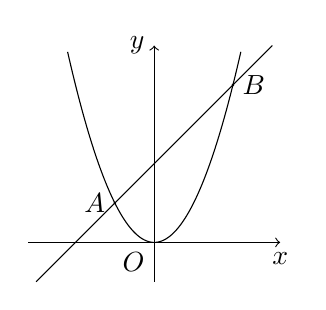
\begin{tikzpicture}[scale=0.5]
\def\a{1}
\def\b{0}
\def\c{0}
\def\f(#1){\a*((#1)^2)+\b*(#1)+\c}
\def\xmin{-2.2}
\def\xmax{2.2}
\def\ymin{-1}
\def\ymax{4}
\draw[->] (\xmin-1,0)--(\xmax+1,0) node[below] {$x$};
\draw[->] (0,\ymin)--(0,\ymax+1) node[left]{$y$};
\draw (0,0) node [below left] {$O$};
\draw (-3,-1)--(-2,0)--(-1,1)node[ left]{$A$}--(2,4)node[right]{$B$} --(3,5);
\fill (-1,1) circle(1pt) (2,4) circle(1pt);
\draw[smooth,samples=200] plot[domain=\xmin:\xmax]  (\x,{\f(\x)});
\clip (\xmin,\ymin) rectangle (\xmax,\ymax);
\end{tikzpicture}}
\begin{align*}
S_{\max}=\dfrac{32}{3}&\Leftrightarrow \heva{&b-a=4\\&AB=4} \Leftrightarrow \heva{&b-a=4\\&(b-a)^2+(b^2-a^2)=16}\\
&\Leftrightarrow \heva{&b-a=4\\&b^2-a^2=0}\Leftrightarrow\heva{&b-a=4\\&b+a=0} \Leftrightarrow \heva{&b=2\\&a=-2.}
\end{align*}
Suy ra $A(-2;4)$, $B(2;4)$. Vậy $T=8$.
}
\end{ex}

\begin{ex}%[Dự án 2025 - đề cấu trúc mới, Nguyễn Kiều Nhã Tú]%[2D4C3-1]
Cho hàm số $y=x^2-4x+3$ có đồ thị là parabol $(P)$ và điểm $M(3;2)$. Gọi $d$ là đường thẳng đi qua điểm $M$ và $S$ là diện tích hình phẳng được giới hạn bởi đường thẳng $d$ và parabol $(P)$. Biết rằng $S_{\min}=\dfrac{a\sqrt{2}}{b}$ với $a$, $b\in \mathbb{Z}^+$ và $\dfrac{a}{b}$ tối giản. Tính giá trị biểu thức $2a^3+3b^3$.
\shortans{$1105$}
\loigiai{
Đường thẳng $d$ đi qua $M(3;2)$ có hệ số góc là $k$ nên $d\colon y=k(x-3)+2$.\\
Phương trình hoành độ giao điểm của $d$ và $(P)$ là\\ $x^2-4x+3=k(x-3)+2 \Leftrightarrow x^2-(k+4)x+3k+1=0. \quad(1)$\\
$\Delta=(k+4)^2-4(3k+1)=k^2-4k+12=(k-2)^2+8>0$, $\forall k\in \mathbb{R}$.\\
Phương trình $(1)$ luôn có hai nghiệm phân biệt $x_1$, $x_2$, giả sử $x_1<x_2$, ta có $\heva{&x_1+x_2=k+4\\&x_1x_2=3k+1.}$\\
Diện tích hình phẳng giới hạn bởi $(P)$ và $d$ là
\begin{align*}
S&=\displaystyle\int\limits_{x_1}^{x_2} \left|x^2-(k+4)x+3k+1\right| \mathrm{\,d}x = \Big[ \dfrac{(k+4)x^2}{2}-\dfrac{x^3}{3}-(3k+1)x \Big]\Big|_{x_1}^{x_2}\\
&=\dfrac{k+4}{2}\Big(x_2^2-x_1^2\Big)-\dfrac{1}{3}\Big(x_2^3-x_1^3\Big)-(3k+1)(x_2-x_1)\\
&=(x_2-x_1)\left[ \dfrac{(k+4)(x_2+x_1)}{2}-\dfrac{(x_2+x_1)^2-x_1x_2}{3}-(3k+1) \right]\\
&=\dfrac{1}{6}\sqrt{(x_2+x_1)^2-4x_1x_2} \Big[3(k+4)(x_2+x_1)-2(x_2+x_1)^2+2x_1x_2-6(3k+1)\Big]\\
&=\dfrac{1}{6}\sqrt{(k+4)^2-4(3k+1)}\Big[(k+4)^2-4(3k+1)\Big]\\
&=\dfrac{1}{6}\sqrt{(k-2)^2+8}\Big[(k-2)^2+8\Big]\ge \dfrac{8\sqrt{2}}{3}.
\end{align*}
Do đó $S_{\min}=\dfrac{8\sqrt{2}}{3}$ đạt được khi $k=2$.\\
Vậy $a=8$, $b=3$ nên $2a^3+3b^3=1105$.
}
\end{ex}

\begin{ex}%[TT-THPT-Trần Đại Nghĩa-Đề 2-Đồng Nai-NH24-25-TN]%[Dự Án C-Đợt 2-Nguyễn Chiến]%[2D4C3-1]
\immini[thm]{
Người ta thiết kế một mẫu gạch lát nền nhà có dạng hình vuông cạnh $4$ (dm). Bốn góc viên gạch màu trắng, phần ở giữa màu xanh như hình vẽ bên. Đường viền của phần màu xanh bao gồm bốn đoạn thẳng nằm trên các cạnh hình vuông và bốn đường cong có tính chất: Tích khoảng cách từ một điểm bất kì thuộc đường cong đó đến hai trục đối xứng của viên gạch (hai đường thẳng đi qua tâm viên gạch và lần lượt song song với hai cạnh vuông góc) bằng $2$ $\left(\text{dm}^2\right)$. Hãy cho biết phần màu xanh có diện tích bằng bao nhiêu đề-xi-mét vuông? (\textit{Làm tròn kết quả đến hàng phần mười}).
}{
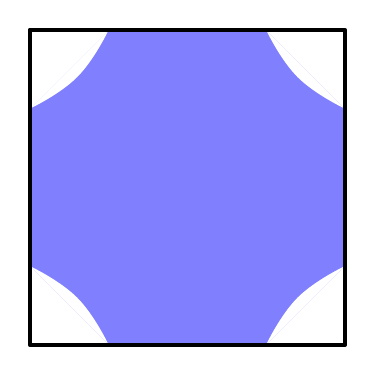
\begin{tikzpicture}[scale=1, font=\footnotesize, line join=round, line cap=round, >=stealth]
\path 	(-1,2) coordinate (A)
(1,2) coordinate (B)
(1,-2) coordinate (E)
(-1,-2) coordinate (G)
(-2,1) coordinate (K)
(2,1) coordinate (C)
(2,-1) coordinate (D)
(-2,-1) coordinate (H);
\fill[blue!50] (-2,2)--(2,2)--(2,-2)--(-2,-2)--cycle;
\fill[white] plot [smooth,tension=0.8] coordinates {(B) (1.4,1.4) (C)};
\fill[white] plot [smooth,tension=0.8] coordinates {(A) (-1.4,1.4) (K)};
\fill[white] plot [smooth,tension=0.8] coordinates {(H) (-1.4,-1.4) (G)};
\fill[white] plot [smooth,tension=0.8] coordinates {(D) (1.4,-1.4) (E)};
\fill[white] (A)--(K)--(-2,2)	(B)--(C)--(2,2) (H)--(-2,-2)--(G) (D)--(2,-2)--(E);
\draw[ultra thick] (-2,2)--(2,2)--(2,-2)--(-2,-2)--cycle;
\end{tikzpicture}
}
\par\shortans[0]{13{,}5}
\loigiai{
Gắn trục tọạ độ $Oxy$ vào viên gạch sao cho hai trục trùng với hai đường đối xứng (đơn vị trên mỗi trục là dm), gốc $O$ ở tâm hình vuông như hình dưới. Giả sử tọa độ một điểm nằm trên đường viền cong là $(x;y)$.\\
Theo giả thiết, ta có $|x y|=2$. Suy ra $y=\dfrac{2}{x}$ hoặc $y=\dfrac{-2}{x}$.\\
Ứng với hình dưới, ta có các đường viền cong $AK$, $DE$ là một phần của đồ thị hàm số $y=\dfrac{-2}{x}$; các đường viền cong $BC$, $GH$ là một phần của đồ thị hàm số $y=\dfrac{2}{x}$.
\immini{Khi đó, diện tích phần màu xanh bằng
\begin{eqnarray*}
&& \displaystyle\int\limits_{-2}^{-1}\left|\dfrac{-2}{x}-\dfrac{2}{x}\right|\,\mathrm{d}x+\displaystyle\int\limits_1^2\left|\dfrac{2}{x}-\dfrac{-2}{x}\right|\,\mathrm{d}x+S_{ABEG} \\
&=&\displaystyle\int\limits_{-2}^{-1}\left(\dfrac{-2}{x}-\dfrac{2}{x}\right)\,\mathrm{d}x+\displaystyle\int\limits_1^2\left(\dfrac{2}{x}-\dfrac{-2}{x}\right)\,\mathrm{d}x+4\cdot2 \\
&=&-4 \ln |x|\Big|_{-2}^{-1}+4 \ln |x|\Big|_1^2+8 \approx 13{,}5\,\,\left(\text{dm}^2\right).
\end{eqnarray*}}{\begin{tikzpicture}[scale=1, font=\footnotesize, line join=round, line cap=round, >=stealth]
\path 	(-1,2) coordinate (A)
(1,2) coordinate (B)
(1,-2) coordinate (E)
(-1,-2) coordinate (G)
(-2,1) coordinate (K)
(2,1) coordinate (C)
(2,-1) coordinate (D)
(-2,-1) coordinate (H);
\fill[blue!50] (-2,2)--(2,2)--(2,-2)--(-2,-2)--cycle;
\draw[thick,dashed]	(A)--(G)(B)--(E)(K)--(C)(H)--(D);
\fill[white] plot [smooth,tension=0.8] coordinates {(B) (1.4,1.4) (C)};
\fill[white] plot [smooth,tension=0.8] coordinates {(A) (-1.4,1.4) (K)};
\fill[white] plot [smooth,tension=0.8] coordinates {(H) (-1.4,-1.4) (G)};
\fill[white] plot [smooth,tension=0.8] coordinates {(D) (1.4,-1.4) (E)};
\fill[white] (A)--(K)--(-2,2)	(B)--(C)--(2,2) (H)--(-2,-2)--(G) (D)--(2,-2)--(E);
\draw[ultra thick] (-2,2)--(2,2)--(2,-2)--(-2,-2)--cycle;
\draw[->] (-3,0) -- (3,0) node[right] {$x$};
\draw[->] (0,-3) -- (0,3) node[above] {$y$};
\fill (0,2) circle (1pt) node[above left]{$2$};
\fill (0,-2) circle (1pt) node[below left]{$-2$};
\fill (2,0) circle (1pt) node[below right]{$2$};
\fill (-2,0) circle (1pt) node[below left]{$-2$};
\fill (0,0) circle (1pt) node[below left]{$O$};
\foreach \x/\g in {A/90,B/90,C/0,D/0,E/-90,G/-90,H/180,K/180}
\fill[black] 	(\x) circle (1pt)
($(\g:3mm)+(\x)$) node {$\x$};
\end{tikzpicture}}
}
\end{ex}

\begin{ex}%[ST12-dot1-Trần xuân Hòa]%[2D4C3-2]
\immini{Một hoa văn trang trí được tạo ra từ một miếng bìa hình vuông cạnh bằng $10$ cm bằng cách khoét đi bốn phần bằng nhau có hình dạng parabol như hình vẽ bên. Biết $ AB=5$ cm, $OH=4$ cm. Tính diện tích của bề mặt hoa văn đó (đơn vị: cm$^2$) (kết quả làm tròn đến chữ số thập phân thứ nhất).
\shortans{$46{,}7$}
}{\begin{tikzpicture}[scale=0.9, font=\footnotesize, line join=round, line cap=round,>=stealth]
\tikzset{label style/.style={font=\footnotesize}}
\def \r{0.5*sqrt(3)};
\coordinate (A) at ($(2,{\r})$);
\coordinate (B) at ($(2,{-\r})$);
\coordinate (H) at ($(A)!0.5!(B)$);
\clip(-2,-2) rectangle (2.5,2);
\fill [black] (-2,-2) rectangle (2,2);
\foreach \i in {0,90,180,270}
\draw [rotate=\i, fill=white,smooth, samples=200]  plot [domain={-\r-0.01}:{\r+0.01}] (\x, {2*(\x)^2+0.5});
\draw (A) node[right]{$ A $}--(B)node[right]{$ B $};
\draw (0.5, 0) node[left]{$\color{white} O $}--(H)node[right]{$H$};
\end{tikzpicture}}
\loigiai{
Diện tích bề mặt hoa văn là $ S=10^2-4S_0 $, trong đó $ S_0 $ là diện tích của Parabol.
\immini{Chọn hệ trục tọa độ như hình vẽ bên.\\
Parabol có đỉnh $ O(0; 0) $ và đi qua điểm $ B\left(\dfrac{5}{2}; 4\right) $ nên có phương trình là $ y=\dfrac{16}{25}x^2 $.\\
Tính $S_0$. Ta có $S_0=4\cdot 5-2\cdot \displaystyle\int\limits_{0}^{\tfrac{5}{2}}\dfrac{16}{25}x^2\mathrm{\, d}x=\dfrac{40}{3}$ (cm$^2$).
}{
\begin{tikzpicture}[scale=0.7, font=\footnotesize, line join=round, line cap=round,>=stealth]
\def \xmin{-3.1}
\def \xmax{3.1}
\def \ymin{-1.9}
\def \ymax{5.3}
\draw[->] (\xmin, 0.) -- (\xmax,0.) node[anchor=north] {$x$};
\draw[->] (0.,\ymin) -- (0.,\ymax) node[anchor=west] {$y$};
\clip(\xmin,\ymin) rectangle (\xmax,\ymax);
\draw[smooth,samples=100,domain=\xmin:\xmax] plot(\x,{0.64*(\x)^2});
\draw[pattern=north west lines,smooth,samples=100,domain=-2.5:2.5] plot(\x,{0.64*(\x)^2});
\draw[dashed] (-2.5,0) node[below] {$-\dfrac{5}{2}$} -- (-2.5,4)node[left]{$ A $}--(0,4)node[above left] {$4$}--(2.5,4)node[right]{$ B $}--(2.5,0)node[below]{$ \dfrac{5}{2} $};
\draw(0,4)node[above right]{$ H $};
\draw[fill=black] (0,0) circle (1.5pt) node[below left] {$O$};
\end{tikzpicture}}\noindent
Vậy diện tích bề mặt hoa văn là $ S=100-4\cdot\dfrac{40}{3}=\dfrac{140}{3}\approx 46{,}7$ (cm$^2$).
}
\end{ex}

\begin{ex}%[2D4C3-2]
\immini
{Ông An xây dựng một sân bóng đá mini hình chữ nhật có chiều rộng $30$m và chiều dài $50$m. Để giảm bớt chi phí cho việc trồng cỏ nhân tạo, ông An chia sân bóng ra làm hai phần (tô đen và không tô đen) như hình bên. Phần tô đen gồm hai phần diện tích bằng nhau và đường cong $AIB$ là một parabol đỉnh $I$ được trồng cỏ nhân tạo với giá $130\,000$ đồng/m$^2$ và phần còn lại được trồng với giá $90\,000$ đồng/m$^2$.
}
{\begin{tikzpicture}[scale=0.9, font=\footnotesize,line join=round, line cap=round, >=stealth]
\coordinate (I) at (0,0);
\coordinate (A) at (1.5,2.25);
\coordinate (B) at ($(A)+(0,-4.5)$);
\coordinate (C) at ($(B)+(-7.5,0)$);
\coordinate (D) at ($(A)-(B)+(C)$);
\coordinate (M) at ($(A)!1/2!(D)$);
\coordinate (N) at ($(B)!1/2!(C)$);
\coordinate (P) at ($(A)+(-1.5,0)$);
\coordinate (Q) at ($(B)+(-1.5,0)$);
\coordinate (R) at ($(D)+(1.5,0)$);
\coordinate (S) at ($(C)+(1.5,0)$);
\coordinate (td) at ($(D)+(0,0.3)$);
\coordinate (dt) at ($(D)+(-0.3,0)$);
\coordinate (ct) at ($(C)+(-0.3,0)$);
\coordinate (tr) at ($(R)+(0,0.3)$);
\coordinate (rp) at ($(R)+(0.3,0)$);
\coordinate (I') at ($(R)!1/2!(S)$);
\coordinate (g) at ($(I')+(0.3,0)$);
\fill[gray]plot[domain=0:1.5](\x,{sqrt(3.375*(\x))})--(A)--plot[domain=1.5:0](\x,{-sqrt(3.375*(\x))})--cycle;
\fill[gray](C)--(D)--plot[domain=-6:-4.5](\x,{sqrt(3.375*(-\x-4.5))})--plot[domain=-4.5:-6](\x,{-sqrt(3.375*(-\x-4.5))})--cycle;
\draw (A)--(B)--(C)--(D)--cycle (M)--(N);
\draw[dashed] (P)--(Q) (R)--(S);
\draw[<->](td)--(tr);
\node at ($(td)!1/2!(tr)$)[above]{$10$ m};
\draw[<->](dt)--(ct);
\node at ($(dt)!1/2!(ct)$)[above,rotate=90]{$30$ m};
\draw[<->](rp)--(g);
\node at ($(rp)!1/2!(g)$)[above,rotate=-90]{$15$ m};
\foreach \x/\g in {A/90,B/-90,I/180,I'/-40}\draw[fill=black] (\x) circle (.05) +(\g:.5)node{\footnotesize$\x$};
\end{tikzpicture}}
\noindent
Hỏi ông An phải trả bao nhiêu tiền (triệu đồng) để trồng cỏ nhân tạo cho sân bóng.
\shortans{$151$}
\loigiai{
\immini{
Chọn hệ trục tọa độ như hình vẽ ($I$ là gốc tọa độ). Khi đó đường cong $IAB$ là một parabol có phương trình dạng $y=ax^2$.\\
Parabol đi qua điểm $\left(15;10 \right)$, suy ra
\[a \cdot 15^2=10 \Rightarrow a=\dfrac{2}{45}.\]
}
{
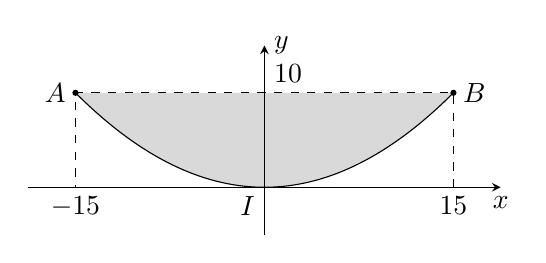
\begin{tikzpicture}[smooth,samples=300,scale=0.6,>=stealth]
\fill[gray!30] (-4,2)--(4,2)--plot[domain=4:-4](\x,{0.125*(\x)^2});
\draw[->] (-5,0)--(5,0) node[below]{$x$};
\draw[->] (0,-1)--(0,3) node[right]{$y$};
\draw (0,0) node[below left]{$I$};
\draw[domain=-4:4] plot(\x,{0.125*(\x)^2});
\draw[fill=black] (4,2) circle(1.5pt) (-4,2) circle(1.5pt);
\draw[dashed] (4,0)node[below]{$15$}--(4,2)node[right]{$B$}--(-4,2)node[left]{$A$}--(-4,0)node[below]{$-15$};

\node[right] at (0,2.4) {$10$};
\end{tikzpicture}}
\noindent
Vậy $y=\dfrac{2}{45}x^2$. Diện tích phần tô đen là $S=2 \cdot \displaystyle\int\limits_{-15}^{15} \left(10-\dfrac{2}{45}x^2 \right) \mathrm{\,d}x=400 \, (\text{m}^2)$.\\
Diện tích phần còn lại của sân bóng là $S_2=30 \cdot 50-400=1100\,(\text{m}^2).$\\
Số tiền Ông An phải trả để trồng cỏ nhân tạo cho sân bóng là
\[130000\times 400+90000\times 1100=151000000\text{ đồng}=151\text{ triệu đồng.}\]}
\end{ex}

\begin{ex}%[12-MH-2-MH2025]%[MH-2025, Nguyễn Trần Phong]%[2D4C3-2]
\immini{Chướng ngại vật \lq\lq tường cong\rq\rq trong một sân thi đấu X-Game là một khối bê tông có chiều cao từ mặt đất lên là $3$ m. Giao của mặt tường cong và mặt đất là đoạn thẳng $AB = 2$ m. Thiết diện của khối tường cong cắt bởi mặt phẳng vuông góc với $AB$ tại $A$ là một hình tam giác vuông cong $ACE$ với $AC = 4$ m, $CE = 3$ m và cạnh cong $AE$ nằm trên một đường Parabol có trục đối xứng vuông góc với mặt đất. Tại vị trí $M$ là trung điểm của $AC$ thì tường cong có độ cao $1$ m. Thể tích bê tông cần sử dụng để tạo nên khối tường cong đó gần nhất với số nào dưới đây?
\shortans{$9{,}3$}
}{\begin{tikzpicture}[>=stealth,x=0.8cm,y=0.8cm,scale=0.7]
\coordinate[label=below:$A$] (A) at (0,0);
\coordinate[label=left:$B$] (B) at (-2,2);
\coordinate[label=below:$C$] (C) at (6,0);
\coordinate[label=right:$E$] (E) at (6,6);
\coordinate (G) at (2,4);
\coordinate (H) at (4,1.8);
\coordinate (D) at ($(C)+(B)-(A)$);
\coordinate (F) at ($(E)+(D)-(C)$);
\coordinate[label=below:$M$] (M) at ($(A)!0.5!(C)$);
\coordinate (K) at ($(A)!0.5!(B)$);
\coordinate (N) at ($(M)+(0,1.1)$);
\draw (D)--(C)--(A)--(B) (C)--(E)--(F) (M)--(N);
\draw[dashed] (B)--(D)--(F);
\foreach \diem in {A,B,C,D,E,F,M,F}	\fill (\diem)circle(1.5pt);
%\tkzLabelPoints[above left](D)
%\tkzLabelSegment[right](M,N){\footnotesize$1$ m}
%\tkzLabelSegment[left](A,B){\footnotesize$2$ m}
%\tkzLabelSegment[right](C,E){\footnotesize$3{,}5$ m}
\draw(-1,.8) node[left]{\footnotesize $2$ m} (3,0.8) node[right]{\footnotesize$1$ m} (6,3) node[right]{\footnotesize$3$ m};

\draw plot[smooth,tension=.65] coordinates{(B) (G) (F)};
\draw plot[smooth,tension=.65] coordinates{(A) (H) (E)};
\fill [pattern = north east lines] plot[smooth,tension=.65] coordinates{(A) (H) (E)} (0,0) --(-2,2)--(4,8)--(6,6)--cycle;
\fill [draw=none, pattern = north east lines, color=white] (0,0) plot[smooth,tension=.65] coordinates{(B) (G) (F)} (-2,2)--(4,2)--cycle;
\end{tikzpicture}
}
\loigiai{
\immini{Chọn hệ trục tọa độ như hình vẽ.\\
Gọi $AE \colon y = ax^2 + bx + c$.\\
Do $AE$ đi qua $A(-4; 0)$ nên ta có $16a - 4b + c = 0$.\\
Do $E (0; 3)$ thuộc cạnh cong $AE$ nên $c = 3$ (2).\\
Do $N(-2; 1)$ thuộc cạnh cong $AE$ nên $4a - 2b + c = 1$ (3).\\
Từ (1), (2), (3) suy ra $a = \dfrac{1}{8}$, $b = \dfrac{5}{4}$, $c = 3 \Rightarrow AE \colon y = \dfrac{1}{8}x^2 + \dfrac{5}{4}x + 3$.\\
Khi đó $S_{AEC} = \displaystyle\int_{-4}^0\left(\dfrac{1}{8} x^2 + \dfrac{5}{4}x + 3\right) dx = \dfrac{14}{3}\left(m^2\right)$.
}{\begin{tikzpicture}[>=stealth,x=0.8cm,y=0.8cm,scale=0.7]
\coordinate[label=below:$A$] (A) at (0,0);
\coordinate[label=left:$B$] (B) at (-2,2);
\coordinate[label=below:$C$] (C) at (6,0);
\coordinate[label=right:$E$] (E) at (6,6);
\coordinate (G) at (2,4);
\coordinate (H) at (4,1.8);
\coordinate[label = above left:$D$] (D) at ($(C)+(B)-(A)$);
\coordinate[label = above:$F$] (F) at ($(E)+(D)-(C)$);
\coordinate[label=below:$M$] (M) at ($(A)!0.5!(C)$);
\coordinate (K) at ($(A)!0.5!(B)$);
\coordinate[label=above left:$N$] (N) at ($(M)+(0,1.1)$);
\draw (D)--(C)--(A)--(B) (C)--(E)--(F) (M)--(N);
\draw[dashed] (B)--(D) (D)--(F);
\foreach \diem in {A,B,C,D,E,F,M,F,N}	\fill (\diem)circle(1.5pt);
\coordinate (x) at ($(M)!1.5!(C)$);
\draw[->](C)--(x); \draw (x) node[right]{$x$};
\coordinate (y) at ($(C)!1.4!(E)$);
\draw[->](E)--(y); \draw (y) node[right]{$y$};
%\tkzLabelPoints[above left](D)
%\tkzLabelSegment[right](M,N){\footnotesize$1$ m}
%\tkzLabelSegment[left](A,B){\footnotesize$2$ m}
%\tkzLabelSegment[right](C,E){\footnotesize$3{,}5$ m}
\draw plot[smooth,tension=.65] coordinates{(B) (G) (F)};
\draw plot[smooth,tension=.65] coordinates{(A) (H) (E)};
\fill [pattern = north east lines] plot[smooth,tension=.65] coordinates{(A) (H) (E)} (0,0) --(-2,2)--(4,8)--(6,6)--cycle;
\fill [draw=none, pattern = north east lines, color=white] (0,0) plot[smooth,tension=.65] coordinates{(B) (G) (F)} (-2,2)--(4,2)--cycle;
\end{tikzpicture}
}
\noindent Thể tích khối tường cong là $V = S_{AEC} \cdot AB = \frac{14}{3} \cdot 2 = \dfrac{28}{3} = 9{,}3\left(\mathrm{~m}^3\right)$.	}
\end{ex}

\begin{ex}%[EX-Ôn Tập TN 2025, Võ Thanh Phong]%[2D4C3-2]
Một cổng có đạng hình parabol với chiều cao $8$ m, chiều rộng chân đế $8$ m. Người ta căng hai sợi dây trang trí $AB$,  $CD$ nằm ngang, đồng thời chia cổng thành ba phần sao cho hai phần ở phía trên có diện tích bằng nhau. Tỉ số $\dfrac{CD}{AB}$ bằng bao nhiêu (làm tròn kết quả đến hàng phần trăm)?
\begin{center}
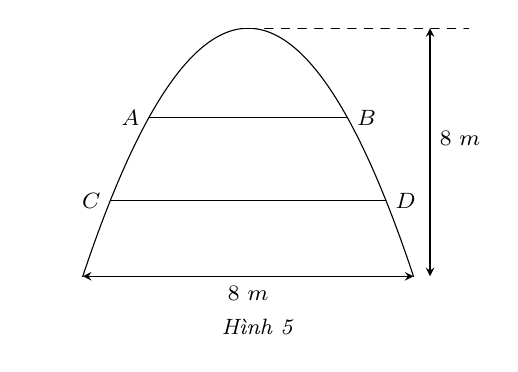
\begin{tikzpicture}[scale=0.7, font=\footnotesize, line join=round, line cap=round,>=stealth]
\begin{scope}
\clip (-4,-4.5) rectangle (4,0);
\draw [smooth,domain=-5:4, samples=200] plot (\x, {-0.5*(\x)^2});
\end{scope}
\draw [<->] (3.3,0)--(3.3,-4.5);
\node[right] at (3.3,-2){$8\,\,m$};
\draw [<->] (-3,-4.5)--(3,-4.5);
\node[below] at (0,-4.5){$8\,\,m$};
\node[left] at (-1.8,-1.62){$A$};
\node[right] at (1.8,-1.62){$B$};
\node[left] at (-2.5,-3.125){$C$};
\node[right] at (2.5,0-3.125){$D$};
\draw [-] (-1.8,-1.62)--(1.8,-1.62);
\draw [-] (-2.5,-3.125)--(2.5,0-3.125);
\draw [dashed] (0,0)--(4,0);
\node[below] at (current bounding box.south){\textit{Hình 5}};
\end{tikzpicture}
\end{center}
\shortans{ $1{,}26$                 }
\loigiai{
\immini{Gắn hệ trục tọa độ $Oxy$ vào cổng parabol như hình bên với trục $Oy$ trùng với đường đối xứng của parabol, gốc $O$ nằm ở đỉnh của parabol, đơn vị trên mỗi trục tính theo mét. Khi đó, phương trình parabol có dạng $y=ax^2$.\\
Vì parabol đi qua điểm có toạ độ $(-4 ;-8)$ nên $a=-\dfrac{1}{2}$. Suy ra phương trình parabol là $y=-\dfrac{1}{2} x^2$.\\}{
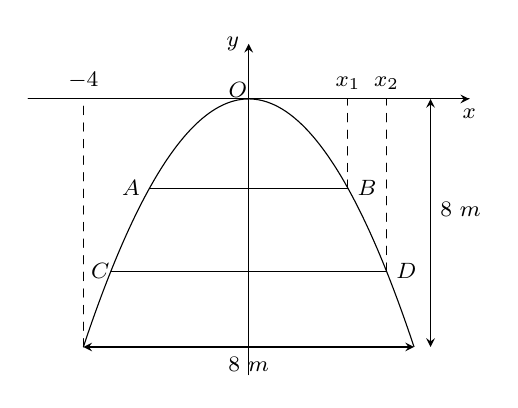
\begin{tikzpicture}[scale=0.7, font=\footnotesize, line join=round, line cap=round,>=stealth]
\draw[->] (-4,0) --(4,0) node[below]{$x$};
\draw[->] (0,-5) --(0,1) node[left]{$y$};
\draw (0,0) node[above left=-3pt]{$O$};
\begin{scope}
\clip (-4,-4.5) rectangle (4,0);
\draw [smooth,domain=-5:4, samples=200] plot (\x, {-0.5*(\x)^2});
\end{scope}
\draw [<->] (3.3,0)--(3.3,-4.5);
\node[right] at (3.3,-2){$8\,\,m$};
\draw [<->] (-3,-4.5)--(3,-4.5);
\node[below] at (0,-4.5){$8\,\,m$};
\node[left] at (-1.8,-1.62){$A$};
\node[right] at (1.8,-1.62){$B$};
\node[left=-3pt] at (-2.5,-3.125){$C$};
\node[right] at (2.5,0-3.125){$D$};
\draw [-] (-1.8,-1.62)--(1.8,-1.62);
\draw [-] (-2.5,-3.125)--(2.5,0-3.125);
\draw [dashed] (0,0)--(4,0) (1.8,-1.62)--(1.8,0) (2.5,0-3.125)--(2.5,0) (-3,-4.5)--(-3,0);
\node[above] at (1.8,0){$x_1$};
\node[above] at (2.5,0){$x_2$};
\node[above] at (-3,0){$-4$};
\end{tikzpicture}}
Giả sử $B$ có hoành độ $x_1$,  $D$ có hoành độ $x_2$. Khi đó, phương trình đường thẳng $AB$ là $y=-\dfrac{1}{2} x_1^2$, phương trình đường thẳng $CD$ là $y=-\dfrac{1}{2} x_2^2$.\\
Diện tích hình phẳng giới hạn bởi parabol và đường thẳng $AB$ là
\[
S_1=2\displaystyle\int\limits_0^{x_1}\left[-\dfrac 12x^2-\left(-\dfrac 12x_1^2\right)\right]\mathrm{\,d} x=\left.2\left(-\dfrac{x^3}6+\dfrac{x_1^2}2x\right)\right|_0^{x_1}=\dfrac 23x_1^3\,\,\left(\mathrm{m}^2\right).
\]
Diện tích hình phẳng giới hạn bởi parabol và đường thẳng $CD$ là
\[
S_2=2\displaystyle\int\limits_0^{x_2}\left[-\dfrac 12x^2-\left(-\dfrac 12x_2^2\right)\right]\mathrm{\,d} x=\left.2\left(-\dfrac{x^3}6+\dfrac{x_2^2}2x\right)\right|_0^{x_2}=\dfrac 23x_2^3\,\,\left(\mathrm{m}^2\right).
\]
Theo giả thiết, ta có  $S_2=2S_1\Leftrightarrow x_2^3=2x_1^3\Leftrightarrow\dfrac{x_2}{x_1}=\sqrt[3]2\approx 1{,}26$.\\
Khi đó, $\dfrac{CD}{AB}=\dfrac{2x_2}{2x_1}\approx 1{,}26$.
}
\end{ex}

\begin{ex}%[Dự án 2025 - đề cấu trúc mới, Hung Doan]%[2D4C3-2]
\immini[thm]{Một bức tường lớn kích thức $8$m $\times$ $8$m trước đại sảnh của một tòa biệt thự được sơn các loại sơn đặc biệt. Người ta vẽ hai nửa đường tròn đường kính $AD$, $AB$ cắt nhau tại $H$; đường tròn tâm $D$, bán kính $AD$, cắt nửa đường tròn đường kính $AB$ tại $K$. Biết tam giác cong $AHK$ được sơn màu xanh và các phần còn lại được sơn màu trắng (như hình vẽ) và một mét vuông sơn trắng, sơn xanh lần lượt có giá là $1$ triệu đồng và $1{,}5$ triệu đồng. Số tiền phải trả là bao nhiêu triệu đồng? (làm tròn đến hàng triệu).}{
\begin{tikzpicture}[scale=1, font=\footnotesize, line join=round, line cap=round, >=stealth]
\begin{scope}
\clip (0,0) rectangle (4,4);
\fill[pattern=north east lines,smooth] (0,0)--plot[domain=0:4](\x,{sqrt(16-(\x)^2)})--(4,0)--cycle;
\fill[white,smooth] (0,0)--plot[domain=0:4](\x,{4-sqrt(4*(\x)-(\x)^2)})--(4,0)--cycle;
\draw[fill=white,samples=200,domain=0:4,smooth] (0,2) circle (2);
\draw[samples=200,domain=0:4,smooth,variable=\x] plot (\x,{sqrt(16-(\x)^2)});
\draw[samples=200,domain=0:4,smooth,variable=\x] plot (\x,{4-sqrt(4*(\x)-(\x)^2)});
%\draw[samples=200,domain=0:4,smooth] (0,2) circle (2);
\end{scope}
\draw (0,0)rectangle (4,4);
\node at (0, 2) [left]{$8$};
\node at (2,0) [below]{$8$};
\fill (0,4) node[above left]{$A$} circle(1pt);
\fill (0,0) node[below left]{$B$} circle(1pt);
\fill (4,0) node[below right]{$C$} circle(1pt);
\fill (4,4) node[above right]{$D$} circle(1pt);
\fill (2,2) node[below left]{$H$} circle(1pt);
\fill (3.2,2.4) node[below]{$K$} circle(1pt);
\draw (0,0)rectangle (0.2,0.2);
\draw (0,4)rectangle (0.2,3.8);
\draw (4,0)rectangle (3.8,0.2);
\draw (4,4)rectangle (3.8,3.8);
\end{tikzpicture}
}
\shortans{$67$}
\loigiai{
Chọn hệ toạ độ ${Oxy}$ như hình vẽ sau
\begin{center}
\begin{tikzpicture}[scale=1, font=\footnotesize, line join=round, line cap=round, >=stealth]
\begin{scope}
\clip (0,0) rectangle (4,4);
\fill[pattern=north east lines,smooth] (0,0)--plot[domain=0:4](\x,{sqrt(16-(\x)^2)})--(4,0)--cycle;
\fill[white,smooth] (0,0)--plot[domain=0:4](\x,{4-sqrt(4*(\x)-(\x)^2)})--(4,0)--cycle;
\draw[fill=white,samples=200,domain=0:4,smooth] (0,2) circle (2);
\draw[samples=200,domain=0:4,smooth,variable=\x] plot (\x,{sqrt(16-(\x)^2)});
\draw[samples=200,domain=0:4,smooth,variable=\x] plot (\x,{4-sqrt(4*(\x)-(\x)^2)});
%\draw[samples=200,domain=0:4,smooth] (0,2) circle (2);
\end{scope}
\draw (0,0)rectangle (4,4);
\node at (0, 2) [left]{$8$};
\node at (2,0) [below]{$8$};
\fill (0,4) node[above left]{$A$} circle(1pt);
\fill (0,0) node[below left]{$B$} circle(1pt);
\fill (4,0) node[below right]{$C$} circle(1pt);
\fill (4,4) node[above right]{$D$} circle(1pt);
\fill (2,2) node[below left]{$H$} circle(1pt);
\fill (3.2,2.4) node[below]{$K$} circle(1pt);
\draw (0,0)rectangle (0.2,0.2);
\draw (0,4)rectangle (0.2,3.8);
\draw (4,0)rectangle (3.8,0.2);
\draw (4,4)rectangle (3.8,3.8);
\draw[->](-0.5, 0)--(5, 0) node[below]{$x$};
\draw[->](0,-0.5)--(0,5) node[left]{$y$};
\node at (0, 0) [above left]{$O$};
\draw[dashed] (2,2)--(2,3.4641)node[above]{$E$};
\end{tikzpicture}
\end{center}
Dễ thấy cung $AB$ có phương trình $y=f(x)=8-\sqrt{16-(x-4)^2}$; cung $AH$ có phương trình $y=g(x)=4+\sqrt{16-x^2}$; cung $AC$ có phương trình $y=h(x)=\sqrt{64-x^2}$ và tọa độ các điểm $H(4;4)$ và $K\left(6{,}4;\dfrac{24}{5}\right)$.\\
Diện tích tam giác $AHK$ là
\begin{align*}
S&=S_{AHE}+S_{HEX}\\
&=\displaystyle\int \limits_0^4 (\sqrt{64-x^2}-4-\sqrt{16-x^2})\mathrm{d}x+\displaystyle\int \limits_4^{6\cdot 4} (\sqrt{64-x^2}-8+\sqrt{16-(x-4)^2})\mathrm{d}x\\
&\approx 6,25\,5085\,231.
\end{align*}
Số tiền cần trả là $S\cdot 1{,}5+(8^2-S)\cdot 1=67{,}12\,754\,262$.\\
Vậy số tiền cần trả là $67$ (triệu đồng).
}
\end{ex}

\begin{ex}%[2D4C3-2]
Một biển quảng cáo có dạng hình elip với bốn đỉnh $A_1$, $A_2$, $B_1$, $B_2$ như hình vẽ dưới. Biết chi phí để sơn phần tô đậm là $200\,000$ (đồng) và phần còn lại $100\,000$ (đồng). Biết $A_1A_2 = 8$ m, $B_1B_2 = 6$ m và tứ giác $MNPQ$ là hình chữ nhật có $MQ = 3$ m. Hỏi số tiền để sơn theo cách trên (làm tròn đến hàng phần trục, đơn vị triệu đồng) bằng
\begin{center}
\begin{tikzpicture}[line join = round, line cap=round,>=stealth,font=\footnotesize,scale=0.7]
\path
(-4,0) coordinate (A1)
(4,0) coordinate (A2)
(0,-3) coordinate (B1)
(0,3) coordinate (B2)
({-2*sqrt(3)},1.5) coordinate (M)
({2*sqrt(3)},1.5) coordinate (N)
({-2*sqrt(3)},-1.5) coordinate (Q)
({2*sqrt(3)},-1.5) coordinate (P)
;

\fill[gray!50] (0,0) ellipse ({4} and {3})
;
\fill[white]
(M) -- (Q) -- ($(A1)-(0,1.5)$) -- ($(A1)+(0,1.5)$) -- (M)
;
\fill[white]
(N) -- (P) -- ($(A2)-(0,1.5)$) -- ($(A2)+(0,1.5)$) -- (N)
;

\draw (0,0) ellipse ({4} and {3})
(M) -- (N) -- (P) -- (Q) -- (M)
;
\fill
(A1) circle(1pt) node[left]{$A_1$}
(A2) circle(1pt) node[right]{$A_2$}
(B1) circle(1pt) node[below]{$B_1$}
(B2) circle(1pt) node[above]{$B_2$}
(M) circle(1pt) node[left]{$M$}
(N) circle(1pt) node[right]{$N$}
(P) circle(1pt) node[right]{$P$}
(Q) circle(1pt) node[left]{$Q$}
;
\end{tikzpicture}
\end{center}
\shortans[]{$7{,}3$}
\loigiai{
\begin{center}
\begin{tikzpicture}[line join = round, line cap=round,>=stealth,font=\footnotesize,scale=0.7]
\path
(-4,0) coordinate (A1)
(4,0) coordinate (A2)
(0,-3) coordinate (B1)
(0,3) coordinate (B2)
({-2*sqrt(3)},1.5) coordinate (M)
({2*sqrt(3)},1.5) coordinate (N)
({-2*sqrt(3)},-1.5) coordinate (Q)
({2*sqrt(3)},-1.5) coordinate (P)
;

\fill[gray!50] (0,0) ellipse ({4} and {3})
;
\fill[white]
(M) -- (Q) -- ($(A1)-(0,1.5)$) -- ($(A1)+(0,1.5)$) -- (M)
;
\fill[white]
(N) -- (P) -- ($(A2)-(0,1.5)$) -- ($(A2)+(0,1.5)$) -- (N)
;
\draw[->]
(-5,0) -- (5,0) node[above]{$x$};
\draw[->]
(0,-4) -- (0,4) node[right]{$y$};
\draw (0,0) ellipse ({4} and {3})
(M) -- (N) -- (P) -- (Q) -- (M)
;
\fill
(A1) circle(1pt) node[below left]{$A_1$}
(A2) circle(1pt) node[below right]{$A_2$}
(B1) circle(1pt) node[below left]{$B_1$}
(B2) circle(1pt) node[above left]{$B_2$}
(M) circle(1pt) node[left]{$M$}
(N) circle(1pt) node[right]{$N$}
(P) circle(1pt) node[right]{$P$}
(Q) circle(1pt) node[left]{$Q$}
(0,0) circle(1pt) node[below left]{$O$}
;
\end{tikzpicture}
\end{center}
Gọi phương trình chính tắc của elip $(E)$ có dạng $\dfrac{x^2}{a^2}+\dfrac{y^2}{b^2} = 1$.\\
Với $\heva{&A_1A_2 = 8 = 2a\\&B_1B_2 = 6 = 2b} \Leftrightarrow \heva{&a=4\\&b=3}$ suy ra $(E) \colon \dfrac{x^2}{16} + \dfrac{y^2}{9} = 1 \Leftrightarrow y = \pm \dfrac{3}{4}\sqrt{16 - x^2}$.\\
Diện tích của hình elip là $S_{(E)} = \pi a \cdot b = 12\pi$ m$^2$.\\
Vì $MNPQ$ là hình chữ nhật và $MQ = 3 \Rightarrow M \left(x_M; \dfrac{3}{2} \right) \in (E)$ với $x_M < 0$.\\
Suy ra $\dfrac{x_M^2}{16} + \dfrac{1}{4} = 1 \Rightarrow x_M^2 = 12 \Rightarrow x_M = -2\sqrt{3}$.\\
Từ đó ta được $M\left(-2\sqrt{3}; \dfrac{3}{2} \right)$, tương tự ta được $N\left(3\sqrt{2}; \dfrac{3}{2} \right)$.\\
Gọi $S_1$; $S_2$ lần lượt là diện tích phần được tô màu và phần không được tô màu.\\
Ta có $S_2 = 4 \cdot \dfrac{3}{4}\displaystyle\int^{4}_{2\sqrt{3}} \sqrt{16 - x^2}\mathrm{\,d}x = 3\displaystyle\int^{4}_{2\sqrt{3}} \sqrt{16 - x^2}\mathrm{\,d}x$.\\
Đặt $x = 4\sin{t}$ ta tìm được $S_2 = 4\pi - 6\sqrt{3}$ m$^2$.\\
Suy ra $S_1 = S_{(E)} - S_2 = 8\pi + 6\sqrt{3}$.\\
Gọi $T$ là tổng chi phí. Khi đó ta có
$T = \left(4\pi - 6\sqrt{3} \right) \cdot 100 + \left(8\pi + 6\sqrt{3} \right) \cdot 200 \approx 7\,332\,000$ đồng.\\
Vậy chi phí cần để sơn theo cách trên là $7{,}3$ (triệu đồng).
}
\end{ex}

\begin{ex}%[Dự án phát triển đề TN 2025]%[Phạm Tuấn]%[2D4C3-2]
\immini[thm]{
Một khu nghỉ dưỡng muốn xây dựng một hồ bơi có hình dạng đặc biệt để tạo điểm nhấn kiến trúc. Hồ bơi được thiết kế nằm gọn trong một khu đất hình chữ nhật có kích thước $20\,\text{m} \times 20\,\text{m}$. Hình dạng của hồ bơi được mô tả bởi các hàm số sau trong hệ trục tọa độ $Oxy$, với gốc tọa độ đặt tại một góc của khu đất chữ nhật. Phần bờ cong phía trên của hồ bơi được mô tả bởi phương trình $y=-\dfrac{1}{20} x^2+2x+5$, với $0 \leq x \leq 20$. Phần bờ cong phía dưới được mô tả bởi phương trình $y=\dfrac{1}{40} x^2-\dfrac{1}{2} x+5$, với $0 \leq x \leq 20$. Người ta  muốn mở rộng hồ bơi thêm $20 \%$ diện tích mà vẫn giữ nguyên chiều dài $20$ m, nhưng thay đổi hình dạng bờ cong phía dưới bởi đường parabol $y=ax^2+bx+c$ ($0 \leq c \leq  5$) và tiếp xúc với cạnh dưới của khu đất tại điểm có hoành độ $x=10$. Tìm giá trị của $T= 20(a+b+c)$.
}
{
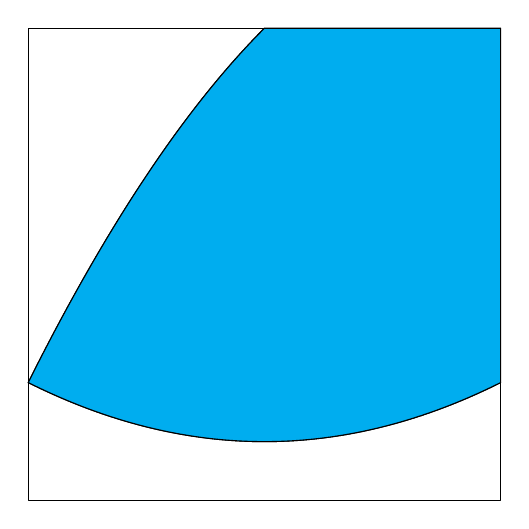
\begin{tikzpicture}[scale=0.6,>=stealth, font=\footnotesize, line join=round, line cap=round]
\draw (0,0)--(10,0)--(10,10)--(0,10)--cycle;
\draw plot[smooth,samples=100,domain=0:5] (\x,{-0.1*(\x)^2+2*(\x)+2.5}) ;
\draw plot[smooth,samples=100,domain=0:10] (\x,{0.05*(\x)^2-0.5*(\x)+2.5}) ;
\draw[fill=cyan] plot[smooth,samples=100,domain=0:10](\x,{0.05*(\x)^2-0.5*(\x)+2.5})--(10,10)--(5,10)--plot[smooth,samples=100,domain=5:0] (\x,{-0.1*(\x)^2+2*(\x)+2.5}) ;
\end{tikzpicture}
}
\shortans[oly]{$81$}
\loigiai{
\begin{center}
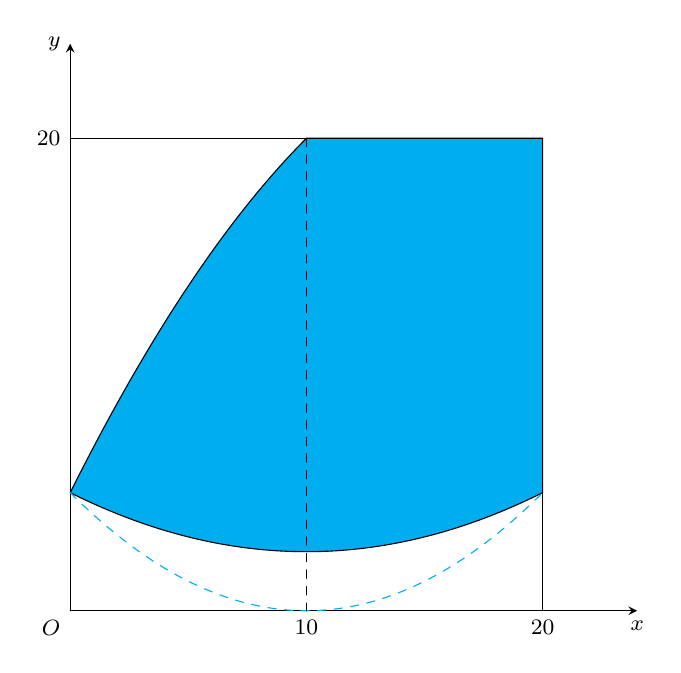
\begin{tikzpicture}[scale=0.6,>=stealth, font=\footnotesize, line join=round, line cap=round]
\draw [->] (0,0)--(12,0) node[below]{$x$} ;
\draw [->] (0,0)--(0,12) node[left]{$y$} ;
\draw[fill=cyan] plot[smooth,samples=100,domain=0:10](\x,{0.05*(\x)^2-0.5*(\x)+2.5})--(10,10)--(5,10)--plot[smooth,samples=100,domain=5:0] (\x,{-0.1*(\x)^2+2*(\x)+2.5}) ;
\draw (0,0)--(10,0)--(10,10)--(0,10)--cycle;
\draw[dashed,cyan] plot[smooth,samples=100,domain=0:10] (\x,{(\x)^2/10-\x+2.5)}) ;
%\draw plot[smooth,samples=100,domain=0:10] (\x,{0.05*(\x)^2-0.5*(\x)+2.5}) ;
\draw(0,0) node[below left]{$O$} (0,10) node[left]{$20$}  (10,0) node[below]{$20$} (5,0) node[below]{$10$};
\draw[dashed] (5,10)--(5,0) ;
\end{tikzpicture}
\end{center}
Diện tích hồ bơi chưa mở rộng là
\begin{align*}
S &= \int\limits_0^{10} \left ( -\dfrac{1}{20} x^2+2x+5 - \dfrac{1}{40} x^2+\dfrac{1}{2} x-5\right ) \mathrm{\,d}x + \int\limits_{10}^{20} \left ( 10 - \dfrac{1}{40} x^2+\dfrac{1}{2} x-5\right ) \mathrm{\,d}x  \\
& =\int\limits_0^{10} \left ( -\dfrac{3}{40} x^2+\dfrac{5}{2}x \right ) \mathrm{\,d}x + \int\limits_{10}^{20} \left ( -\dfrac{1}{40} x^2+\dfrac{1}{2} x+5\right ) \mathrm{\,d}x  \\
&= \dfrac{500}{3}.
\end{align*}
Parabol $(P) : y=ax^2+bx+c$ tiếp xúc với trục hoành tại $x=10$ suy ra
\[
\heva{&-\dfrac{b}{2a} =10\\&100a+10b+c =0} \Leftrightarrow \heva{&b=-20a\\&c=100a.}
\]
Suy ra $(P) : y= a(x^2-20x+100)$. \\
Diện tích hồ bơi khi mở rộng là
\begin{align*}
S'  &= \int\limits_0^{10} \left ( -\dfrac{1}{20} x^2+2x+5 - a(x^2-20x+100)\right ) \mathrm{\,d}x + \int\limits_{10}^{20} \left ( 10 - a(x^2-20x+100)\right ) \mathrm{\,d}x  \\
& =\int\limits_{0}^{10} \left (  -\dfrac{1}{20} x^2+2x+5 \right ) \mathrm{\,d}x
- a\int\limits_0^{10} \left ( x^2-20x+100 \right ) \mathrm{\,d}x + \int\limits_{10}^{20} 10 \mathrm{\,d}x
- a\int\limits_{10}^{20}(x^2-20x+100)\mathrm{\,d}x  \\
&= \dfrac{400}{3} - \dfrac{1000a}{3} + 100 - \dfrac{1000a}{3} \\
&= \frac{700-2000 a}{3}.
\end{align*}
Hồ mở rộng $20\%$ diện tích nên
\begin{align*}
& S' = 1{,}2S \\
\Leftrightarrow~& \frac{700-2000 a}{3}= 1{,}2 \cdot \dfrac{500}{3} \\
\Leftrightarrow~& a= \dfrac{1}{20}.
\end{align*}
Suy ra $b=-1$, $c=5$ (thỏa mãn). \\
Vậy $T= 20(a+b+c) =81$.
}
\end{ex}

\begin{ex}%[Đề kiểm tra giữa kì 2 - THPT Thanh Miện, Hải Dương, Nguyễn Anh Tuấn, Dự án 12EX-3-2026]%[2D4C3-2]
Cho một mảnh vườn hình chữ nhật $ABCD$ có chiều rộng là $2$ m, chiều dài gấp ba chiều rộng. Người ta chia mảnh vườn bằng cách dùng hai đường parabol, mỗi đường parabol có đỉnh là trung điểm mỗi cạnh dài và đi qua hai mút của canh dài đối diện. Tính tỉ số diện tích phần mảnh vườn nằm ở miền trong hai parabol với diện tích phần còn lại. (kết quả làm tròn đến hàng phần trăm)
\shortans[oly]{0,89}
\begin{center}
\begin{tikzpicture}[>=stealth, scale=1]
% 1. Vẽ trục tọa độ
\draw[->] (-4,0) -- (4,0) node[above] {$x$};
\draw[->] (0,-0.5) -- (0,3) node[right] {$y$};

% 2. Vẽ hình chữ nhật ABCD (Nằm trên trục hoành, cao 2m, dài 6m)
\draw (-3,0) rectangle (3,2);

% 3. Vẽ miền gạch chéo (Phần giao giữa 2 Parabol)
% Giao điểm tại x = +-sqrt(4.5) approx +-2.121
\begin{scope}
\clip (-3,0) rectangle (3,2);
\fill[pattern=north west lines, pattern color=gray!70]
plot[domain=-2.121:2.121, samples=300] (\x, {(2/9)*(\x)^2}) --
plot[domain=2.121:-2.121, samples=300] (\x, {-(2/9)*(\x)^2 + 2}) -- cycle;
\end{scope}

% 4. Vẽ 2 đường Parabol
% Parabol ngửa: y = (2/9)x^2
\draw[blue, domain=-3.5:3.5, samples=300] plot (\x, {(2/9)*(\x)^2});
% Parabol úp: y = -(2/9)x^2 + 2
\draw[red, domain=-3.5:3.5, samples=300] plot (\x, {-(2/9)*(\x)^2 + 2});


\foreach \x/\y in{-3/0,3/0,3/2,-3/2,0/0,0/2}\draw[fill=black](\x,\y)circle(1.25pt);
\foreach \x/\y/\goc/\z in{-3/0/-70/D,3/0/-120/C,-3/2/-180/A,3/2/15/B,0/0/-130/O}
\path(\x,\y)node[shift={(\goc:7pt)}]{\scriptsize$\z$};
\end{tikzpicture}
\end{center}
\loigiai{
\begin{center}
\begin{tikzpicture}[>=stealth, scale=1]
% 1. Vẽ trục tọa độ
\draw[->] (-4,0) -- (4,0) node[above] {$x$};
\draw[->] (0,-0.5) -- (0,3) node[right] {$y$};

% 2. Vẽ hình chữ nhật ABCD (Nằm trên trục hoành, cao 2m, dài 6m)
\draw (-3,0) rectangle (3,2);

% 3. Vẽ miền gạch chéo (Phần giao giữa 2 Parabol)
% Giao điểm tại x = +-sqrt(4.5) approx +-2.121
\begin{scope}
\clip (-3,0) rectangle (3,2);
\fill[pattern=north west lines, pattern color=gray!70]
plot[domain=-2.121:2.121, samples=300] (\x, {(2/9)*(\x)^2}) --
plot[domain=2.121:-2.121, samples=300] (\x, {-(2/9)*(\x)^2 + 2}) -- cycle;
\end{scope}

% 4. Vẽ 2 đường Parabol
% Parabol ngửa: y = (2/9)x^2
\draw[blue, domain=-3.5:3.5, samples=300] plot (\x, {(2/9)*(\x)^2});
% Parabol úp: y = -(2/9)x^2 + 2
\draw[red, domain=-3.5:3.5, samples=300] plot (\x, {-(2/9)*(\x)^2 + 2});


\foreach \x/\y in{-3/0,3/0,3/2,-3/2,0/0,0/2}\draw[fill=black](\x,\y)circle(1.25pt);
\foreach \x/\y/\goc/\z in{-3/0/-70/D,3/0/-120/C,-3/2/-180/A,3/2/15/B,0/0/-130/O}
\path(\x,\y)node[shift={(\goc:7pt)}]{\scriptsize$\z$};
\end{tikzpicture}
\end{center}
Chọn hệ trục tọa độ $Oxy$ như hình vẽ, với gốc tọa độ $O$ là trung điểm của cạnh $CD$.\\
Khi đó $A(-3;2)$, $B(3;2)$, $C(3;0)$, $D(-3;0)$.
\begin{itemize}
\item Parabol thứ nhất $(P_1)$ có đỉnh là $O(0;0)$ và đi qua hai điểm $A(-3;2)$, $B(3;2)$ nên có phương trình dạng $y=ax^2$.\\
Thay tọa độ điểm $B$ vào, ta được: $2 = a \cdot 3^2 \Rightarrow a = \dfrac{2}{9}$.\\
Vậy $(P_1) \colon y = \dfrac{2}{9}x^2$.
\item Parabol thứ hai $(P_2)$ có đỉnh là trung điểm cạnh $AB$ tức $(0;2)$ và đi qua hai điểm $C(3;0)$, $ D(-3;0)$ nên có phương trình dạng $y=ax^2+b$.\\
Vì đỉnh tại $(0;2)$ nên $b=2$. \\
Thay tọa độ $C(3;0)$, ta có $0 = a \cdot 3^2 + 2 \Rightarrow a = -\dfrac{2}{9}$.\\
Vậy $(P_2)\colon y = -\dfrac{2}{9}x^2 + 2$.
\end{itemize}
Phương trình hoành độ giao điểm của $(P_1)$ và $(P_2)$ là
\[ \dfrac{2}{9}x^2=-\dfrac{2}{9}x^2 + 2 \Leftrightarrow \dfrac{4}{9}x^2=2\Leftrightarrow x^2 = \dfrac{9}{2} \Leftrightarrow x = \pm \dfrac{3\sqrt{2}}{2}.\]
Diện tích phần mảnh vườn nằm ở miền trong hai parabol là
\[ S_1 = \displaystyle\int\limits_{-\frac{3\sqrt{2}}{2}}^{\frac{3\sqrt{2}}{2}} \left| \left(-\dfrac{2}{9}x^2 + 2\right) - \dfrac{2}{9}x^2 \right| \mathrm{\,d}x = \displaystyle\int\limits_{-\frac{3\sqrt{2}}{2}}^{\frac{3\sqrt{2}}{2}} \left( 2 - \dfrac{4}{9}x^2 \right) \mathrm{\,d}x.\]
Diện tích hình chữ nhật $ABCD$ là $S_{ABCD} = 6 \cdot 2 = 12$ (m$^2$).\\
Diện tích phần còn lại của mảnh vườn là $S_2 = S_{ABCD} - S_1 = 12 - 4\sqrt{2}$ (m$^2$).\\
Tỉ số diện tích cần tìm là $ T = \dfrac{S_1}{S_2}=\dfrac{4\sqrt{2}}{12 - 4\sqrt{2}} \approx 0{,}89$.\\
Vậy tỉ số diện tích là $0{,}89$.
}
\end{ex}

\begin{ex}%[Dự án TN THPT 2026]%[Thầy Nguyễn Đức Tuấn Anh]%[2D4C3-2]
\immini[thm]{Bạn An thực hiện thiết kế một logo hình con mắt cho một phòng khám nhãn khoa. Logo là một hình phẳng giới hạn bởi hai parabol $y=f(x)$ và $y=g(x)$ có các kích thước như hình vẽ dưới đây (phần được tô màu đen) và một hình tròn có bán kính bằng $0{,}5$ dm ở giữa là phần con ngươi (phần được tô màu xanh), đơn vị trên mỗi trục tọa độ là decimet. Biết rằng chi phí để sơn phần con ngươi hình tròn màu xanh là $25\,000$ đồng/dm$^2$ và chi phí để sơn phần còn lại màu đen là $20\,000$ đồng/dm$^2$. Chi phí để sơn logo trên là bao nhiêu nghìn đồng (\textit{làm tròn kết quả đến hàng đơn vị})?}{
\begin{tikzpicture}[scale=1, font=\footnotesize, line join=round, line cap=round, >=stealth]
\fill[gray!50!white, domain=-2.45:2.45] plot (\x,{-(\x)^2/4+2})-- plot (\x,{(\x)^2/4-1})--cycle;
\draw[fill=cyan!50!white] (0,0.5) circle (0.5cm);
\draw[->] (-2.5,0)--(2.5,0) node[above] {$x$};
\draw[->] (0,-1.5)--(0,2.5) node[right] {$y$};
\foreach \x/\y/\z/\t in {-2/-2/0/-135,O/0/0/-135,2/2/0/-90,-1/0/-1/-135,1/0/1/135,2/0/2/135,/0/0.5/0} {\draw (\y,\z) circle (1pt) ($(\y,\z)+(\t:3mm)$) node {$\x$};}
\draw[dashed] (-2,0)--(-2,1)--(2,1)--(2,0);
\draw[domain=-2.45:2.45,samples=100] plot (\x,{-(\x)^2/4+2});
\draw[domain=-2.45:2.45,samples=100] plot (\x,{(\x)^2/4-1});
\foreach \x in {-2.45,2.45} {\draw[fill=black] (\x,{(\x)^2/4-1}) circle (1pt);}
\end{tikzpicture}
}
\par
\shortans[0]{200}
\loigiai{
Gọi phương trình parabol $y=f(x)$ là $f(x)=ax^2+bx+c$ với $a\neq 0$ đi qua các điểm có toạ độ lần lượt là $(2;1)$, $(0;2)$, $(-2;1)$.\\
Lập hệ phương trình ba ẩn, từ đó suy ra được $\heva{&a=-\dfrac{1}{4}\\&b=0\\&c=2}$ nên $f(x)=-\dfrac{1}{4}x^2+2$.\\
Gọi phương trình parabol $y=g(x)$ là $g(x)=mx^2+nx+p$ với $m\neq 0$ đi qua các điểm có toạ độ lần lượt là $(-2;0)$, $(0;-1)$, $(2;0)$.\\
Lập hệ phương trình ba ẩn, từ đó suy ra được $\heva{&m=\dfrac{1}{4}\\&n=0\\&p=-1}$ nên $g(x)=\dfrac{1}{4}x^2-1$.\\
Phương trình hoành độ giao điểm $f(x)=g(x)\Leftrightarrow -\dfrac{1}{4}x^2+2=\dfrac{1}{4}x^2-1\Leftrightarrow \dfrac{1}{2}x^2=3\Leftrightarrow x=\pm \sqrt{6}$.\\
Diện tích hình tròn được sơn màu xanh là $S_1=\pi r^2=\pi (0{,}5)^2=0{,}25\pi $ (dm$^2$).\\
Diện tích hình phẳng được giới hạn bởi $y=f(x)$ và $y=g(x)$ là
\[S_2=\displaystyle \int \limits _{-\sqrt{6}}^{\sqrt{6}}\left|f(x)-g(x) \right|\mathrm{d}x=\displaystyle \int \limits _{-\sqrt{6}}^{\sqrt{6}}\left|\left(-\dfrac{1}{4}x^2+2\right) -\left(\dfrac{1}{4}x^2-1\right) \right|\mathrm{d}x.\]
Diện tích phần sơn được tô màu đen là \[S_3=S_2-S_1=\displaystyle \int \limits _{-\sqrt{6}}^{\sqrt{6}}\left|\left(-\dfrac{1}{4}x^2+2\right) -\left(\dfrac{1}{4}x^2-1\right) \right|\mathrm{d}x=0{,}25\pi. \]
Chi phí để sơn logo là\\
$T=0{,}25\pi \cdot 25\,000+\left(\displaystyle \int \limits _{-\sqrt{6}}^{\sqrt{6}}\left|\left(-\dfrac{1}{4}x^2+2\right) -\left(\dfrac{1}{4}x^2-1\right) \right|\mathrm{d}x-0{,}25\pi \right)\cdot 20\,000=200$ (nghìn đồng).
}
\end{ex}

\begin{ex}%[2D4C3-2]
\immini{
Một bức tường hình chữ nhật $ABCD$ có kích thước $6$ m $\times 4$ m được bạn An trang trí bằng cách vẽ hai đồ thị $f(x)=a^x$, $g(x)=\log _bx$ đối xứng nhau qua đường thẳng $d\colon y=x$ và chia thành ba phần \textit{(tham khảo hình vẽ bên)}.
Phần $H_1$ được sơn màu xanh da trời, phần $H_2$ được sơn màu vàng, phần $H_3$ được sơn màu xanh lá cây. Biết rằng mỗi hộp sơn các màu chỉ sơn được $3$ m$^2$ tường, đồng thời giá của hộp sơn màu xanh da trời là $100\,000$ đồng/hộp, hộp sơn vàng là $140\,000$ đồng/hộp, hộp sơn xanh lá cây là $130\,000$ đồng/hộp. Tính giá tiền bạn Hà mua để sơn bức tường này? \textit{(đơn vị là triệu đồng và cửa hàng sơn chỉ bán số nguyên của hộp)}.
}{
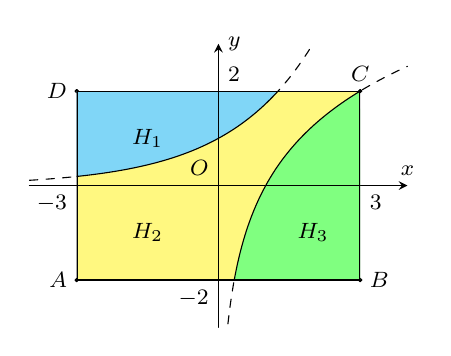
\begin{tikzpicture}[scale=0.6,font=\footnotesize,line join=round,line cap=round,>=stealth]
\draw[->] (-4,0)--(4,0) node[above] {$x$};
\draw[->] (0,-3)--(0,3) node[right] {$y$};
\draw[dashed,domain=-4:2,samples=100] plot(\x,{(3)^(0.5*\x)});
\draw[dashed,domain=0.2:4,samples=100] plot(\x,{2*ln(\x)/ln(3)});
\coordinate (A) at (-3,-2);
\coordinate (B) at (3,-2);
\coordinate (C) at (3,2);
\coordinate (D) at (-3,2);
\foreach \x in {A,B,C,D} {\draw[fill=black] (\x) circle(1pt);}
\node[left] at (A) {$A$};
\node[left] at (D) {$D$};
\node[right] at (B) {$B$};
\node[above] at (C) {$C$};
\node[above right] at (0,2) {$2$};
\node[below left] at (-3,0) {$-3$};
\node[below right] at (3,0) {$3$};
\node[below left] at (0,-2) {$-2$};
\clip (-3,2) rectangle (3,-2);
\fill[yellow!50!white] (-3,2) rectangle (3,-2);
\fill[cyan!50!white] (-3,2) -- plot(\x,{(3)^(0.5*\x)})--cycle;
\fill[green!50!white] plot[domain=0.2:3](\x,{2*ln(\x)/ln(3)})--(3,-2)--cycle;
\draw[domain=-4:2,samples=100] plot(\x,{(3)^(0.5*\x)});
\draw[domain=0.2:4,samples=100] plot(\x,{2*ln(\x)/ln(3)});
\draw[->] (-4,0)--(4,0) node[above] {$x$};
\draw[->] (0,-3)--(0,3) node[right] {$y$};
\draw[thick] (A)--(B)--(C)--(D)--cycle;
\node at (-1.5,1) {$H_1$};
\node at (-1.5,-1) {$H_2$};
\node at (2,-1) {$H_3$};
\node[above left] at (0,0) {$O$};
\end{tikzpicture}
}
\par
\shortans[0]{1{,}15}
\loigiai{
Hai đồ thị $f(x)=a^x$, $g(x)=\log _bx$ đối xứng nhau qua đường thẳng $(d)\colon y=x$ khi $a=b$.\\
Điểm $(3;2)$ thuộc đồ thị hàm số $g(x)=\log _bx$ nên $\log _b3=2\Leftrightarrow b^2=3 \Rightarrow a=b=\sqrt{3}$.\\
Ta có $S_{H_1}+S_{H_2}+S_{H_3}=S_{ABCD}=6\cdot 4=24$ m$^2$.\\
Xét $\left(\sqrt{3}\right)^x=2\Leftrightarrow x=\log _{\sqrt{3}}2\Rightarrow S_{H_1}=\displaystyle \int \limits_{-3}^{\log _{\sqrt{3}}2}\left(2-\left(\sqrt{3}\right)^x\right)\mathrm{\,d}x\approx 5{,}23$ m$^2$ nên cần mua $2$ hộp sơn màu xanh da trời.\\
Xét $\log _{\sqrt{3}}x=-2\Leftrightarrow x=\dfrac{1}{3}\Rightarrow S_{H_3}=\displaystyle \int \limits_{\frac{1}{3}}^3\left(\log _{\sqrt{3}}x+2\right)\mathrm{\,d}x\approx 7{,}14$ m$^2$ nên cần mua $3$ hộp sơn màu xanh lá cây.\\
Ta có $\dfrac{S_{H_2}}{3}=\dfrac{24-S_{H_1}-S_{H_3}}{3}\approx 3{,}87\Rightarrow S_{H_2}\approx 11{,}61$ m$^2$ nên cần mua $4$ hộp sơn màu vàng.\\
Số tiền mua sơn là $2\cdot 0{,}1+3\cdot 0{,}13+4\cdot 0{,}14=1{,}15$ (triệu đồng).
}
\end{ex}

\begin{ex}%[2D4C3-3]
\immini{
Một vật trang trí có dạng một khối tròn xoay được tạo thành khi xoay miền $(R)$ (phần gạch chéo trong hình vẽ bên) quanh trục $AB$. Miền $(R)$ được giới hạn bởi các cạnh $AB$, $AD$ của hình vuông $ABCD$ và các cung phần tư của các đường tròn bán kính bằng $1$ cm với tâm lần lượt là trung điểm của các cạnh $BC$, $AD$. Tính thể tích của vật trang trí đó (đơn vị cm$^3$), làm tròn kết quả đến hàng phần mười.
}{
\begin{tikzpicture}
\coordinate (A) at (0,0);
\coordinate (B) at (0,-4);
\coordinate (C) at (4,-4);
\coordinate (D) at (4,0);
\draw (A)--(B)--(C)--(D)--(A);
\draw[pattern=north east lines] (B) arc (180:90:2) arc (-90:0:2)--(A)--(B);
\path node at (A) [above left]{$A$}
node at (B) [below left] {$B$}
node at (C) [below right] {$C$}
node at (D) [above right] {$D$};
\end{tikzpicture}
}
\shortans{$10{,}5$}
\loigiai{
\begin{center}
\begin{tikzpicture}
\draw [->] (0,-4) --(5,-4);
\draw [->] (0,-4) --(0,1);
\coordinate (D) at (0,0);
\coordinate (A) at (0,-4);
\coordinate (B) at (4,-4);
\coordinate (C) at (4,0);
\coordinate (I) at (4,-2);
\coordinate (J) at (0,-2);
\coordinate (K) at (2,-2);
\draw (A)--(B)--(C)--(D)--(A);
\draw[pattern=north west lines,opacity=0.4] (D) arc (90:0:2) arc (180:270:2)--(B)--(A)--(D);
\foreach \x in {A,B,C,D,I,J,K}{
\fill (\x) circle (1pt);
}

\draw[line width=1.5pt, red] (D) arc (90:0:2);
\draw[dashed, opacity=0.4,red] (D) arc (90:450:2);
\draw[line width=1.5pt, blue] (K) arc (180:270:2);
\draw[dashed, opacity=0.4,blue] (K) arc (180:540:2);

\path node at (D) [above left]{$D$}
node at (A) [below left] {$A\equiv O$}
node at (B) [below right] {$B$}
node at (C) [above right] {$C$}
node at (I) [left] {$I$}
node at (J) [left] {$J$}
node at (5,-4) [below] {$x$}
node at (0,1) [left] {$y$}
node at (K) [right] {$K$}
node at (2.6,-0.3) {$y=1+\sqrt{1-x^2}$}
node at (4.2,-3) {$y=1-\sqrt{1-(x-2)^2}$};
\end{tikzpicture}
\end{center}
Ta xoay hình lại và đưa vào hệ trục tọa độ như trên hình vẽ. Khi đó phần gạch chéo trên hình sẽ quay quanh trục $Ox$.\\
Đường tròn tâm $J$
\allowdisplaybreaks
\begin{eqnarray*}
x^2+(y-1)^2=1&\Rightarrow& (y-1)^2=1-x^2\\
& \Leftrightarrow& |y-1|=\sqrt{1-x^2}\\
& \Leftrightarrow &\heva{& y-1 =\sqrt{1-x^2}, \mbox{ khi } y\ge 1 \\& -(y-1) =\sqrt{1-x^2}, \mbox{ khi } y< 1} \\
&\Leftrightarrow& \heva{& y =1+\sqrt{1-x^2}, \mbox{ khi } y\ge 1 \\& y=1-\sqrt{1-x^2} , \mbox{ khi } y< 1.}
\end{eqnarray*}
Suy ra đồ thị đường cong từ $D$ đến $K$ là $y=1+\sqrt{1-x^2}$ với $x\in [0;1]$.\\
Đường tròn tâm $I$
\begin{eqnarray*}
(x-2)^2+(y-1)^2=17&\Rightarrow& (y-1)^2=1-(x-2)^2 \\
&\Leftrightarrow& |y-1|=\sqrt{1-(x-2)^2}\\
&\Leftrightarrow& \heva{& y-1 =\sqrt{1-(x-2)^2}, \mbox{ khi } y\ge 1 \\& -(y-1) =\sqrt{1-(x-2)^2}, \mbox{ khi } y< 1}\\
&\Leftrightarrow& \heva{& y =1+\sqrt{1-(x-2)^2}, \mbox{ khi } y\ge 1 \\& y=1-\sqrt{1-(x-2)^2} , \mbox{ khi } y< 1}
\end{eqnarray*}
Suy ra đồ thị đường cong từ $K$ đến $B$ là $y=1-\sqrt{1-(x-2)^2}$ với $x\in [1;2]$.\\
Đường cong đi từ $D$ đến $B$ trên hình gồm hai phần$\colon$ phần thứ nhất là một phần tư đường tròn đi từ $D$ đến $K$ của đường tròn tâm $J$ và phần thứ hai là một phần tư đường tròn đi từ $K$ đến $B$ của đường tròn tâm $I$.\\
Thể tích của vật trang trí là
\[V= \pi\displaystyle\int\limits_0^1 \left(1+\sqrt{1-x^2}\right)^2\mathrm{\,d}x +  \pi\displaystyle\int\limits_1^2 \left(1-\sqrt{1-(x-2)^2}\right)^2\mathrm{\,d}x \approx 10{,}5 \mbox{ cm}^3.\]
}
\end{ex}

\begin{ex}%[2D4C3-3]Biên soạn:Phùng Hoàng Em Phản biện:Nguyễn Đắc Kiên
\immini[thm]
{Gọi $(\mathscr{H})$ là hình phẳng giới hạn bởi đồ thị $(\mathscr{C})$ của hàm số $y=\sqrt{x}$, trục $Ox$ và đường thẳng $x=9$. Cho điểm $M$ thuộc đồ thị $(\mathscr{C})$ và điểm $A(9;0)$. Gọi $V_1$ là thể tích khối tròn xoay tạo thành khi hình phẳng $(\mathscr{H})$ quay quanh trục $Ox$, $V_2$ là thể tích khối tròn xoay tạo thành khi tam giác $OMA$ quay quanh trục $Ox$.}
{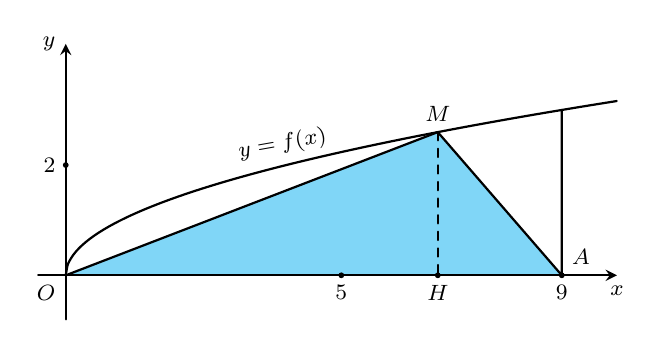
\begin{tikzpicture}[>=stealth,scale=0.7, line join=round, line cap=round,thick,font=\footnotesize]
\def\xt{-0.5} \def\xp{10} \def\yt{4.2} \def\yd{-0.8}
\fill[cyan!50!white](0,0)--(6.75,2.598)--(9,0)--cycle;
\draw[->] (\xt,0)--(\xp,0) node [below]{$x$};
\draw[->] (0,\yd)--(0,\yt) node [left]{$y$};
\node at (0,0) [below left]{$O$};
\node at (4,2) [above,rotate=10] {$y=f(x)$};
\fill (0,2)node [left]{$2$} circle(1.5pt);
\foreach \x in {5,9} \fill (\x,0)node[below]{$\x$} circle(1.5pt);
\draw[smooth,samples=300,domain=0:10] plot(\x,{sqrt(\x)});
\draw (0,0)--(6.75,2.598)--(9,0)--(9,3);
\draw[dashed](6.75,2.598)--(6.75,0);
\fill (6.75,2.598)node[above]{$M$} (9,3) (6.75,0)node[below]{$H$} circle(1.5pt);
\node at (9,0)[above right]{$A$};
\end{tikzpicture}}
\vspace{0.3cm}
\noindent
Biết rằng $V_1=2V_2$. Tính diện tích $S$ phần hình phẳng giới hạn bởi đồ thị $(\mathscr{C})$ và đường thẳng $OM$ (\textit{làm tròn đến hàng phần trăm}).
\shortans{$2{,}92$}
\loigiai
{Theo bài ra ta có $V_1=\pi\displaystyle\int\limits_{0}^{9}(\sqrt{x})^2\mathrm{\,d}x=\dfrac{81\pi}{2}$.\\
Gọi $H$ là hình chiếu vuông góc của $M$ trên trục $Ox$.\\
Đặt $OH=m$ (với $0<m<9$), khi đó $M(m;\sqrt{m})$, $MH=\sqrt{m}$, $AH=9-m$.\\
Suy ra
\[V_2=\dfrac{1}{3}\pi\cdot MH^2\cdot OH + \dfrac{1}{3}\pi\cdot MH^2\cdot AH = \dfrac{1}{3}\pi\cdot MH^2\cdot OA = 3m\pi.\]
Theo giả thiết $V_1=2V_2$ nên $\dfrac{81\pi}{2}=6m\pi \Leftrightarrow m=\dfrac{27}{4}$. Do đó $M\left(\dfrac{27}{4};\dfrac{3\sqrt{3}}{2}\right)$.\\
Phương trình đường thẳng $OM$ là $y=\dfrac{2\sqrt{3}}{9}x$.\\
Vậy diện tích hình phẳng giới hạn bởi đồ thị $(C)$ và đường thẳng $OM$ là
\[S=\displaystyle\int\limits_{0}^{\tfrac{27}{4}} \left(\sqrt{x} - \dfrac{2\sqrt{3}}{9}x\right)\mathrm{\,d}x = \left(\dfrac{2}{3}x\sqrt{x}-\dfrac{\sqrt{3}}{9}x^2\right)\Bigg|_{0}^{\tfrac{27}{4}} = \dfrac{27\sqrt{3}}{16} \approx 2{,}92.\]
}
\end{ex}

\begin{ex}%[2D4C3-3]
\immini{
Cho nửa lục giác đều $ABCD$ nội tiếp đường tròn đường kính $AD=8$ (tham khảo hình vẽ). Thể tích khối tròn xoay được tạo thành khi quay miền tứ giác $ABCD$ quanh đường thẳng $CD$ bằng $a\pi$. Tìm $a$.
}
{\begin{tikzpicture}[font=\footnotesize,line join=round, line cap=round, >=stealth,scale=0.55]
\def\r{4}
\path ($(0,0)$) coordinate (O);
\foreach \x/\pos in {180/A, 120/B, 60/C, 0/D} \path ($(O)+(\x:\r)$) coordinate (\pos);
\fill[pattern=north west lines,opacity=.6] (A)--(B)--(C)--(D)--(A);
\draw (A)--(B)--(C)--(D)--(A) (O) circle (\r) ;
\fill (0,0) circle(1pt);
\foreach \x/\pos in {A/180, B/120, C/60, D/0} \fill (\x) circle(1pt) node[{shift=(\pos:0.25)}]{$\x$};
\end{tikzpicture}}
\shortans{$112$}
\loigiai{
\begin{center}
\begin{tikzpicture}[font=\footnotesize,line join=round, line cap=round, >=stealth,scale=0.75]
\def\r{4}
\def \xmin{-1}\def \xmax{7}\def \ymin{-1}\def \ymax{8}
\draw[->] (\xmin,0)--(\xmax,0) node[shift=(-90:0.25)] {$x$};
\draw[->] (0,\ymin)--(0,\ymax) node[shift=(0:0.25)] {$y$};
\fill (0,0) circle(1pt) node[shift=(-135:0.25)]{$O$}
(4,0) circle(1pt) node[shift=(-45:0.2)]{$4$}
(6,0) circle(1pt) node[shift=(-90:0.2)]{$6$}
(0,{4*sqrt(3)}) circle(1pt) node[left]{$4\sqrt{3}$}
(0,{2*sqrt(3)}) circle(1pt) node[left]{$2\sqrt{3}$};
\path ($(0,0)$) coordinate (D)
($(\r,0)$) coordinate (C)
($(D)+(60:2*\r)$) coordinate (A)
($(C)+(60:\r)$) coordinate (B);
\fill[pattern=north west lines,opacity=.6] (A)--(B)--(C)--(D)--(A);
\draw[dashed] (A)--(C) (0,{2*sqrt(3)})--(B)--(6,0) (0,{4*sqrt(3)})--(A);
\draw (D)--(A)--(B)--(C);
\foreach \x/\pos in {A/90, B/0, C/-135, D/135} \fill (\x) circle(1pt) node[{shift=(\pos:0.25)}]{$\x$};
\end{tikzpicture}
\end{center}
Đặt hệ trục tọa độ $Oxy$ như hình vẽ. Khi đó, ta có $A(4;4\sqrt{3})$, $B(6;2\sqrt{3})$, $C(4;0)$ và $D(0;0)$.\\
Phương trình đường thẳng $AD$ là $y=\sqrt{3}x$.\\
Phương trình đường thẳng $AB$ là $y=-\sqrt{3}x+8\sqrt{3}$.\\
Phương trình đường thẳng $BC$ là $y=\sqrt{3}x-4\sqrt{3}$.\\
Suy ra thể tích khối tròn xoay được tạo thành khi quay miền tứ giác $ABCD$ quanh đường thẳng $CD$ là
\begin{align*}
\displaystyle V&=\pi\int\limits_{0}^{4}\left(\sqrt{3}x\right)^2 \mathrm{\, d} x+ \pi\int\limits_{4}^{6}\left(\left(-\sqrt{3}x+8\sqrt{3}\right)^2-\left(\sqrt{3}x-4\sqrt{3}\right)^2\right)\mathrm{\, d} x\\
&=\pi\int\limits_{0}^{4}3x^2 \mathrm{\, d} x+ 3\pi\int\limits_{4}^{6}\big(-8x+48\big)\mathrm{\, d} x\\
&=\pi \cdot x^3\Big|_{0}^{4}+3\pi\big(-4x^2+48x\big)\Big|_{4}^{6}\\
&=64\pi+48\pi=112\pi.
\end{align*}
}
\end{ex}

\begin{ex}%[2D4C3-3]
Cho hàm số $ y=f(x)=a{x^3}+b{x^2}+cx+d,\left(a,b,c,d\in\mathbb{R},a\ne 0\right)$ có đồ thị $(C)$. Biết rằng đồ thị $(C)$ tiếp xúc với đường thẳng $ y=4$ tại điểm có hoành độ âm và đồ thị của hàm số $ y=f'(x)$ cho bởi hình vẽ dưới đây. Tính thể tích vật thể tròn xoay được tạo thành khi quay hình phẳng $ H$ giới hạn bởi đồ thị $(C)$ và trục hoành khi quay xung quanh trục $Ox$. (kết quả làm tròn đến hàng phần mười)
\shortans{$65{,}4$}
\begin{center}
\begin{tikzpicture}[line cap=butt,line join=miter,>=stealth]
\tikzset{declare function={xmin=-2;xmax=2;ymin=-4;ymax=2;
f(\x)=3*(\x)^2-3;
},
smooth,samples=450
}
\draw[->] (xmin,0)--(xmax,0) node[shift={(-100:7pt)},font=\normalsize]{$ x $};
\draw[->] (0,ymin)--(0,ymax) node[shift={(190:7pt)},font=\normalsize]{$ y $};
\fill (0,0) node[shift={(-135:11pt)},font=\normalsize]{$ O $};
\draw (-1,0)node[below left]{$-1$} circle (1pt)
(1,0)node[below right]{$1$} circle (1pt)
(0,-3)node[below left]{$-3$} circle (1pt);
\draw  plot[domain=-1.28:1.28] (\x, {f(\x)})node[above left,font=\footnotesize,rotate=80]{$y=f'(x)$};
\end{tikzpicture}
\end{center}
\loigiai{
Phương trình $f'(x)=0$ có hai nghiệm phân biệt là $-1;1$\\
$\Rightarrow{f}'(x)=k\left(x+1\right)\left(x-1\right)$.\\
Mà $f'(0)=-3\Leftrightarrow k\cdot 1\cdot \left(-1\right)=-3\Leftrightarrow k=3$.\\
Do đó: $f'(x)=3\left(x+1\right)\left(x-1\right)\Rightarrow{f}'(x)=3x^2-3$.\\
$\Rightarrow f(x)=\displaystyle\int{f'(x)\mathrm{d}x}=\displaystyle\int{\left(3x^2-3\right)\mathrm{d}x}=x^3-3x+C$.\\
Đồ thị $(C)$ của hàm số $ y=f(x)$ tiếp xúc với đường thẳng $ y=4$ tại điểm có hoành độ âm, nghĩa là đường thẳng $(d):y=4$ là tiếp tuyến của đồ thị $(C)$ tại điểm có hoành độ $x_0$ âm.\\
$\Rightarrow{f}'\left(x_0\right)=k_d\Leftrightarrow 3x_0^2-3=0\Leftrightarrow\hoac{&{x_0}=1\\&{x_0}=-1.}$.\\
Vì $x_0$ âm, nên $x_0=-1$.\\
Ta có: $ f\left(x_0\right)=4\Leftrightarrow{\left(-1\right)^3}-3\left(-1\right)+C=4\Leftrightarrow C=2$.\\
Do đó: $ f(x)=x^3-3x+2$. Xét: $ f(x)=0\Leftrightarrow{x^3}-3x+2=0\Leftrightarrow\hoac{& x=1\\& x=-2.}$\\
Hình phẳng $(H)$ được giới hạn bởi: $\heva{& y=f(x);y=0\\& x=1;x=-2.}$\\
Thể tích vật thể tròn xoay được tạo thành khi quay hình phẳng $ H$ quanh trục $Ox$ là \begin{center}
$ V=\pi\displaystyle\int\limits_{-2}^1f^2(x)\mathrm{d}x=\dfrac{729}{35}\pi\approx65{,}4$.
\end{center}
}
\end{ex}

\begin{ex}%[2D4C3-4]
Có một cốc thủy tinh hình trụ, bán kính trong lòng đáy cốc là $4$ cm, chiều cao trong lòng cốc là $12$ cm đang đựng một lượng nước. Tính thể tích (đơn vị cm$^3$) lượng nước trong cốc , biết rằng khi nghiêng cốc nước vừa lúc nước chạm miệng cốc, mực nước trùng với đường kính đáy.
\begin{center}
\begin{tikzpicture}[line join=round,line cap=round,font=\footnotesize,scale=1,x=0.7cm]
\coordinate (A) at (1.5,0);
\coordinate (O) at (0,0);
\coordinate (A1) at ($(A)+(90:4)$);
\coordinate (O1) at ($(O)+(90:4)$);
\fill[cyan!20] (A) arc (0:-180:1.5 and 0.3)--++(0,1) arc (180:0:1.5 and 0.3)--cycle;
\draw (A) arc (0:-180:1.5 and 0.3)--($(A1)!2!(O1)$) arc (180:0:1.5 and 0.3) arc (0:-180:1.5 and 0.3) (A)--(A1);
\draw[dashed] (A) arc (0:180:1.5 and 0.3) ($(A)+(0,1)$) arc (0:180:1.5 and 0.3);
\draw ($(A)+(0,1)$) arc (0:-180:1.5 and 0.3);
\end{tikzpicture}
\quad\quad
\begin{tikzpicture}[line join=round,line cap=round,font=\footnotesize,scale=1,x=0.7cm]
\begin{scope}[rotate=-70]
\coordinate[] (A) at (1.5,0);
\coordinate[] (O) at (0,0);
\coordinate[] (A1) at ($(A)+(90:4)$);
\coordinate[] (O1) at ($(O)+(90:4)$);
\fill[cyan!20] ($(0,0)+(-70:1.5cm and 0.3cm)$)--($(0,0)+(110:1.5cm and 0.3cm)$)--($(A)+(90:4)$)--(A) arc (0:-70:1.5 and 0.3)--cycle;
\draw (A) arc (0:-180:1.5 and 0.3)--($(A1)!2!(O1)$) arc (180:0:1.5 and 0.3) arc (0:-180:1.5 and 0.3) (A)--(A1);
\draw[dashed] (A) arc (0:180:1.5 and 0.3);
\draw[dashed] ($(0,0)+(-70:1.5cm and 0.3cm)$)--($(0,0)+(110:1.5cm and 0.3cm)$)--($(A)+(90:4)$)--(0,0);
\draw ($(A)+(90:4)$)--($(0,0)+(-70:1.5cm and 0.3cm)$) ;
\end{scope}
\end{tikzpicture}
\end{center}
\shortans{$128$}
\loigiai{
\immini{
Chọn hệ trục tọa độ như hình vẽ.\\
Cắt khối nước trong cốc khi nằm nghiêng theo mặt phẳng vuông góc với trục $Ox$ ta được thiết diện là tam giác $ABC$ vuông tại $B$.\\
Ta có $AB=BC \cdot \tan \alpha =\sqrt{R^2-x^2} \cdot \tan \alpha$\\
Suy ra $ S_{\triangle ABC}=\dfrac{1}{2} \cdot AB \cdot BC=\dfrac{1}{2}(R^2-x^2) \cdot \tan\alpha =\dfrac{1}{2}(R^2-x^2) \cdot \dfrac{h}{R}$.\\
Do đó $ V=\dfrac{1}{2}\displaystyle\int\limits_{-4}^4 (R^2-x^2)\dfrac{h}{R}\mathrm{\,d}x=\dfrac{1}{2}\displaystyle\int\limits_{-4}^4 (R^2-x^2)\dfrac{12}{4}\mathrm{\,d}x=128$ cm$^3$.
}{
\begin{tikzpicture}[scale=0.9,font=\footnotesize,line join= round,line cap=round,>=stealth]
\coordinate[] (A) at (1.5,0);
\coordinate[] (O) at (0,0);
\coordinate[] (A1) at ($(A)+(90:4)$);
\coordinate[] (O1) at ($(O)+(90:4)$);
\draw (A) arc (0:-180:1.5 and 0.5)--($(A1)!2!(O1)$) arc (180:0:1.5 and 0.5) arc (0:-180:1.5 and 0.5) (A)--(A1);
\draw[dashed] (A) arc (0:180:1.5 and 0.5);
\draw[dashed] ($(0,0)+(-110:1.5cm and 0.5cm)$)--($(0,0)+(70:1.5cm and 0.5cm)$)--($(A)+(-3,4)$)--(0,0);
\draw ($(A)+(-3,4)$)--($(0,0)+(-110:1.5cm and 0.5cm)$) ;
\draw[->] (-1.5,0)--++(0,5)node[left]{$z$} ;
\draw[->] (A)--(3,0)node[above]{$y$};
\draw[->] (-1.5,0)--(-3,-0.5)node[above left]{$x$};
\coordinate[label=below:$B$](B) at (-150:1.5cm and 0.5cm);
\coordinate[](D) at (-110:1.5cm and 0.5cm);
\coordinate[label=right:$C$](C) at ($(O)!0.5!(D)$);
\coordinate[](b) at ($(B)+(0,4)$);
\coordinate[](T) at (-1.5,4);
\tkzInterLL(b,B)(T,D) \tkzGetPoint{a}
\fill[green!20] (a)--(B)--(C)--cycle;
\draw[dashed] (a)--(C)--(B) (-1.5,0)--(A);4
\draw (B)--(a)node[left=1pt]{$A$} (T)--(D);
\fill[black] (a) circle (1.5pt) (B) circle (1.5pt) (C) circle (1.5pt);
\draw (C) node[above left]{\tiny $\alpha$};
\end{tikzpicture}
}
}
\end{ex}

\begin{ex} %[2D4C3-4]
Trong chương trình nông thôn mới, tại một xã $Y$ có xây một cây cầu bằng bê tông như hình vẽ. Tính thể tích khối bê tông để đổ đủ cây cầu. (Đường cong trong hình vẽ là các đường Parabol)
\begin{center}
\begin{tikzpicture}[font=\footnotesize,scale=.7]
\draw[  ] (-1,0)--(1,0)  ;
\draw[ ] (0,0)--(0,2)  ;
\draw plot[smooth,domain=-1:1] (\x,{-1.5*(\x)^2+1.5});
\draw plot[smooth,domain=-1.5:1.5] (\x,{-(\x)^2+2.25});
\coordinate (S) at (8,1);
\draw[shift={(S)},dashed] plot[smooth,domain=-1:1] (\x,{-1.5*(\x)^2+1.5});
\draw[shift={(S)}] plot[smooth,domain=0:1.5] (\x,{-(\x)^2+2.25});
\draw[shift={(S)},dashed] plot[smooth,domain=-1.5:0] (\x,{-(\x)^2+2.25});
\fill[opacity=.2] (0,2.25)--($(0,2.25)+(S)$)-- plot[shift={(S)},smooth,domain=0:1.5] (\x,{-(\x)^2+2.25})--(1.5,0)plot[smooth,domain=1.5:0] (\x,{-(\x)^2+2.25})--cycle;
\draw[dashed] (-1.5,0)--($(-1.5,0)+(S)$)--($(1.5,0)+(S)$);
\draw ($(1.5,0)+(S)$)--(1.5,0)node[pos=.5,below] {$5$ m};
\draw [dashed] (0,1.5)--($(0,1.5)+(S)$) (0,0)--($(0,0)+(S)$) ;
\draw (-1.5,0)--(-1,0) node[pos=.5,below] {$0{,}5$ m};
\draw (1.5,0)--(1,0) node[pos=.5,below] {$0{,}5$ m};
\draw (-1,0)--(1,0) node[pos=.5,below] {$19$ m};
\draw (0,0)--(0,1.5) node[pos=.5,right] {$2$ m};
\draw (0,1.5)--(0,2.25) node[pos=.5,right] {$0{,}5$ m};
\end{tikzpicture}
\end{center}
\shortans[1]{$40$}
\loigiai{
Chọn hệ trục $Oxy$ như hình vẽ.
\begin{center}
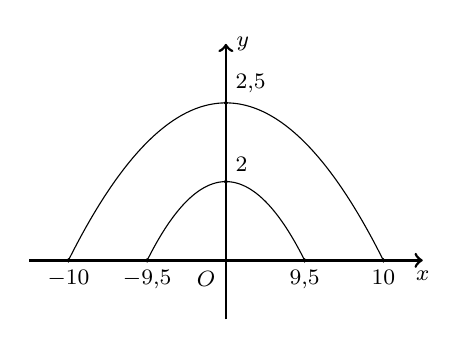
\begin{tikzpicture}[font=\footnotesize,scale=0.5]
\draw[->,line width = 1pt] (-5,0) --(0,0) node[below left]{$O$}--(5,0) node[below]{$x$};
\draw[->,line width = 1pt] (0,-1.5) --(0,5.5) node[right]{$y$};
\draw (0,4)  circle (1pt);
\draw (0,4) node[above right]{$2{,}5$} circle (1pt);
\draw (0,2)  circle (1pt);
\draw (0,2) node[above right]{$2$} circle (1pt);
\draw (4,0)  circle (1pt);
\draw (- 4,0)  circle (1pt);
\draw (4,0) node[below]{$10$} circle (1pt);
\draw (- 4,0) node[below]{$-10$} circle (1pt);
\draw (2,0)  circle (1pt);
\draw (- 2,0)  circle (1pt);
\draw (2,0) node[below]{$9{,}5$} circle (1pt);
\draw (- 2,0) node[below]{$-9{,}5$} circle (1pt);
\draw [samples=100, domain= - 4: 4] plot (\x, {(-0.25* (\x)^2) + 4});
\draw [samples=100, domain= - 2: 2] plot (\x, {(-0.5* (\x)^2) + 2});
\end{tikzpicture}
\end{center}
Gọi $({\mathrm{P}_1})\colon y={a_1}{x^2}+{b_1}$ là Parabol đi qua hai điểm $A(\dfrac{19}{2};0),B(0;2)$.\\
Nên ta có hệ phương trình
$\heva{& 0=a\cdot {{( \frac{19}{2} )}^2}+2 \\ & 2=b }
\Leftrightarrow \heva{& {a_1}=-\frac{8}{361} \\ & {b_1}=2 }
\Rightarrow ( {\mathrm{P}_1} )\colon y=-\frac{8}{361}{x^2}+2$.\\
Gọi $({\mathrm{P}_2})\colon y={a_2}{x^2}+{b_2}$ là Parabol đi qua hai điểm $C( 10;0 ),D( 0;\frac{5}{2} )$.\\
Nên ta có hệ phương trình
$\heva{& 0={a_2}\cdot {{( 10 )}^2}+\frac{5}{2} \\ & \frac{5}{2}={b_2} }
\Leftrightarrow \heva{& {a_2}=-\frac{1}{40} \\ & {b_2}=\frac{5}{2} }
\Rightarrow ( {\mathrm{P}_2} )\colon y
=-\frac{1}{40}{x^2}+\frac{5}{2}$.\\
Gọi mặt phẳng $(P)$ vuông góc với trục $Ox$, thiết diện tạo bởi mặt phẳng $(P)$ với khối bê tông là hình chữ nhật có chiều dài bằng 5, chiều rộng bằng\\
$ h(x)=\heva{&  ( -\dfrac{1}{40}{x^2}+\dfrac{5}{2} )-( -\frac{8}{361}{x^2}+2 )=\dfrac{-41}{14440}{x^2}+\dfrac{1}{2} & , & -9{,}5\le x\le 9{,}5 \\ & -\dfrac{1}{40}{x^2}+\dfrac{5}{2} & ,\, & x\in [ -10;-9{,}5 ]\cup [ 9{,}5;10 ] }$.\\
Suy ra diện tích thiết diện là
$S(x)=\heva{&  5( \frac{-41}{14440}{x^2}+\frac{1}{2} ) & , & -9{,}5\le x\le 9{,}5 \\ & 5( -\frac{1}{40}{x^2}+\frac{5}{2} ) & ,\, & x\in [ -10;-9{,}5 ]\cup [ 9{,}5;10 ] }$.\\
Do đó $V=\int\limits_{-10}^{10}{S(x)}\mathrm{\,d}x$.\\
Vậy $V=\int\limits_{-10}^{-9{,}5}{5\cdot ( \dfrac{-1}{40}{x^2}+\frac{5}{2} )}\mathrm{\,d}x+\int\limits_{-9{,}5}^{9{,}5}{5\cdot ( \dfrac{-41}{14440}{x^2}+\dfrac{1}{2} )}\mathrm{\,d}x+\int\limits_{9{,}5}^{10}{5\cdot ( \dfrac{-1}{40}{x^2}+\dfrac{5}{2} )}\mathrm{\,d}x=40$.}
\end{ex}

\begin{ex}%[Dự án 12-EX-3-2026, Tran Nhu Cang]%[2D4C3-4]
Có một cốc nước thủy tinh hình trụ, bán kính trong lòng đáy cốc là $6$\,m, chiều cao lòng cốc là $10$\,cm đang đựng một lượng nước. Tính thể tích (đơn vị: cm$^3$) lượng nước trong cốc, biết khi nghiêng cốc nước vừa lúc khi nước chạm miệng cốc thì đáy mực nước trùng với đường kính đáy cốc.
\begin{center}
\begin{tikzpicture}[scale=0.75,line cap=round,line join=round,font=\footnotesize,>=stealth]
\def\h{4.45}
\def\a{1.5}
\def\b{0.6}
\path
(0,0) coordinate (O')
($(O')+(0,\h)$)  coordinate (O)
($(O)+(0:\a cm and \b cm)$) coordinate (M)
($(O)+(180:\a cm and \b cm)$) coordinate (N)
($(O')+(0:\a cm and \b cm)$) coordinate (M')
($(O')+(180:\a cm and \b cm)$) coordinate (N')
;
\draw (M)--(M') (N)--(N');
%\draw[dashed] (O)--(O');
\draw  (O) ellipse  (\a cm and \b cm);
\draw [fill=cyan!30,dashed] ($(M')+(0,.3*\h)$) arc (0:180:\a cm and \b cm)-- ($(N')+(0,.3*\h)$) arc (180:360:\a cm and \b cm);
\draw [fill=cyan!40] ($(M')+(0,.3*\h)$) arc (0:-180:\a cm and \b cm) -- (N') arc (180:360:\a cm and \b cm);
\draw [dashed,] (M') arc (0:180:\a cm and \b cm);
\draw  (M') arc (0:-180:\a cm and \b cm);
\foreach \x/\y in{}{\fill [black](\x) circle (1pt) ($(\x)+(\y:3mm)$) node {$\x$};}
\end{tikzpicture}
\hspace{2cm}
\begin{tikzpicture}[scale=0.75,line cap=round,line join=round,font=\footnotesize,>=stealth]
\def\h{4.45}
\def\a{1.5}
\def\b{0.7}
\pgfmathsetmacro{\t}{(\h*\h+\a*\a)};
\begin{scope}
\path
(0,0) coordinate (O')
%($(O)+(\a,0)$) coordinate (B)
($(O')+(0,\h)$) [rotate=-60] coordinate (O)
($(O)+(0:\a cm and \b cm)$) coordinate (M)
($(O)+(180:\a cm and \b cm)$) coordinate (N)
($(O')+(0:\a cm and \b cm)$) coordinate (M')
($(O')+(180:\a cm and \b cm)$) coordinate (N')
($(O)+(-45:\a cm and \b cm)$)[rotate=-60] coordinate (A)
($(O')+(-45:\a cm and \b cm)$)[rotate=-60] coordinate (A')
($(O')+(-85:\a cm and 0.9*\b cm)$) [rotate=-60]coordinate (P)
%($(O')+(260:\a cm and \b cm)$) [rotate=60]coordinate (Q)
($(O')!-1!(P)$) coordinate (Q)
;
\fill[cyan!40] (M)--(M')-- (M') [rotate=-60] arc (0:-90:\a cm and 0.9*\b cm)--(Q)--cycle;
\fill[cyan!30] (O')--(M)--(M) ..controls +(-60:0.3) and +(-30:0.5)..(Q)--cycle;
\fill[cyan!30] (O')--(M)--(M) ..controls +(60:0.3) and +(30:0.5)..(P)--cycle;
\draw[color=gray,dashed] (M)..controls +(60:0.3) and +(30:0.5)..(P);
\draw[color=gray] (M)..controls +(-60:0.2) and +(-30:0.5)..(Q);
\draw [dashed,rotate=-60] (M') arc (0:180:\a cm and 0.9*\b cm);
\draw [rotate=-60,thick] (M') arc (0:-180:\a cm and 0.9*\b cm);
\draw [rotate=-60,thick] (O) ellipse (\a cm and 0.9*\b cm);
\draw [thick](M)--(M') (N)--(N');
\draw[dashed] (P)--(Q) ;
\foreach \x/\y in{}{\fill [black](\x) circle (1pt) ($(\x)+(\y:3mm)$) node {$\x$};}
%\gvg[size=0.1](S,O,A);
\end{scope}
\end{tikzpicture}
\end{center}
\par
\shortans{240}
\loigiai{
Đặt $R=6$\,cm, $h=10$\,cm. Gán hệ trục tọa độ như hình vẽ.
\begin{center}
\begin{tikzpicture}[scale=0.35, font=\footnotesize, line join=round, line cap=round, >=stealth,
declare function={R=6; h=10;goc=80;b=0.5*R; xmin=0;xmax=2*R+3;ymin=0;ymax=h+4;}]
\path (0,0) coordinate (O)
(2*R,0) coordinate (M)
(M) arc (0:goc: R and b) coordinate (N)
(R,0) coordinate (I)
(R,h) coordinate (J)
($(I)!-1!(N)$)coordinate (D)
(0,h) coordinate (H)
($(I)!0.7!(D)$)coordinate (C)
($(O)+(C)-(I)$)coordinate (X);
\path[name path=e1](I)ellipse (R and b);
\path[name path=cx](C)--(X);
\path[name intersections={of =e1 and cx,by=B}];
\path(intersection of {C--B} and {O--$(O)+(-135:1cm)$})coordinate (Xt);
\path(intersection of {C--H} and {B--$(B)+(90:1cm)$})coordinate (A);
\fill[pattern=north east lines] (A)--(B)--(C)--cycle;
\draw[dashed] (O) arc (180:0:R and b) (N)--(D) (O)--(M) (N)--(H)--(D) (H)--(I) (B)--(C)--(H);
\path pic["\scriptsize $\alpha$", angle eccentricity=.5,draw,angle radius=12pt]{angle= H--I--O};
\draw (O) arc (180:360:R and b) (J)ellipse (R and b) (2*R,h)--(M)  (A)--(B) (Xt)--(B);
\draw[->] (M)--(xmax,0) node[shift={(-100:7pt)}]{$y$};
\draw[->] (0,ymin)--(0,ymax) node[shift={(-30:7pt)}]{$z$};
\draw[->] (O)--(-135:1.3*R) node[shift={(-30:7pt)}]{$x$};
\fill (O) circle (1pt) node[shift={(135:7pt)}]{$O$};
\fill (Xt) circle (1pt) node[shift={(180:7pt)}]{$x$};
% Các điểm trên trục x và y
\foreach \x/\goc in {A/180,B/-90,C/0}{
\fill (\x) circle (1pt) node[shift={(\goc:7pt)},font=\small]{$\x$};
}
\end{tikzpicture}
\end{center}
Một mặt phẳng tùy ý vuông góc với trục $Ox$ tại điểm $x$ ($-6\leq x\leq 6$) cắt vật thể theo thiết diện có diện tích là $S(x)$.\\
Ta thấy thiết diện đó là một tam giác vuông, giả sử là tam giác $ABC$ vuông tại $B$ như trong hình vẽ.\\
Ta có $S(x)=S_{ABC}=\dfrac{1}{2} AB\cdot BC=\dfrac{1}{2} BC^2\cdot \tan \alpha=\dfrac{1}{2} \big(R^2-x^2\big)\dfrac{h}{R}=\dfrac{5\big(36-x^2\big)}{6}$.\\
Vậy thể tích lượng nước trong cốc là $V=\displaystyle\int\limits_{-6}^6 S(x)\mathrm{\,d}x=\displaystyle\int\limits_{-6}^6\dfrac{5\big(36-x^2\big)}{6} \mathrm{\,d}x=240$\,(cm$^3$).
}
\end{ex}

\begin{ex}%[12-EX-3-2026, Lê Hồng Phi]%[2D4C3-4]
\immini{Một bể nước có thiết kế phía dưới là hình hộp chữ nhật có đáy là hình vuông cạnh $10$ m, chiều cao là $1$ m; phía trên là hình chóp cụt đều có đáy trên là hình vuông cạnh $15$ m. Tổng chiều cao của bể là $4$ m. Lúc đầu bể không có nước, người ta bơm nước vào bể với tốc độ không đổi là $5$ m$^3$/phút. Hỏi sau một giờ bơm thì tốc độ dâng lên của nước trong bể là bao nhiêu m/phút (làm tròn kết quả đến hàng phần trăm)?}{\begin{tikzpicture}[scale=1, font=\footnotesize, line join=round, line cap=round,>=stealth]
\path (0,1) coordinate (h) (0,0)coordinate (B)++(3,0) coordinate (C)++(0.8,0.8) coordinate (D) ($(B)+(D)-(C)$) coordinate (A);
\foreach \p in {A,B,C,D}\path ($(\p)+(h)$) coordinate (\p');
\path (B')++(130:1.5) coordinate (b)++(4.5,0) coordinate (c) ($(c)+(D')-(C')$) coordinate (d1) ($(c)!1.5!(d1)$) coordinate (d) ($(b)+(d)-(c)$) coordinate (a);
\draw (a)--(b)--(c)--(d)--cycle (d)--(D')--(D)--(C)--(B)--(B')--(b) (B')--(C')--(c) (C)--(C')--(D');
\draw[dashed] (B)--(A)--(D) (A)--(A')--(D') (a)--(A')--(B');
\path (a)--(d)node[above,pos=0.5]{$15$ m} (B)--(C)node[below,pos=0.5]{$10$ m} (B)--(B')node[left,pos=0.5]{$1$ m};
\draw[<->] ($(d)+(0.5,0)$)--++(0,-2.6)node[pos=0.5,fill=white]{$4$ m};
%\foreach \p/\g in {A/150,B/240,C/-60,D/0,A'/90,B'/180,C'/-30,D'/45} \fill[black] (\p) circle(1pt)+(\g:0.3) node{$\p$};
\end{tikzpicture}}
\shortans{$0{,}03$}
\loigiai{
Sau $1$ giờ ($60$ phút), lượng nước bơm vào là $V=5\cdot 60=300$ m$^3$.\\
Thể tích phần bể nước hình hộp chữ nhật bên dưới là $V_1=10\cdot 10\cdot 1=100$ m$^3$.\\
Như thế, sau $20$ phút thì lượng nước bơm vào đầy phần bể nước hình hộp chữ nhật.\\
Do đó, lượng nước nằm trong phần chóp cụt là $V_2=300-100=200$ m$^3$.\\
Phần chóp cụt có chiều cao $h_\text{chóp cụt}=4-1=3$ m, đáy nhỏ $10$ m, đáy lớn $15$ m.\\
Bài toán trở thành tìm tốc độ nước dâng lên trong bể nước hình chóp cụt tại thời điểm $40$ phút.\\
Gọi $h=h(t)$ (mét) là mực nước trong hình chóp cụt tại thời điểm $t$ phút.\\
Gọi $x$ là chiều cao mực nước tính từ đáy chóp cụt ($0\le x\le 3$).\\
Cạnh của mặt nước hình vuông tại độ cao $x$ là $a(x)=10+\dfrac{15-10}{3}x=10+\dfrac{5}{3}x$.\\
Diện tích mặt thoáng tại độ cao $x$ là $S(x)=\left(10+\dfrac{5}{3}x\right)^2$.\\
Thể tích nước trong chóp cụt đến độ cao $h$ là \[V(h)=\displaystyle\int\limits_0^hS(x)\,\mathrm{d}x=\int\limits_0^h\left(10+\dfrac{5}{3}x\right)^2\,\mathrm{d}x=\dfrac{1}{5}\left[\left(10+\dfrac{5}{3}h\right)^3-1\,000\right].\]
Suy ra thể tích nước trong chóp cụt ở thời điểm $t$ là $V(h(t))=\dfrac{1}{5}\left[\left(10+\dfrac{5}{3}h(t)\right)^3-1\,000\right]$.\\
Vào lúc $40$ phút thì lượng nước nằm trong phần chóp cụt là $200$ m$^3$ nên ta có phương trình \begin{eqnarray*}
\dfrac{1}{5}\left[\left(10+\dfrac{5}{3}h(40)\right)^3-1\,000\right]=200&\Leftrightarrow &\left(10+\dfrac{5}{3}h(40)\right)^3=2\,000\\
&\Leftrightarrow& h(40)=\dfrac{3}{5}\left(\sqrt[3]{2\,000}-10\right).
\end{eqnarray*}
Vì tốc độ bơm không đổi là $5$ m$^3$/phút nên ta có \[V(h(t))=5t\Leftrightarrow \dfrac{1}{5}\left[\left(10+\dfrac{5}{3}h(t)\right)^3-1\,000\right]=5t\Leftrightarrow \left(10+\dfrac{5}{3}h(t)\right)^3=25t+1\,000.\quad (*)\]
Đạo hàm $2$ vế của $(*)$ theo $t$ ta được
\[5\left[10+\dfrac{5}{3}h(t)\right]^2\cdot h'(t)=25\Rightarrow h'(t)=\dfrac{5}{\left[10+\dfrac{5}{3}h(t)\right]^2}.\]
Do đó, tốc độ dâng lên của nước trong bể phần chóp cụt tại thời điểm $40$ phút là \[h'(40)=\dfrac{5}{\left[10+\dfrac{5}{3}h(40)\right]^2}\approx 0{,}03 \text{m/phút}.\]
Vậy tốc độ dâng lên của nước trong bể sau một giờ bơm là $0{,}03$ m/phút.
}
\end{ex}

\begin{ex}%[2D4C3-5]
Trong chương trình nông thôn mới, tại một xã Y có xây một cây cầu bằng bê tông như hình vẽ. Tính thể tích khối bê tông để đổ đủ cây cầu. (Đường cong trong hình vẽ là các đường Parabol).
\shortans{$40$}
\begin{center}
\begin{tikzpicture}[scale=1.4, font=\footnotesize, line join=round, line cap=round,>=stealth,samples=100]
\path
(0,0) coordinate (O)
(-1,0) coordinate (B)
(0,1) coordinate (C)
(1,0) coordinate (D)
(-1.4,0) coordinate (M)
(0,1.96) coordinate (N)
(1.4,0) coordinate (P)
;
\path (-165:4) coordinate (A);
\foreach \x in {B,C,D,M,N,P,O}{\path ($(\x)+(-165:4)$) coordinate (\x_1);}
\fill[gray!40] (N_1)--(N)--plot[domain=0:1.4] (\x,{-(\x)^2+1.96})--(P)--(P_1)--plot[shift={(A)},domain=1.4:0] (\x,{-(\x)^2+1.96});
\fill[gray!40] (M_1)--plot[shift={(A)},domain=-1.4:1.4](\x,{-(\x)^2+1.96})--(P_1)--(D_1)--plot[shift={(A)},domain=1:-1] (\x,{-(\x)^2+1})--(B_1)--(M_1);
\draw[dash pattern=on 2pt off 2pt] plot[domain=-1:1] (\x,{-(\x)^2+1})
plot[domain=-1.4:1.4] (\x,{-(\x)^2+1.96})
(M)--(P) (O)--(N)
;
\draw[shift={(A)}] plot[domain=-1:1] (\x,{-(\x)^2+1});
\draw[shift={(A)}] plot[domain=-1.4:1.4] (\x,{-(\x)^2+1.96});
\draw [dash pattern=on 2pt off 2pt] (B)--(B_1) (C)--(C_1) (D)--(D_1) (M)--(M_1)
(O_1)--(N_1)
;
\draw (N)--(N_1) (P)--(P_1) (M_1)--(P_1);
\foreach \t in {O,B,M,P,O_1,M_1,B_1,D_1,P_1}{
\draw[fill=white] (\t) circle (1pt);}
\path (M_1)--(B_1) node[midway,below]{$0,5$m};
\path (B_1)--(D_1) node[midway,below]{$19$m};
\path (D_1)--(P_1) node[midway,below]{$0,5$m};
\path (O)--(C) node[midway,right]{$2$m};
\path (C)--(N) node[pos=0.2,left]{$0,5$m};
\end{tikzpicture}
\end{center}
\loigiai{
Chọn hệ trục $Oxy$ như hình vẽ.
\begin{center}
\begin{tikzpicture}[scale=1.4, font=\footnotesize, line join=round, line cap=round,>=stealth,samples=100]
\path
(0,0) coordinate (O)
(-1,0) coordinate (B)
(0,1) coordinate (C)
(1,0) coordinate (D)
(-1.4,0) coordinate (M)
(0,1.96) coordinate (N)
(1.4,0) coordinate (P)
;
\path (-165:4) coordinate (A);
\foreach \x in {B,C,D,M,N,P,O}{\path ($(\x)+(-165:4)$) coordinate (\x_1);}
\fill[gray!40] (N_1)--(N)--plot[domain=0:1.4] (\x,{-(\x)^2+1.96})--(P)--(P_1)--plot[shift={(A)},domain=1.4:0] (\x,{-(\x)^2+1.96});
\fill[gray!40] (M_1)--plot[shift={(A)},domain=-1.4:1.4](\x,{-(\x)^2+1.96})--(P_1)--(D_1)--plot[shift={(A)},domain=1:-1] (\x,{-(\x)^2+1})--(B_1)--(M_1);
\draw[-stealth,dash pattern=on 2pt off 2pt] (-1.4,0)--(0,0)node[below left]{$O$}--(2,0) node[below] {$x$};
\draw[-stealth,dash pattern=on 2pt off 2pt] (0,0)--(0,2.5) node[left] {$y$};
\draw[dash pattern=on 2pt off 2pt] plot[domain=-1:1] (\x,{-(\x)^2+1})
plot[domain=-1.4:1.4] (\x,{-(\x)^2+1.96})
;
\draw[shift={(A)}] plot[domain=-1:1] (\x,{-(\x)^2+1});
\draw[shift={(A)}] plot[domain=-1.4:1.4] (\x,{-(\x)^2+1.96});
\draw [dash pattern=on 2pt off 2pt] (B)--(B_1) (C)--(C_1) (D)--(D_1) (M)--(M_1)
(O_1)--(N_1)
;
\draw (N)--(N_1) (P)--(P_1) (M_1)--(P_1);
\foreach \t in {O,B,M,P,O_1,M_1,B_1,D_1,P_1}{
\draw[fill=white] (\t) circle (1pt);}
\path (M_1)--(B_1) node[midway,below]{$0,5$m};
\path (B_1)--(D_1) node[midway,below]{$19$m};
\path (D_1)--(P_1) node[midway,below]{$0,5$m};
\path (O)--(C) node[midway,right]{$2$m};
\path (C)--(N) node[pos=0.2,left]{$0,5$m};
\end{tikzpicture}
\end{center}
Gọi $(P_1)\colon y=a_1x^2+b_1$ là Parabol đi qua hai điểm $A\left(\dfrac{19}{2};0\right)$, $B\left(0;2\right)$.\\
Nên ta có hệ phương trình sau $\heva{& 0=a\cdot \left(\dfrac{19}{2}\right)^2+2\\
&2=b}\Leftrightarrow \heva{
&a_1=-\dfrac{8}{361}\\
&b_1=2} \Rightarrow (P_1)\colon y=-\dfrac{8}{361}{x^2}+2$.\\
Gọi $\left(P_2\right)\colon y=a_2x^2+b_2$ là Parabol đi qua hai điểm $C(10;0)$, $D\left(0;\dfrac{5}{2}\right)$.\\
Nên ta có hệ phương trình sau $\heva{
& 0=a_2\cdot (10)^2+\dfrac{5}{2}\\
&\dfrac{5}{2}=b_2}\Leftrightarrow \heva{
&{a_2}=-\dfrac{1}{40}\\
&{b_2}=\dfrac{5}{2}} \Rightarrow \left(P_2\right)\colon y=-\dfrac{1}{40}x^2+\dfrac{5}{2}$.\\
Ta có thể tích của bê tông là $V=5\cdot 2\left[\displaystyle\int\limits_0^{10}\left(-\dfrac{1}{40}x^2+\dfrac{5}{2}\right)\mathrm{\,d}x-\displaystyle\int\limits_0^{\tfrac{19}{2}}\left(-\dfrac{8}{361}x^2+2\right)\mathrm{\,d}x\right]=40$ m$^3$.
}
\end{ex}

\begin{ex}%[2D4C3-5]
Một chi tiết máy được thiết kế như hình vẽ bên.
\shortans{$17{,}7$}
\begin{center}
\begin{tikzpicture}[scale=1, font=\footnotesize, line join=round, line cap=round,>=stealth,declare function={a=3;h=4.5;}]
\path (0,0) coordinate (A)
--++(30:a) coordinate (B)
--++(90:a) coordinate (C)
($(A)+(C)-(B)$) coordinate (D)
($(A)+(180:h)$) coordinate (F)
($(B)+(F)-(A)$) coordinate (E)
($(D)+(180:a)$) coordinate (P)
($(C)+(P)-(D)$) coordinate (Q)
;
\draw (A)--(B)--(C)--(D)--cycle (F)--(A) (D)--(P)--(Q)--(C);
\draw[dashed] (F)--(E)--(B);
\draw (F)..controls +(30:1) and +(-100:1)..(P)node[midway,right]{$c$};
\draw[dashed] (E)..controls +(30:1) and +(-100:1)..(Q)node[pos=0.3,right]{$c$};
\foreach \t/\g in {A/-90,B/-90,C/0,D/-45,E/135,F/-90,P/180,Q/135}{
\draw[fill=black] (\t) circle (1pt) node[shift={(\g:7pt)},font=\scriptsize]{$ \t $};
}
\end{tikzpicture}
\end{center}
Các tứ giác $ABCD$, $CDPQ$ là các hình vuông cạnh $2{,}5$ (cm). Tứ giác $ABEF$ là hình chữ nhật có $BE=3{,}5$ (cm). Mặt bên $PQEF$ được mài nhẵn theo đường parabol $(P)$ có đỉnh parabol nằm trên cạnh $ EF$. Thể tích của chi tiết máy bằng bao nhiêu? (viết kết quả dưới dạng số thập phân và làm tròn đến hàng phần mười)
\loigiai{\begin{center}
\begin{tikzpicture}[scale=1, font=\footnotesize, line join=round, line cap=round,>=stealth,declare function={a=3;h=6;}]
\path (0,0) coordinate (A)
--++(30:a) coordinate (B)
--++(90:a) coordinate (C)
($(A)+(C)-(B)$) coordinate (D)
($(A)+(180:h)$) coordinate (F)
($(B)+(F)-(A)$) coordinate (E)
($(D)+(180:a)$) coordinate (P)
($(C)+(P)-(D)$) coordinate (Q)
($(A)+(P)-(D)$) coordinate (S)
($(B)+(Q)-(C)$) coordinate (R)
($(F)!0.5!(S)$) coordinate (M)
($(M)+(90:2)$) coordinate (M_1)
($(E)!0.5!(R)$) coordinate (K)
($(K)+(90:2)$) coordinate (K_1)
;
\path[name path=d1] (F)..controls +(30:1) and +(-100:1)..(P);
\path[name path=d2] (E)..controls +(30:1) and +(-100:1)..(Q);
\path[name path=d3] (M)--(M_1);
\path[name path=d4] (K)--(K_1);
\path[name intersections={of=d1 and d3,by=N}];
\path[name intersections={of=d2 and d4,by=H}];
\fill[gray!30] (N)--(M)--(K)--(H)--cycle;
\draw (A)--(B)--(C)--(D)--cycle (F)--(A) (D)--(P)--(Q)--(C) (P)--(S) (N)--(M);
\draw[dashed] (F)--(E)--(B) (Q)--(R)--(S) (M)--(K)--(H) (N)--(H);
\draw (F)..controls +(30:1) and +(-100:1)..(P);
\draw[dashed] (E)..controls +(30:1) and +(-100:1)..(Q);
\draw[-stealth] (A)--++(0:1)node[below]{$x$};
\draw[-stealth] (F)--++(90:1.5*a)node[left]{$y$};
\foreach \t/\g in {A/-90,B/-90,C/0,D/-45,E/115,F/-90,P/180,Q/135,S/-90,R/-90,N/90,M/-90,K/-90,H/135}{
\draw[fill=black] (\t) circle (1pt) node[shift={(\g:7pt)},font=\scriptsize]{$ \t $};
}
\end{tikzpicture}
\end{center}
Gọi hình chiếu của $P$, $Q$ trên $AF$ và $BE$ là $S$ và $R$. Vật thể được chia thành hình lập phương $ABCD.PQRS$ có cạnh $2{,}5$ (cm), thể tích $V_1=\dfrac{125}{8}$ cm$^3$ và phần còn lại có thể tích $V_2$. Khi đó thể tích vật thể $V=V_1+V_2=\dfrac{125}{8}+V_2$.\\
Đặt hệ trục $Oxyz$ sao cho $O$ trùng với $F$, $Ox$ trùng với $FA$, $Oy$ trùng với tia $Fy$ song song với $AD$. Khi đó Parabol $(P)$ có phương trình dạng $y=ax^2$, đi qua điểm $P\left(1;\dfrac{5}{2}\right)$ do đó $a=\dfrac{5}{2}\Rightarrow y=\dfrac{5}{2}{x^2}$.\\
Cắt vật thể bởi mặt phẳng vuông góc với $Ox$ và đi qua điểm $M(x;0;0)$, $0\le x\le 1$ ta được thiết diện là hình chữ nhật $MNHK$ có cạnh là $ MN=\dfrac{5}{2}x^2$ và $ MK=\dfrac{5}{2}$ do đó diện tích $S(x)=\dfrac{25}{4}x^2$.\\
Áp dụng công thức thể tích vật thể ta có $V_2=\displaystyle\int\limits_0^1\dfrac{25}{4}x^2\mathrm{\,d}x=\dfrac{25}{12}$.\\
Từ đó $V=\dfrac{125}{8}+\dfrac{25}{12}=\dfrac{425}{24}\approx17{,}7$ cm$^3$.
}
\end{ex}

\begin{ex}%[2D4C3-5]
Cho một mô hình $3-D$ mô phỏng một đường hầm như hình vẽ bên. Biết rằng đường hầm mô hình có chiều dài $5$ (cm); khi cắt hình này bởi mặt phẳng vuông góc với đáy của nó, ta được mặt cắt là một hình parabol có độ dài đáy gấp đôi chiều cao parabol. Chiều cao của mỗi mặt cắt hình parabol cho bởi công thức $ y=3-\dfrac{2}{5}x$ (cm), với $x$ (cm) là khoảng cách tính từ lối vào lớn hơn của đường hầm mô hình. Tính thể tích (theo đơn vị cm$^3$) không gian bên trong đường hầm mô hình (làm tròn kết quả đến hàng đơn vị).
\shortans{$29$}
\begin{center}
\begin{tikzpicture}[scale=1,declare function={a=0.8;b=0.6;c=0.4;d=0.2;}]
\tikzset{
homothety at/.style args={#1 scaled by #2}{shift={($(#1)!#2!(0,0)$)},scale=#2},
}
\def\mypath{(-120:2)..controls +(90:0.6) and +(-180:0.6)..(0,3)}
\def\mydot{(0,3)..controls +(0:0.25) and +(95:0.05)..(60:2)}
\draw \mypath;
\draw[dashed] \mydot;
\path (7,0) coordinate (c1);
\begin{scope}[homothety at=c1 scaled by a]
\draw \mypath;
\draw[dashed] \mydot;
\end{scope}
\begin{scope}[homothety at=c1 scaled by b]
\draw \mypath;
\draw[dashed] \mydot;
\end{scope}
\begin{scope}[homothety at=c1 scaled by c]
\draw \mypath;
\draw[dashed] \mydot;
\end{scope}
\begin{scope}[homothety at=c1 scaled by d]
\draw \mypath;
\draw \mydot;
\end{scope}
\path
(-120:2) coordinate (A)
(0,3) coordinate (B)
(60:2) coordinate (C);
\foreach \x in {A,B,C}{\path ($(c1)!a!(\x)$) coordinate (\x_1);}
\foreach \x in {A,B,C}{\path ($(c1)!b!(\x)$) coordinate (\x_2);}
\foreach \x in {A,B,C}{\path ($(c1)!c!(\x)$) coordinate (\x_3);}
\foreach \x in {A,B,C}{\path ($(c1)!d!(\x)$) coordinate (\x_4);}
\path ($(A_4)!0.5!(B_4)$) coordinate (D);
\draw (A)--(A_4) (B)--(B_4) (A_4)--(C_4)
;
\draw[dashed] (B)node[above]{$3$}--(O)--(D)node[below right]{$5$} (A)--(C) (A_1)--(C_1) (A_2)--(C_2) (A_3)--(C_3)  (C)--(C_4);
\end{tikzpicture}
\end{center}
\loigiai{
\begin{center}
\begin{tikzpicture}[scale=1,font=\footnotesize]
\path (0,0) coordinate (O)
(2,0) coordinate (A)
(0,2) coordinate (B)
;
\draw[-stealth] (-3.5,0)--(0,0)--(3,0)node[below]{$x$};
\draw[-stealth] (0,-1.5)--(0,4)node[left]{$y$};
\draw[smooth,samples=100] plot[domain=-2:2](\x,{(-1/2)*(\x)^2+2});
\foreach \x in {O,A,B}{\draw[fill=blue!40] (\x) circle (1pt);}
\foreach \x in {-3,-2,-1,1}{\draw (\x,0.05)--(\x,-0.05);}
\foreach \x in {-1,1,3}{\draw (-0.05,\x)--(0.05,\x);}
\node[above left] at (B) {$h$};
\path (O)--(A)node[below]{$h$};
\node at (0,0) [below left]{$O$};
\end{tikzpicture}
\end{center}
Xét một mặt cắt hình parabol có chiều cao là $h$ và độ dài đáy $2h$ và chọn hệ trục $Oxy$ như hình vẽ trên.\\
Parabol $(P)$ có phương trình $(P)\colon y=ax^2+h$, $(a<0)$.\\
Có $B(h;0)\in(P)\Leftrightarrow 0=ah^2+h\Leftrightarrow a=-\dfrac{1}{h}$ (do $h>0$).\\
Diện tích $S$ của mặt cắt là \[S=\displaystyle\int\limits_{-h}^h\left(-\dfrac{1}{h}{x^2}+h\right)\mathrm{\,d}x=\dfrac{4h^2}{3}, h=3-\dfrac{2}{5}x.\]
$\Rightarrow S(x)=\dfrac{4}{3}{\left(3-\dfrac{2}{5}x\right)^2}.$\\
Suy ra thể tích không gian bên trong của đường hầm mô hình
\[ V=\displaystyle\int\limits_0^5S(x)\mathrm{\,d}x=\displaystyle\int\limits_0^5\dfrac{4}{3}\left(3-\dfrac{2}{5}x\right)^2\mathrm{\,d}x=\dfrac{260}{9}\approx 29\,\left(\text{cm}^3\right).\]
}
\end{ex}

\begin{ex}%[2D4C3-5]
Cho chiếc trống như hình vẽ, có đường sinh là nửa elip được cắt bởi trục lớn với độ dài trục lớn bằng $80$ cm, độ dài trục bé bằng $60$ cm và đáy trống là hình tròn có bán kính bằng $60$ cm. Tính thể tích $V$ của chiếc trống (đơn vị tính theo đề-xi-mét và kết quả làm tròn đến hàng đơn vị).
\shortans{$345$}
\begin{center}
\begin{tikzpicture}[scale=0.6,declare function={r=3;h=8;}]
\path (0:0) coordinate (O)
(-r,0) coordinate (A)
(r,0) coordinate (B)
;
\foreach \x in {O,A,B}{\path ($(\x)+(-100:h/2)$) coordinate (\x_1);}
\foreach \x in {O,A,B}{\path ($(\x)+(-90:h)$) coordinate (\x_2);}

\draw (A) arc (180:-180:{r} and {r/3})
(A_2) arc (180:360:{r} and {r/3})
(O)--(B)
;
\draw[dashed] (A_2) arc(180:0:{r} and {r/3})
(O)--(O_2) (O_2)--(B_2)node[midway,above]{$60$ cm}
;
\draw[-stealth] (B_1)--++(0:1)node[right]{\text{đường sinh}};
\draw[smooth,samples=100] (3,0)..controls +(-100:1) and  +(90:2)..(2,-4)..controls +(-90:2) and +(100:1.5)..(3,-8)
;
\draw[xscale=-1,smooth,samples=100] (3,0)..controls +(-100:1) and  +(90:2)..(2,-4)..controls +(-90:2) and +(100:1.5)..(3,-8)
;
\end{tikzpicture}
\end{center}
\loigiai{
Đặt hệ trục tọa độ $Oxy$ như hình vẽ (trục hoành là trục của chiếc trống, gốc tọa độ là trung điểm của đường cao chiếc trống, đơn vị (dm).
\begin{center}
\begin{tikzpicture}[font=\footnotesize,scale=0.6,declare function={r=3;h=8;}]
\path (0:0) coordinate (O)
(h/2,0) coordinate (I)
(h/2,r) coordinate (A)
(h/2,-r) coordinate (B)
;
\foreach \x in {I,A,B}{\path ($(\x)+(180:h)$) coordinate (\x_1);}

\draw (A) arc (90:-90:{r/3} and {r})
(A_1) arc (90:450:{r/3} and {r})
(I_1)--(A_1)
;
\draw[dashed] (A) arc (90:270:{r/3} and {r})
;
\draw[smooth,samples=100] (4,3)..controls +(-168:0.5) and +(0:2)..(0,2.2)..controls +(180:2) and +(-12:0.5)..(-4,3);
\draw[yscale=-1,smooth,samples=100] (4,3)..controls +(-168:0.5) and +(0:2)..(0,2.2)..controls +(180:2) and +(-12:0.5)..(-4,3);
\draw[dashed] (I_1)--(O)node[below]{$O$}--(I)--(A)node[midway,right]{$6$} (O)--(0,2.2);
\draw[-stealth] (I)--++(0:2)node[below]{$x$};
\draw[-stealth] (0,2.2)--++(90:2)node[right]{$y$};
\end{tikzpicture}
\end{center}
Gọi $(E)$ là elip có phương trình $\dfrac{x^2}{16}+\dfrac{y^2}{9}=1$ thì ảnh của $(E)$ qua phép tịnh tiến theo vectơ $\vec{u}=(0 ; 6)$ là elip $\left(E^{\prime}\right)$ có phương trình $\dfrac{x^2}{16}+\dfrac{(y-6)^2}{9}=1$.\\
Suy ra, phương trình của đường sinh là $y=6-\dfrac{3}{4} \sqrt{16-x^2}$.\\
Do đó, thể tích của chiếc trống là $V=\pi \displaystyle\int\limits_{-4}^4\left(6-\dfrac{3}{4} \sqrt{16-x^2}\right)^2 \mathrm{\,d}x \approx 345$ dm$^3$.
}
\end{ex}

\begin{ex}%[2D4C3-5]
Chuẩn bị cho đêm hội diễn văn nghệ chào đón năm mới, bạn An đã làm một chiếc mũ \lq\lq cách điệu\rq\rq~cho ông già Noel có dáng một khối tròn xoay. Mặt cắt qua trục của chiếc mũ như hình vẽ bên dưới. Biết rằng $OO'=5$ cm, $OA=10$ cm, $OB=20$ cm, đường cong $AB$ là một phần của parabol có đỉnh là điểm $A$. Thể tích của chiếc mũ bằng bao nhiêu? (kết quả làm tròn đến hàng đơn vị)
\shortans{$2618$}
\begin{center}
\begin{tikzpicture}[line join=round, line cap=round,>=stealth,scale=0.2]
\path (0,0) coordinate (O)
(10,0) coordinate (A)
(0,20) coordinate (B)
(0,-5) coordinate (O')
(10,-5) coordinate (I)
(-10,-5) coordinate (C)
(-10,0) coordinate (D)
;
\draw[smooth,samples=100,thick] plot[domain=0:10](\x,{(1/5)*((\x)-10)^2})
plot[domain=-10:0](\x,{(1/5)*((\x)+10)^2})
;
\draw[dash pattern=on 2pt off 2pt] (O')--(O)--(B) (A)--(D);
\draw[thick] (A)--(I)--(C)--(D);
\foreach \t/\g in {A/90,B/45,O/-135,O'/-135}{
\draw[fill=black] (\t) circle (1pt) node[shift={(\g:7pt)},font=\scriptsize]{$ \t $};
}
\end{tikzpicture}
\end{center}
\loigiai{
\begin{center}
\begin{tikzpicture}[line join=round, line cap=round,>=stealth,font=\scriptsize,scale=0.2]
\path (0,0) coordinate (O)
(10,0) coordinate (A)
(0,20) coordinate (B)
(0,-5) coordinate (O')
(-10,0) coordinate (C)
;
\draw[-stealth] (-12,0)--(0,0)--(12,0)node[below]{$x$};
\draw[-stealth] (0,-7)--(0,22)node[left]{$y$};
\draw[smooth,samples=100,thick] plot[domain=0:10](\x,{(1/5)*((\x)-10)^2})
plot[domain=-10:0](\x,{(1/5)*((\x)+10)^2})
;
\draw[thick] (10,0) rectangle (-10,-5);
\foreach \t/\g in {O/-135,O'/-135}{
\draw[fill=black] (\t) circle (1pt) node[shift={(\g:7pt)},font=\scriptsize]{$ \t $};
}
\draw[fill=black] (A) circle (1pt)node[shift={(45:10pt)}]{$A(10;0)$};
\draw[fill=black] (B) circle (1pt)node[right]{$B(0;20)$};
\path (O')--(O)node[pos=0.4,left]{$5$};
\node at ($(A)+(100:10)$) {$y=\dfrac{1}{5}(x-10)^2$};
\end{tikzpicture}
\end{center}
Ta gọi thể tích của chiếc mũ là $V$.\\
Thể tích của khối trụ có bán kính đáy bằng $ OA=10$ cm và đường cao $OO'=5$ cm là $V_1$.\\
Thể tích của vật thể tròn xoay khi quay hình phẳng giới hạn bởi đường cong $ AB$ và hai trục tọa độ quanh trục $ Oy$ là $V_2$.\\
Ta có $ V=V_1+V_2$\\
$V_1=5\cdot 10^2\pi=500\pi$ (cm$^3$).\\
Chọn hệ trục tọa độ như hình vẽ.\\
Do parabol có đỉnh $ A$ nên nó có phương trình dạng $ (P)\colon y=a(x-10)^2$.\\
Vì $(P)$ qua điểm $B(0;20)$ nên $ a=\dfrac{1}{5}$.\\
Do đó, $(P)\colon y=\dfrac{1}{5}(x-10)^2$. Từ đó suy ra $ x=10-\sqrt{5y}$ (do $ x<10$).\\
Suy ra $V_2=\pi\displaystyle\int\limits_0^{20}\left(10-\sqrt{5y}\right)^2 \mathrm{\,d}y=\pi\left(3000-\dfrac{8000}{3}\right)=\dfrac{1000}{3}\pi$ (cm$^3$).\\
Do đó $ V=V_1+V_2=500\pi+\dfrac{1000}{3}\pi=\dfrac{2500}{3}\pi$ (cm$^3$) $\approx2618$ (cm$^3$).
}
\end{ex}

\begin{ex}%[2-GHK2-1-ChuyenViThanh-HauGiang-25]%[12-EX-3-2026, Tran Quoc]%[2D4C3-5]
Từ một tấm bìa hình vuông $ABCD$ cạnh $4$\,cm, ta vẽ hai đường chéo và hai nửa đường tròn đường kính là hai cạnh $AD$, $BC$ cắt nhau tạo thành $4$ hình cánh quạt như hình vẽ sau:
\begin{center}
\begin{tikzpicture}[font=\footnotesize, line join=round, line cap=round, >=stealth, scale=1]
\coordinate (D) at (0,0);
\coordinate (C) at (4,0);
\coordinate (B) at (4,4);
\coordinate (A) at (0,4);
\coordinate (O) at (2,2);
\begin{scope}
\clip (A) -- (O) -- (B) -- cycle;
\fill[gray!80] (0,2) circle (2);
\fill[gray!80] (4,2) circle (2);
\end{scope}
\begin{scope}
\clip (C) -- (O) -- (D) -- cycle;
\fill[gray!80] (0,2) circle (2);
\fill[gray!80] (4,2) circle (2);
\end{scope}
\begin{scope}
\clip (D) -- (A) -- (B) -- (C) -- cycle;
\draw (0,2) circle(2) (4,2) circle(2);
\end{scope}
\draw (A) -- (B) -- (C) -- (D) -- cycle (A) -- (C) (B) -- (D);
\foreach \x/\pos in {A/135, B/45, C/-45, D/-135} \fill (\x) circle (1.5pt) node[shift=(\pos:0.25)] {$\x$};
\end{tikzpicture}
\end{center}
Tính thể tích khối tròn xoay sinh ra khi quay $4$ cánh quạt này quanh cạnh $CD$ (kết quả làm tròn đến hàng phần mười).
\par\shortans{57,4}
\loigiai{
Chọn hệ trục tọa độ $Oxy$ như hình vẽ sau:
\begin{center}
\begin{tikzpicture}[font=\footnotesize, line join=round, line cap=round, >=stealth, scale=1]
\coordinate (D) at (0,0);
\coordinate (C) at (4,0);
\coordinate (B) at (4,4);
\coordinate (A) at (0,4);
\coordinate (O) at (2,2);
\begin{scope}
\clip (A) -- (O) -- (B) -- cycle;
\fill[gray!80] (0,2) circle (2);
\fill[gray!80] (4,2) circle (2);
\end{scope}
\begin{scope}
\clip (C) -- (O) -- (D) -- cycle;
\fill[gray!80] (0,2) circle (2);
\fill[gray!80] (4,2) circle (2);
\end{scope}
\begin{scope}
\clip (D) -- (A) -- (B) -- (C) -- cycle;
\draw (0,2) circle(2) (4,2) circle(2);
\end{scope}
\draw (A) -- (B) -- (C) -- (D) -- cycle (A) -- (C) (B) -- (D);
\foreach \x/\pos in {A/135, B/45, C/-45, D/-90} \fill (\x) circle (1.5pt) node[shift=(\pos:0.25)] {$\x$};
\draw[->] (0,0)--(5.5,0) node[shift=(-110:0.2)] {$x$};
\draw[->] (0,0)--(0,5.5) node[shift=(-150:0.2)] {$y$};
\fill (0,0) circle(1pt) node[shift=(180:0.2)]{$O$};
\fill (2,0) circle(1pt) node[shift=(-90:0.2)]{$2$};
\fill (0,2) circle(1pt) node[shift=(180:0.2)]{$2$};
\fill (2,2) circle(1pt);
\draw[dashed] (2,0)|-(0,2);
\end{tikzpicture}
\end{center}
Do tính chất đối xứng, thể tích khối tròn xoay cần tìm bằng $2$ lần thể tích khối tròn xoay tạo thành khi quay phần cánh quạt bên trái quanh trục $Ox$. \\
Phương trình các đường chéo là $BD \colon y=x$ và $AC\colon y=-x+4$.\\
Nửa đường tròn đường kính $AD$ có phương trình là
\[x=\sqrt{4-(y-2)^2} \Rightarrow y = 2 \pm \sqrt{4-x^2}.\]
Suy ra phần thể tích khối tròn xoay được tạo thành là
\[\displaystyle  V=2\pi\left[\int\limits_{0}^{2}\left(\left(2+\sqrt{4-x^2}\right)^2-(-x+4)^2\right)\mathrm{\, d} x+\int\limits_{0}^{2}\left(x^2-\left(2-\sqrt{4-x^2}\right)^2\right)\mathrm{\, d} x\right] \approx 57{,}4\,\left(\text{cm}^3\right). \]
}
\end{ex}

\begin{ex}%[12-EX-3-2026, Dương Quang]%[2D4C3-5]
Giả sử bạn có hai chiếc cốc cà phê $C_1$ và $C_2$ như hình minh họa, một chiếc phình ra ngoài và một chiếc lõm vào trong. Bạn nhận thấy rằng chúng có cùng chiều cao và hình dạng của chúng khớp nhau hoàn hảo. Bạn tự hỏi tỉ lệ thể tích của hai chiếc cốc $\dfrac{V_{C_1}}{V_{C_2}}$ bằng bao nhiêu? Tất nhiên, bạn có thể đổ đầy nước vào một chiếc cốc rồi rót sang chiếc còn lại để so sánh, nhưng với tư cách là một học sinh vừa học xong các ứng dụng của tích phân, bạn quyết định tiếp cận theo hướng toán học hơn. Bỏ qua phần tay cầm, coi độ dày của cốc không đáng kể, bạn nhận thấy rằng phần bên trong của cả hai chiếc cốc đều tạo bởi các mặt quay quanh trục. Cụ thể, $C_1$ do hình phẳng $ABMIN$ quay quanh $AB$, $C_2$ do hình phẳng $DCMIN$ quay quanh $CD$. Biết rằng $ABCD$ là hình vuông cạnh $10$\,cm, $M$, $N$ lần lượt thuộc hai cạnh $BC$, $AD$ sao cho $MN\parallel AB$, $BM=4$\,cm. Điểm $K$ là trung điểm của $AB$ và $I$ là tâm của hình vuông $ABCD$. Cung $MIN$ là một phần của parabol nhận $I$ là đỉnh. Tỉ số $\dfrac{V_{C_1}}{V_{C_2}}$ bằng $\dfrac{a}{b}$, trong đó $a$, $b \in \mathbb{N}$, $\dfrac{a}{b}$ là phân số tối giản. Tính $a+b$.
\begin{center}
\begin{tikzpicture}[scale=.4, font=\footnotesize, line join=round, line cap=round, >=stealth,rotate=-90]
\foreach \x/\y/\t in {0/0/K,5/0/A,-5/0/B,-5/10/C,5/10/D,-5/4/M,5/4/N,0/5/I,0/10/Q}{
\path (\x,\y) coordinate (\t);
}
\fill[red!20](A)--(B)--(C)--(D)--cycle;
\fill[cyan!50](A)--(B)--(M)-- plot[samples=200,domain=-5:5,smooth,variable=\x] (\x,{-0.04*((\x)^2)+5})--(N)--cycle;
\draw [samples=200,domain=-5:5,smooth,variable=\x] plot (\x,{-0.04*((\x)^2)+5});
\draw (A)--(B)--(C)--(D)--cycle;
\draw[dashed] (M)--(K)--(N)--cycle (K)--(I);
\path (K)--(I) node[midway,above] {$C_1$};
\path (I)--(Q) node[midway,above] {$C_2$};
\foreach \t/\g in {A/-90,B/90,C/90,D/-90,K/180,I/45,M/90,N/-90}{
\fill (\t) circle (1pt) node[shift={(\g:7pt)},font=\scriptsize]{$ \t $};
}
\end{tikzpicture}
\end{center}
\shortans[]{$189$}
\loigiai{

\begin{itemize}
\item Tính thể tích của cốc $1$.\\
\begin{center}
\begin{tikzpicture}[scale=.4, font=\footnotesize, line join=round, line cap=round, >=stealth,rotate=-90]
\foreach \x/\y/\t in {0/0/K,5/0/A,-5/0/B,-5/10/C,5/10/D,-5/4/M,5/4/N,0/5/I,0/10/Q}{
\path (\x,\y) coordinate (\t);
}
\fill[red!20](A)--(B)--(C)--(D)--cycle;
\fill[cyan!50](A)--(B)--(M)-- plot[samples=200,domain=-5:5,smooth,variable=\x] (\x,{-0.04*((\x)^2)+5})--(N)--cycle;
\draw[->] (-2,0)--(6,0) node[shift={(180:7pt)}] {$x$};
\draw[->] (0,-3.5)--(0,11) node[shift={(90:7pt)}]{$y$};
\draw [samples=200,domain=-5:5,smooth,variable=\x] plot (\x,{-0.04*((\x)^2)+5});
\draw (A)--(B)--(C)--(D)--cycle;
\draw[dashed] (M)--(K)--(N)--cycle (K)--(I);
\path (K)--(I) node[midway,above] {$C_1$};
\path (I)--(Q) node[midway,above] {$C_2$};
\foreach \t/\g in {A/180,B/90,C/90,D/-90,K/135,I/45,M/90,N/-90}{
\fill (\t) circle (1pt) node[shift={(\g:7pt)},font=\scriptsize]{$ \t $};
}
\end{tikzpicture}
\end{center}
Chọn hệ trục tọa độ như hình vẽ, từ giả thiết bài toán suy ra $K(0;0)$, $A(5;0)$, $B(-5;0)$, $C(-5;10)$, $D(5;10)$, $M(-5;4)$, $N(5;4)$, $I(0;5)$.\\
Gọi parabol chứa cung $MIN$ có dạng $(P)\colon y=ax^2+5$.\\
Do $(P)$ đi qua $N(5;4)$ nên $a=-\dfrac{1}{25}$ hay $(P)\colon y=-\dfrac{1}{25}x^2+5$.\\
Ta có $V_{C_1}=\pi\displaystyle\int\limits_{-5}^5 \left(-\dfrac{1}{25}x^2+5\right)^2 \mathrm{\,d}x=\dfrac{656}{3}\pi.$
\item Tính thể tích của cốc $2$.\\
\begin{center}
\begin{tikzpicture}[scale=.4, font=\footnotesize, line join=round, line cap=round, >=stealth,rotate=-90]
\foreach \x/\y/\t in {0/0/K,5/0/A,-5/0/B,-5/10/C,5/10/D,-5/4/M,5/4/N,0/5/I,0/10/Q}{
\path (\x,\y) coordinate (\t);
}
\fill[red!20](A)--(B)--(C)--(D)--cycle;
\fill[cyan!50](A)--(B)--(M)-- plot[samples=200,domain=-5:5,smooth,variable=\x] (\x,{-0.04*((\x)^2)+5})--(N)--cycle;
\draw[->] (D)--(-6,10) node[shift={(180:7pt)}] {$x$};
\draw[->] (0,11)--(0,-3.5) node[shift={(90:7pt)}]{$y$};
\draw [samples=200,domain=-5:5,smooth,variable=\x] plot (\x,{-0.04*((\x)^2)+5});
\draw (A)--(B)--(C)--(D)--cycle;
\draw[dashed] (M)--(K)--(N)--cycle (K)--(I);
\path (K)--(I) node[midway,above] {$C_1$};
\path (I)--(Q) node[midway,above] {$C_2$};
\foreach \t/\g in {A/180,B/90,C/0,D/-90,K/135,I/45,M/90,N/-90}{
\fill (\t) circle (1pt) node[shift={(\g:7pt)},font=\scriptsize]{$ \t $};
}
\end{tikzpicture}
\end{center}
Chọn hệ trục tọa độ như hình vẽ, từ giả thiết bài toán suy ra $M(5;6)$, $N(-5;6)$, $I(0;5)$.\\
Gọi parabol chứa cung $MIN$ có dạng $(P')\colon y=mx^2+5$.\\
Do $(P')$ đi qua $M(5;6)$ nên $m=\dfrac{1}{25}$ hay $(P')\colon y=\dfrac{1}{25}x^2+5$.\\
Ta có $V_{C_2}=\pi\displaystyle\int\limits_{-5}^5 \left(\dfrac{1}{25}x^2+5\right)^2 \mathrm{\,d}x=\dfrac{856}{3}\pi.$
\end{itemize}
Vậy tỉ số $\dfrac{V_{C_1}}{V_{C_2}}=\dfrac{82}{107}\Rightarrow a+b=189$.
}
\end{ex}

\begin{ex}%[12-EX-3-2026, Lê Hồng Phi]%[2D4C3-5]
\immini{Cho một cái màn chụp tự bung được làm từ hai khung thép, mỗi khung thép là một nửa elip nằm trên hai mặt phẳng vuông góc với mặt giường. Hai khung thép đó giao nhau tại đỉnh màn và là đỉnh của hai nửa elip đó. Cái màn được đặt vừa vặn lên mặt giường hình chữ nhật dài $2$ m và rộng $1{,}8$ m. Khoảng cách từ đỉnh màn xuống mặt giường là $1{,}2$ m. Tính thể tích của phần không gian bên trong màn theo đơn vị m$^3$ (làm tròn kết quả đến hàng phần mười).}{\begin{tikzpicture}[scale=0.7, font=\footnotesize, line join=round, line cap=round,>=stealth]
\fill[purple!70!magenta!40] (0,0) coordinate (A) .. controls +(84:0.58) and +(-117:0.7) ..
(0.61,1.9) coordinate (M) .. controls +(63:1.51) and +(185:1.34) ..
(3.78,4.47) coordinate (S) .. controls +(5:1.86) and +(125:0.76) ..
(6.96,3.3) coordinate (P) .. controls +(-55:0.64) and +(100:0.58) ..
(7.6,1.55) coordinate (B)--(5,0) coordinate (A5)--cycle;
\draw (0,0) coordinate (A) .. controls +(84:0.58) and +(-117:0.7) ..
(0.61,1.9) coordinate (M) .. controls +(63:1.51) and +(185:1.34) ..
(3.78,4.47) coordinate (S) .. controls +(5:1.86) and +(125:0.76) ..
(6.96,3.3) coordinate (P) .. controls +(-55:0.64) and +(100:0.58) ..
(7.6,1.55) coordinate (B)--(5,0) coordinate (A5)--cycle;
\path (5,0) coordinate (A5) .. controls +(97:0.76) and +(-80:0.7) ..
(4.78,1.9) coordinate (N) .. controls +(98:1.1) and +(-25:0.87) ..
(3.76,4.47) ($(A)!1/2!(B)$) coordinate (O)
($(A)!-1/4!(O)$) coordinate (Ax) ($(B)!-1/3!(O)$) coordinate (Bx) ($(S)!-1/3!(O)$) coordinate (Sy);
\draw[dashed] (2.6,1.55) coordinate (A7) .. controls +(90:0.52) and +(-105:0.58) ..
(2.76,3.3) coordinate (Q) .. controls +(76:0.64) and +(-179:0.52) ..
(3.77,4.47);
%\fill[orange!45,fill opacity=0.5] (M)--(Q)--(P)--(N)--cycle;
\draw (5,0) coordinate (A5) .. controls +(97:0.76) and +(-80:0.7) ..
(4.78,1.91) coordinate (N) .. controls +(98:1.1) and +(-25:0.8) ..
(3.76,4.47);
\draw[dashed] (A)--(A7)--(B);
\node at (S)[above]{$S$};
\end{tikzpicture}}
\shortans{$2{,}9$}
\loigiai{
Mặt giường hình chữ nhật có đường chéo dài $\sqrt{2^2+1{,}8^2}=\dfrac{\sqrt{181}}{5}$.\\
Gọi $\alpha$ là góc tạo bởi hai đường chéo của hình chữ nhật. Ta tính được
\[\sin\alpha=\dfrac{2\cdot\dfrac{2\cdot 1{,}8}{4}}{\left(\dfrac{\sqrt{181}}{10}\right)^2}=\dfrac{180}{181}.\]
\begin{center}
\begin{tikzpicture}[scale=0.7, font=\footnotesize, line join=round, line cap=round,>=stealth]
\draw (0,0) coordinate (A) .. controls +(84:0.58) and +(-117:0.7) ..
(0.61,1.9) coordinate (M) .. controls +(63:1.51) and +(185:1.34) ..
(3.78,4.47) coordinate (S) .. controls +(5:1.86) and +(125:0.76) ..
(6.96,3.3) coordinate (P) .. controls +(-55:0.64) and +(100:0.58) ..
(7.6,1.55) coordinate (B);
\path (5,0) coordinate (A5) .. controls +(97:0.76) and +(-80:0.7) ..
(4.78,1.9) coordinate (N) .. controls +(98:1.1) and +(-25:0.87) ..
(3.76,4.47) ($(A)!1/2!(B)$) coordinate (O)
($(A)!-1/4!(O)$) coordinate (Ax) ($(B)!-1/3!(O)$) coordinate (Bx) ($(S)!-1/3!(O)$) coordinate (Sy) (intersection of M--P and S--O) coordinate (I);
\draw[dashed] (2.6,1.55) coordinate (A7) .. controls +(90:0.52) and +(-105:0.58) ..
(2.76,3.3) coordinate (Q) .. controls +(76:0.64) and +(-179:0.52) ..
(3.77,4.47);
%\fill[orange!45,fill opacity=0.5] (M)--(Q)--(P)--(N)--cycle;
\draw (5,0) coordinate (A5) .. controls +(97:0.76) and +(-80:0.7) ..
(4.78,1.91) coordinate (N) .. controls +(98:1.1) and +(-25:0.8) ..
(3.76,4.47);
\draw[dashed] (M)--(Q)--(P) (A)--(A7)--(B)node[below]{$\dfrac{\sqrt{181}}{10}$}--cycle (O)--(S) (N)--(I)--(P);
\draw (M)--(N)--(P) (A)--(A5)--(B) (Ax)--(A);
\draw[->](B)--(Bx)node[below]{$x$};
\draw[->](S)--(Sy)node[left]{$y$};
\pic[draw,angle radius=3mm,fill=black!30,opacity=.5]{right angle=N--M--Q};
\fill (A5)circle (1.5pt) (A7)circle (1.5pt);
\foreach \x/\goc in {A/135,M/180,S/135,P/0,N/-30,Q/135,B/45,O/-45,I/135}{
\draw[fill] (\x) circle (1pt) node[shift={(\goc:7pt)},font=\small]{$\x$};
}
\end{tikzpicture}
\end{center}
Chọn hệ trục tọa độ $Oxy$ như hình vẽ với $O(0;0)$, $B\left(\dfrac{\sqrt{181}}{10};0\right)$ và $S(0;1{,}2)$.\\
Khung thép nửa elip có độ dài hai bán trục là $\dfrac{\sqrt{181}}{10}$ và $1{,}2$ có phương trình \[\dfrac{x^2}{\left(\dfrac{\sqrt{181}}{10}\right)^2}+\dfrac{y^2}{1{,}2^2}=1.\]
Gọi $I\left(0;y\right)\in Oy$ với $y\in [0;1{,}2]$.\\
Mặt phẳng vuông góc với $Oy$ tại $I$ cắt chiếc màn theo thiết diện là hình chữ nhật $MNPQ$ có diện tích $S(y)$.\\
Ta có tọa độ điểm  $P\left(\dfrac{\sqrt{181}}{10}\cdot\sqrt{1-\dfrac{y^2}{1{,}2^2}};y\right)$ suy ra $IP=\dfrac{\sqrt{181}}{10}\cdot\sqrt{1-\dfrac{y^2}{1{,}2^2}}$.\\
Diện tích hình chữ nhật $MNPQ$ là \[S(y)=4\cdot\dfrac{1}{2}\cdot IP^2\cdot\sin\alpha=2\cdot\dfrac{181}{100}\cdot\left(1-\dfrac{y^2}{1{,}2^2}\right)\cdot\dfrac{180}{181}=\dfrac{18}{5}\left(1-\dfrac{y^2}{1{,}2^2}\right).\]
Thể tích bên trong chiếc màn là $V=\displaystyle\int\limits_0^{1{,}2}S(y) \mathrm{\,d}y=\displaystyle\int\limits_0^{1{,}2}\dfrac{18}{5}\left(1-\dfrac{y^2}{1{,}2^2}\right) \mathrm{\,d}y= \dfrac{72}{25}=2{,}88\approx 2{,}9$ m$^3$.
}
\end{ex}

\begin{ex}%[2D4C3-5]
Xét một Lavabo (bồn rửa) làm bằng sứ đặc hình dạng là một nửa khối elip tròn xoay có thông số kĩ thuật mặt trên của Lavabo là: dài $\times$ rộng: $660 \times 380$ mm (tham khảo hình vẽ bên dưới), Lavabo có độ dày đều là $20$ mm. Thể tích chứa nước của Lavabo bằng bao nhiêu dm$^3$ (\textit{kết quả làm tròn đến hàng phần chục})?
\par
\shortans[0]{18{,}8}
\loigiai{
\immini{Giả sử mặt trên của Lavabo được biểu diễn như hình vẽ bên dưới.\\ Chọn hệ trục tọa độ $Oxy$ như hình vẽ.\\ Gọi $(E)$ là elip nhỏ bên trong.}{
\begin{tikzpicture}[font=\footnotesize, line join=round, line cap=round, >=stealth,scale=.5]
\draw[->] (-6,0)--(0,0)node[below right]{$O$}--(6,0)node[below]{$x$};
\draw[->] (0,-4)--(0,4)node[right]{$y$};
\draw (0,0) ellipse ({4} and {2});
\draw (0,0) ellipse ({3.7} and {1.7});
\draw (2,1) node{$(E)$};
\draw [pattern = north west lines, thin, domain=-3.7:3.7, samples=100] plot (\x, {(2.89*(1 - (\x)^2/13.69))^0.5});
\end{tikzpicture}}
\noindent Độ dài trục lớn của $(E)$ là $2a=660-40=620$ (mm) $=\dfrac{31}{5}$ (dm), suy ra $a= \dfrac{31}{10}$ (dm).\\
Độ dài trục bé của $(E)$ là $2b=380-40=340$ (mm) $=\dfrac{17}{5}$ (dm), suy ra $b= \dfrac{17}{10}$ (dm).\\
Vậy phương trình của $(E)$ là
\[ \dfrac{x^2}{\left( \dfrac{31}{10} \right)^2} + \dfrac{y^2}{\left( \dfrac{17}{10} \right)^2} = 1 \Rightarrow y^2 = \dfrac{289}{100} \left( 1 - \dfrac{100x^2}{961} \right).\]
Thể tích khối tròn xoay khi quay miền giới hạn bởi $(E)$, trục $Ox$ và $x=-\dfrac{31}{10}$, $x=\dfrac{31}{10}$ (phần gạch chéo trong hình) quanh trục $Ox$ là
\[V = \pi \displaystyle\int\limits_{-\frac{31}{10}}^{\frac{31}{10}} \dfrac{289}{100} \left( 1 - \dfrac{100x^2}{961} \right) \mathrm{\,d}x
=\dfrac{8959\pi}{750}\,\left(\mathrm{dm}^3\right).\]
Vậy thể tích chứa nước của Lavabo là $\dfrac{V}{2} \approx 18{,}8$ (dm$^3$).
}
\end{ex}

\begin{ex}%[2D4C3-5]%[Thanh Phát]
Hình elip được ứng dụng nhiều trong thực tiễn, đặc biệt là kiến trúc, xây dựng, thiết bị nội thất. Mặt trong (lọt lòng) và ngoài (phủ bì) của một bồn rửa (lavabo) bằng sứ có hình dạng là một nửa khối tròn xoay khi quay quanh một trục của $2$ elip có chung các trục đối xứng (hình minh họa). Thông số kĩ thuật mặt trên của bồn rửa: dài $\times$ rộng là $660 \times 380\,$mm (phủ bì) và elip (lọt lòng) có trục lớn, trục nhỏ ít hơn elip phủ bì một khoảng $40\,\text{mm}$. Tính thể tích chứa nước của bồn rửa (\textit{đơn vị: lít và làm tròn kết quả đến hàng phần mười}).
\begin{center}
\begin{tikzpicture}[>=Stealth, line width=0.8pt]
\begin{scope}[shift={(7,0)}, scale=0.5]
\coordinate (O) at (-6,0);
\draw (0.6,0) arc [start angle = 0,end angle = 180,x radius=6.6,y radius=3.8];
\draw (-12.6,0) arc [start angle = 180,end angle=360,x radius=6.6,y radius=3.8];
\draw (0,0) arc [start angle = 0,end angle = 180,x radius=6,y radius=3];
\draw (-12,0) arc [start angle = 180,end angle=360,x radius=6,y radius=3];
\draw (O) node[above]{$\textbf{trục xoay}$};
\draw (-14,0)--(1.5,0);
\draw[<->] (1.5,-3.8)--(1.5,3.8);
\draw (1.5,0) node[right]{$380$ mm};
\draw [dashed] (1.5,-3.8)--(-6,-3.8);
\draw [dashed] (1.5,3.8)--(-6,3.8);
\draw[<->] (-12.6,-5)--(0.6,-5);
\draw[dashed] (-12.6,-5)--(-12.6,0);
\draw [dashed] (0.6,-5)--(0.6,0);
\draw (-6,-5) node[below]{$660$ mm};
\draw (-6,3.8)--(-6,3);
\draw[dashed] (-6,3.4)--(-10,4) node[above]{$\Delta=20$ mm}--(-12.6,0);
\end{scope}
\begin{scope}[shift={(-4,0)}]
\def\BowlW{2.8}
\def\BowlH{0.8}
\def\BowlD{1.8}
\fill[gray!10] (0,0) ellipse ({\BowlW} and {\BowlH});
\fill[white] (-\BowlW,0) arc (180:360:{\BowlW} and {\BowlD}) -- cycle;
\draw[gray!50, line width=0.5pt] (-\BowlW,0) arc (180:360:{\BowlW} and {\BowlD});
\draw[gray!50, line width=0.5pt] (0,0) ellipse ({\BowlW} and {\BowlH});
\begin{scope}[shift={(-1.5, 2.5)}]
\filldraw[fill=gray!20, draw=gray] (-0.2, -2) rectangle (0.2, 0);
\filldraw[fill=gray!30, draw=gray] (0, -0.2) -- (1.2, -0.8) -- (1.2, -1.0) -- (0, -0.5) -- cycle;
\filldraw[fill=gray!40, draw=gray] (1.1, -1.0) circle (0.12);
\end{scope}
\draw[thick] (-4.5, -0.2) -- (3.5, 0.2) node[midway, above, rotate=3] {\textbf{trục xoay}};
\end{scope}
\end{tikzpicture}
\end{center}
\par
\shortans[0]{$18{,}8$}
\loigiai{
Chọn hệ trục tọa độ $Oxy$ thích hợp với đơn vị trên trục là decimet.\\
Khi đó, elip lọt lòng có độ dài trục lớn $620\text{mm}=6,2\text{dm}$, độ dài trục nhỏ $340\text{mm}=3,4\text{dm}$.\\
Phương trình elip lọt lòng: $(E) \colon \dfrac{x^2}{3{,}1^2} + \dfrac{y^2}{1{,}7^2} = 1 \Leftrightarrow y = \pm 1{,}7\sqrt{1 - \dfrac{x^2}{3{,}1^2}}$.\\
Thể tích chứa nước của bồn rửa: $V = \dfrac{1}{2}\pi \displaystyle\int\limits_{-3{,}1}^{3{,}1} 1{,}7^2\left(1 - \dfrac{x^2}{3{,}1^2}\right) \mathrm{\,d}x \approx 18{,}8\,$lít.
}
\end{ex}

\begin{ex}%[Dự án C THPTQG 2025]%[Vũ Hồng Toàn]%[2D4C3-5]
Mô hình của quân tốt trong bàn cờ vua là một khối tròn xoay với mặt cắt qua trục như sau: đầu của quân cờ là một phần của hình cầu có bán kính bằng $\sqrt{2}$ cm; đường cong $AB$ và $EF$ là một phần của parabol đỉnh $B$ và đỉnh $E$; $DE$ và $BC$ là một góc phần tư của đường tròn có bán kính $1$\,cm. Tính thể tích của mô hình quân tốt {\it (đơn vị cm$^3$ và kết quả làm tròn đến hàng đơn vị)}.
\begin{center}
\begin{tabular}{cc}
\begin{tikzpicture}[scale=1]
\definecolor{chessdark}{RGB}{20,20,20}
\definecolor{chessmid}{RGB}{60,60,65}
\definecolor{chesshi}{RGB}{240,240,250}
\tikzset{
cylindrical shading/.style={
left color=chessdark,
right color=chessdark,
middle color=chessmid,
shading angle=5
}
}
\shade[cylindrical shading, rounded corners=2pt]
(-1.3, 0) rectangle (1.3, 0.3);
\draw[chessdark!40!black, line width=0.8pt] (-1.28, 0) -- (1.28,0);
\shade[cylindrical shading]
(-1.3, 0.3)
.. controls (-1.35, 0.5) and (-1.2, 0.7) .. (-1.0, 0.8) --
(1.0, 0.8)
.. controls (1.2, 0.7) and (1.35, 0.5) .. (1.3, 0.3) -- cycle;
\shade[cylindrical shading]
(-1.0, 0.8)
.. controls (-1.0, 1.0) and (-0.8, 1.2) .. (-0.7, 1.3) --
(0.7, 1.3)
.. controls (0.8, 1.2) and (1.0, 1.0) .. (1.0, 0.8) -- cycle;
\draw[black, opacity=0.3, line width=0.5pt] (-1.3, 0.3) arc (180:360:1.3 and 0.1);
\draw[black, opacity=0.3, line width=0.5pt] (-1.0, 0.8) arc (180:360:1.0 and 0.1);
\shade[cylindrical shading]
(-0.7, 1.3)
.. controls (-0.5, 1.8) and (-0.35, 2.5) .. (-0.55, 3.0) % Eo thon
-- (0.55, 3.0)
.. controls (0.35, 2.5) and (0.5, 1.8) .. (0.7, 1.3) -- cycle;
\fill[white, opacity=0.1]
(-0.5, 1.4) .. controls (-0.3, 2.0) .. (-0.4, 2.9)
-- (-0.3, 2.9) .. controls (-0.2, 2.0) .. (-0.4, 1.4) -- cycle;
\fill[chessdark] (0, 3.0) ellipse (0.55 and 0.08);
\shade[cylindrical shading]
(-0.55, 3.0) to[out=80, in=260] (-0.75, 3.35)
to[out=10, in=170] (0.75, 3.35)
to[out=-80, in=100] (0.55, 3.0) -- cycle;
\draw[white, opacity=0.3, line width=0.6pt] (-0.72, 3.35) arc (170:10:0.73 and 0.1);
\shade[ball color=chessdark!95!black] (0, 4.15) circle (0.85);
\shade[inner color=white!80, outer color=white!0, opacity=0.15]
(-0.35, 4.5) circle (0.45);
\shade[inner color=white, outer color=white!0, opacity=0.7]
(-0.35, 4.55) circle (0.15);
\end{tikzpicture}&\begin{tikzpicture}[scale=0.7, font=\footnotesize, line join=round, line cap=round, >=stealth]
\tikzset{every node/.style={scale=1}}
\path (-3,0) coordinate (D)
(3,0) coordinate (C)
(-2,1) coordinate (E)
(2,1) coordinate (B)
(-1,4) coordinate (F)
(1,4) coordinate (A)
;
\draw (D)--(C);
\begin{scope}
\clip (-4,0) rectangle (6,7);
\draw[samples=200,domain=1:2,smooth,variable=\x] plot (\x,{3*(\x)^2+-12*(\x)+13});
\draw[samples=200,domain=0:1,smooth,variable=\y] plot ({sqrt(1-(\y)^2)+2},\y);
\draw[samples=200,domain=4:5+sqrt(2),smooth,variable=\y] plot ({sqrt(-(\y)^2+10*(\y)-23)},\y);
\draw[samples=200,domain=1:2,smooth,variable=\x,xscale=-1] plot (\x,{3*(\x)^2+-12*(\x)+13});
\draw[samples=200,domain=0:1,smooth,variable=\y,xscale=-1] plot ({sqrt(1-(\y)^2)+2},\y);
\draw[samples=200,domain=4:5+sqrt(2),smooth,variable=\y,xscale=-1] plot ({sqrt(-(\y)^2+10*(\y)-23)},\y);
\end{scope}
\foreach \t/\g in {A/-40,B/90,C/-50,D/-130,E/90,F/220}{
\fill (\t) circle (1pt) node[shift={(\g:7pt)},font=\scriptsize]{$ \t $};
}
\path (F)--(A)--([turn]-90:0.5) coordinate (xt)
($(F)-(A)+(xt)$) coordinate (yt);
\draw[dash pattern=on 2pt off 2pt] (F)--(yt) (A)--(xt);
\draw[>=stealth,|<->|] (xt)--(yt) node[above,font=\scriptsize,midway,sloped]{$2\ \mathrm{cm}$};
\path (D)--(C)--([turn]-90:0.7) coordinate (xt)
($(D)-(C)+(xt)$) coordinate (yt);
\draw[dash pattern=on 2pt off 2pt] (D)--(yt) (C)--(xt);
\draw[>=stealth,|<->|] (xt)--(yt) node[above,font=\scriptsize,midway,above]{$6\ \mathrm{cm}$};
\path (A)--($(A)+(0:2.5)$) coordinate (xt)
($(B)+(0:1.5)$) coordinate (yt);
\draw[dash pattern=on 2pt off 2pt] (A)--(xt) (B)--(yt);
\draw[>=stealth,|<->|] (xt)--(yt) node[above,font=\scriptsize,midway,sloped]{$3\ \mathrm{cm}$};
\path (B)--($(B)+(0:1.5)$) coordinate (xt)
($(C)+(0:0.5)$) coordinate (yt);
\draw[dash pattern=on 2pt off 2pt] (B)--(xt) (C)--(yt);
\draw[>=stealth,|<->|] (xt)--(yt) node[above,font=\scriptsize,midway,sloped]{$1\ \mathrm{cm}$};
\end{tikzpicture}
\end{tabular}
\end{center}
\par\shortans[0]{103}
\loigiai
{\begin{center}
\begin{tikzpicture}[scale=0.7, font=\footnotesize, line join=round, line cap=round, >=stealth]
\tikzset{every node/.style={scale=0.9}}
\path (-3,0) coordinate (D)
(3,0) coordinate (C)
(-2,1) coordinate (E)
(2,1) coordinate (B)
(-1,4) coordinate (F)
(1,4) coordinate (A)
;
\draw[->] (-4,0)--(5,0) node[below left] {$x$};
\draw[->] (0,0)--(0,7) node[below left] {$y$};
\draw (0,0) node [above left] {$O$};
\foreach \x/\nx in {1/1,2/2}
\draw[thin] (\x,1pt)--(\x,-1pt) node [below] {$\nx$};
\draw[dashed,thin](1,0)--(1,4)--(0,4)--(-1,4);
\draw[dashed,thin](2,0)--(2,1)--(0,1)--(-2,1);
\begin{scope}
\clip (-4,0) rectangle (6,7);
\draw[samples=200,domain=1:2,smooth,variable=\x] plot (\x,{3*(\x)^2+-12*(\x)+13});
\draw[samples=200,domain=0:1,smooth,variable=\y] plot ({sqrt(1-(\y)^2)+2},\y);
\draw[samples=200,domain=4:5+sqrt(2),smooth,variable=\y] plot ({sqrt(-(\y)^2+10*(\y)-23)},\y);
\draw[samples=200,domain=1:2,smooth,variable=\x,xscale=-1] plot (\x,{3*(\x)^2+-12*(\x)+13});
\draw[samples=200,domain=0:1,smooth,variable=\y,xscale=-1] plot ({sqrt(1-(\y)^2)+2},\y);
\draw[samples=200,domain=4:5+sqrt(2),smooth,variable=\y,xscale=-1] plot ({sqrt(-(\y)^2+10*(\y)-23)},\y);
\end{scope}
\foreach \t/\g in {A/-40,B/90,C/-50,D/-130,E/90,F/220}{
\fill (\t) circle (1pt) node[shift={(\g:7pt)},font=\scriptsize]{$ \t $};
}
\path (F)--(A)--([turn]-90:0.5) coordinate (xt)
($(F)-(A)+(xt)$) coordinate (yt);
\draw[dash pattern=on 2pt off 2pt] (F)--(yt) (A)--(xt);
\draw[>=stealth,|<->|] (xt)--(yt) node[above,font=\scriptsize,midway,sloped]{$2\ \mathrm{cm}$};
\path (D)--(C)--([turn]-90:0.7) coordinate (xt)
($(D)-(C)+(xt)$) coordinate (yt);
\draw[dash pattern=on 2pt off 2pt] (D)--(yt) (C)--(xt);
\draw[>=stealth,|<->|] (xt)--(yt) node[font=\scriptsize,midway,above]{$6\ \mathrm{cm}$};
\path (A)--($(A)+(0:2.5)$) coordinate (xt)
($(B)+(0:1.5)$) coordinate (yt);
\draw[dash pattern=on 2pt off 2pt] (A)--(xt) (B)--(yt);
\draw[>=stealth,|<->|] (xt)--(yt) node[above,font=\scriptsize,midway,sloped]{$3\ \mathrm{cm}$};
\path (B)--($(B)+(0:1.5)$) coordinate (xt)
($(C)+(0:0.5)$) coordinate (yt);
\draw[dash pattern=on 2pt off 2pt] (B)--(xt) (C)--(yt);
\draw[>=stealth,|<->|] (xt)--(yt) node[above,font=\scriptsize,midway,sloped]{$1\ \mathrm{cm}$};
\end{tikzpicture}
\end{center}
Chọn hệ trục tọa độ như hình vẽ.\\
Thiết diện mặt cắt chỏm cầu là diện tích hình tròn có bán kính $r = \sqrt{2 - x^2} \Rightarrow S(x) = \pi\left(2 - x^2\right)$.\\
Thể tích của một phần hình cầu (chỏm cầu)
\[
V_1 =\pi \displaystyle\int\limits_{-\sqrt{2}}^{1} \sqrt{2 - x^2}\,\mathrm{d}x.
\]
Gọi phương trình parabol $(P)\colon y = ax^2 + bx + c$ đi qua $(1;4)$ suy ra $a + b+c = 4$.\\
$(P)$ đi qua điểm $B(2;1)$ suy ra $4a + 2b + c = 1$ và ta có $-\dfrac{b}{2a}=2 \Rightarrow 4a+b=0$.\\
Từ ba phương trình $\heva{&a + b+c = 4\\&4a + 2b + c = 1\\&4a+b=0}\Leftrightarrow \heva{&a=3\\&b=-12\\&c=13.}$\\
Do đó $(P)\colon y = 3x^2 - 12x + 13=3(x-2)^2+1$.\\
Khi đó $x = \sqrt{\dfrac{y - 1}{3}}+2$
nên thể tích phần thân quân tốt là
\[
V_2 = \pi\displaystyle\int\limits_{1}^{4} \left( \sqrt{\dfrac{y - 1}{3}}+2\right)^2 \,\mathrm{d}y.
\]
Phương trình đường tròn bán kính $1$ cm là $\left(x - 2\right)^2 + y^2 = 1 \Rightarrow x = \sqrt{1 -y^2}+2$.\\
Thể tích của phần đáy là
\[
V_3 = \pi\displaystyle\int\limits_{0}^{1} \left(\sqrt{1 -y^2}+2\right)^2\,\mathrm{d}y.
\]
Do tính chất tích phân không phụ thuộc vào biến nên ta có thể tích của quân tốt là
\[
V = \pi\displaystyle\int\limits_{-\sqrt{2}}^{1} \sqrt{2 - x^2}\,\mathrm{d}y + \pi\displaystyle\int\limits_{1}^{4} \left( \sqrt{\dfrac{y - 1}{3}}+2\right)^2 \,\mathrm{d}y + \pi\displaystyle\int\limits_{0}^{1} \left(\sqrt{1 -y^2}+2\right)^2 \,\mathrm{d}y \approx 103.\]
Vậy thể tích của mô hình quân tốt cờ vua bằng $103$\,cm$^3$.
}
\end{ex}

